% !TEX root = ../../thesis.tex
\newpage
% \thispagestyle{empty}
\mbox{}
\cleartoleftpage
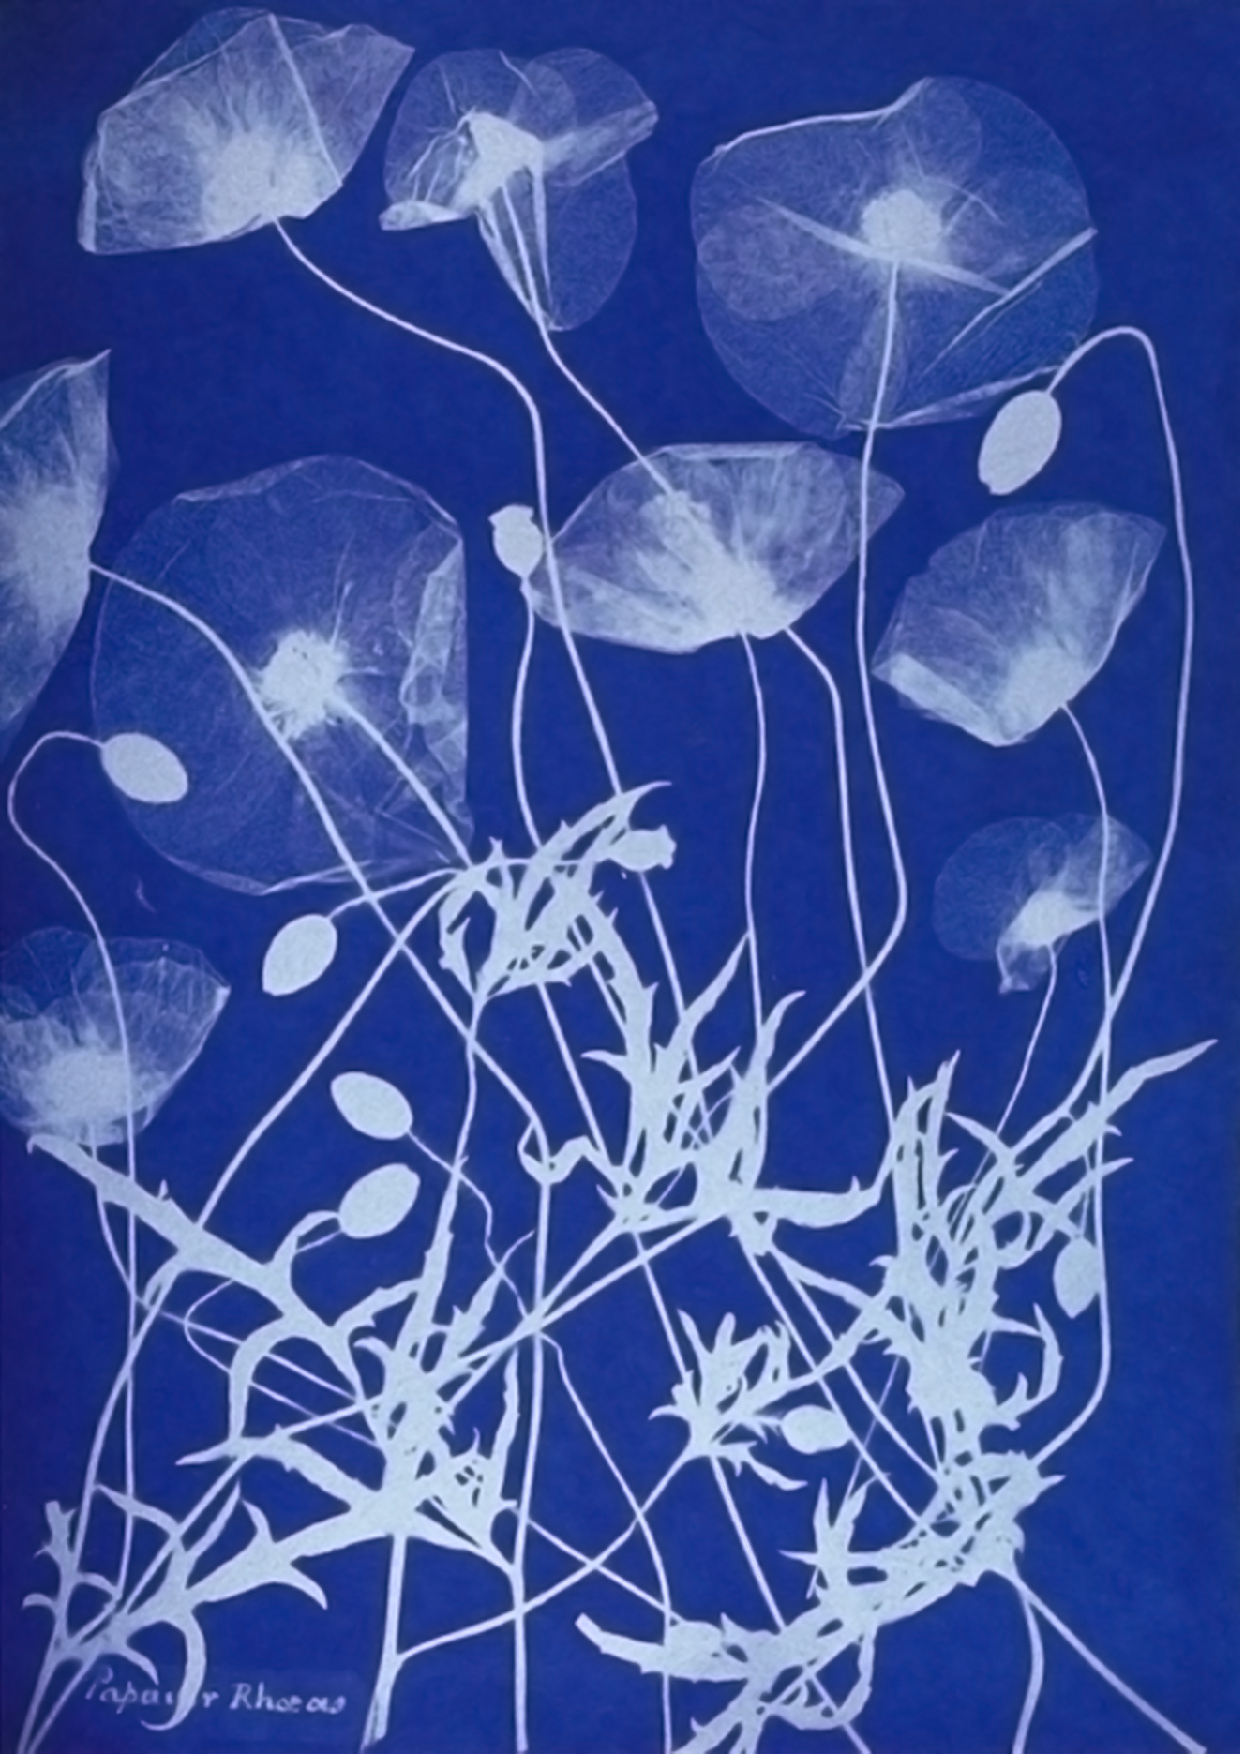
\includepdf{../media/chapter_illustration/papaver_rhoeas}
\chapter{The development of Poppy} % (fold)
\label{cha:poppy-dev}

\section{Introduction} % (fold)

\begin{figure}[tb]
\centering
    \subfloat[][Nao]{\label{fig:nao_platform}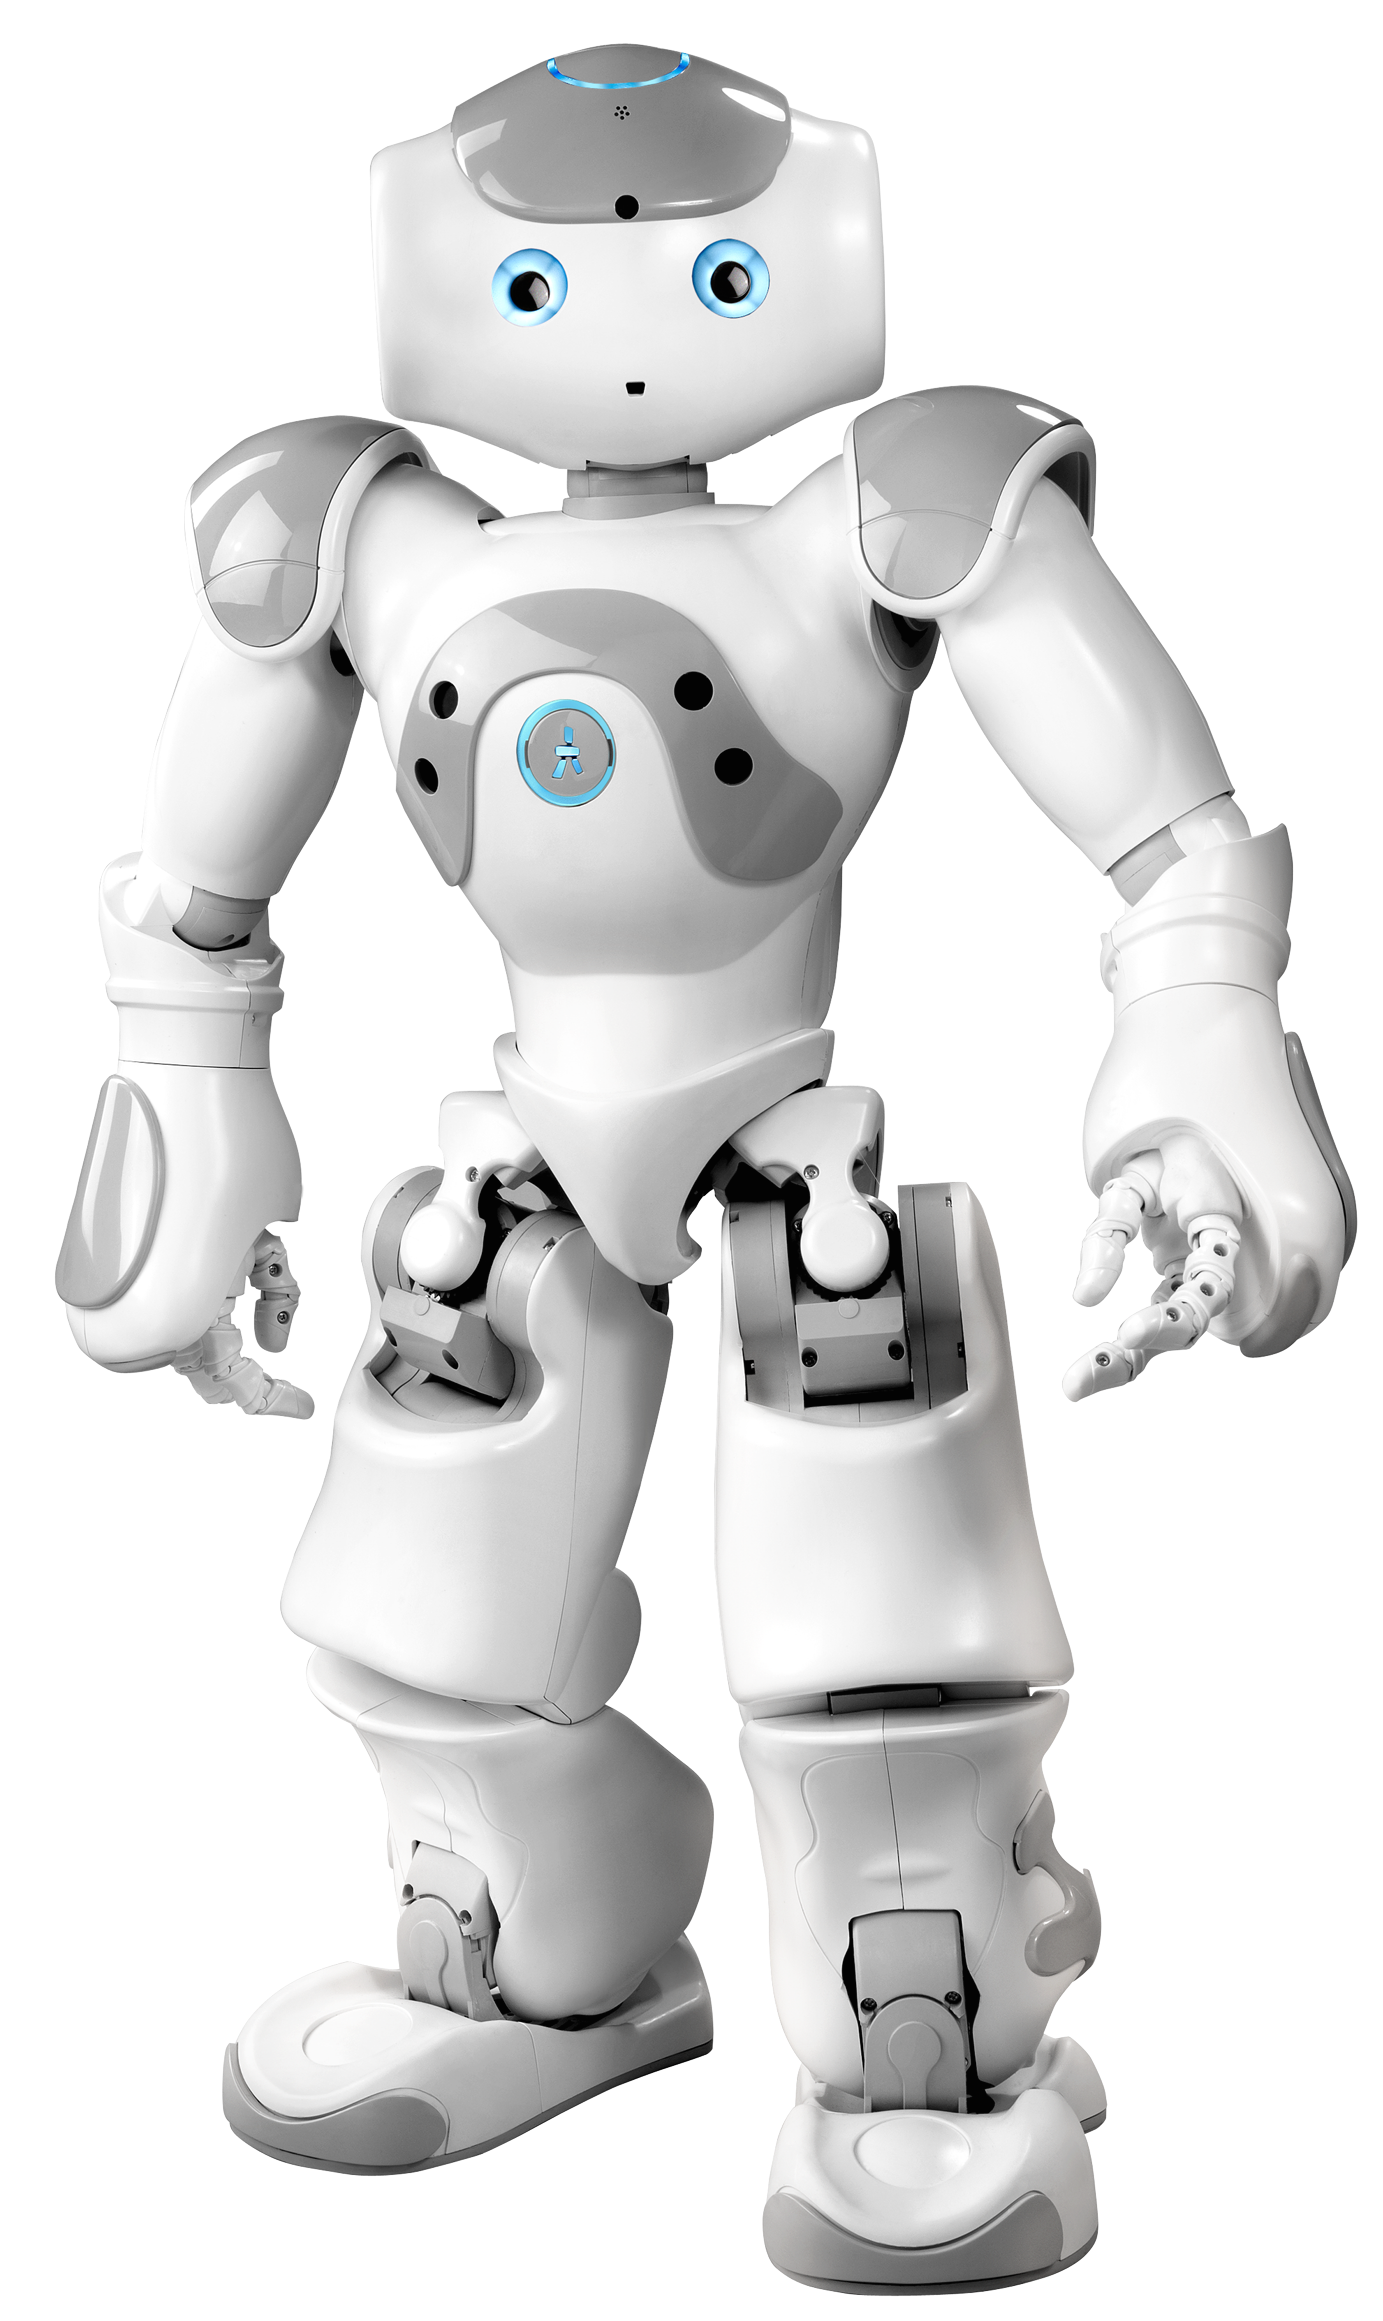
\includegraphics[height=5cm]{nao_face.png}}
    \hfil
    \subfloat[][Darwin-Op]{\label{fig:darwin_platform}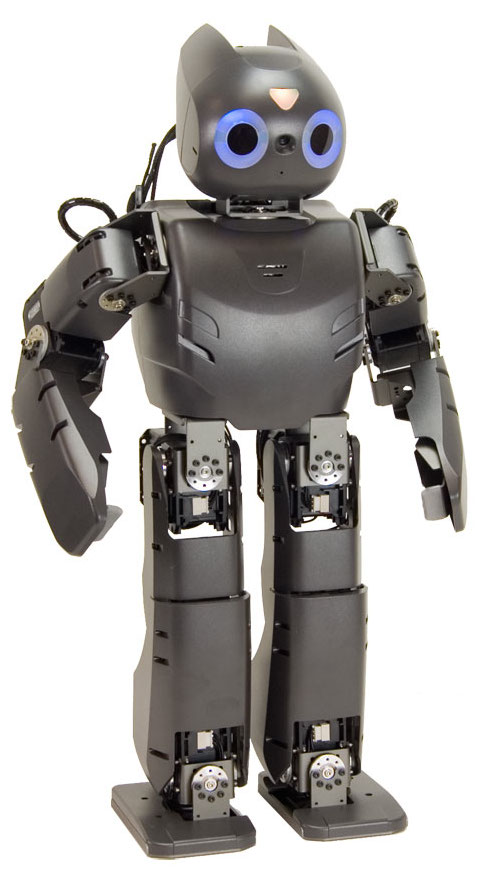
\includegraphics[height=5cm]{darwin_op_face.jpg}}
    \hfil
    \subfloat[][Acroban]{\label{fig:acroban_platform}\includegraphics[height=5cm]{acroban_wout_background.jpg}}
    \caption{None of the existing platforms in 2012 were suitable for exploring the role of morphology. Nao was impossible to modify. Darwin Op and Acroban used aluminium parts that are really difficult and expensive to produce.}
    \label{fig:2012_Humanoids}
\end{figure}

In 2012, when we started this project, none of the existing humanoid platforms were suitable for exploring the role of morphology. There were two kinds of platform. On one hand commercial robots that are rather easy to use and accessible but with a static and frozen morphology. On the other hand, prototype robots produced in labs to address specific experimentation needs, studying interesting morphologies but complicated to use and impossible to reproduce outside the lab. In both cases, only a few are open source, limiting hacks, extensions or modifications of their morphologies even further.

In the Flowers Lab, we had both kinds of robot. We used Nao (see \figurename~\ref{fig:nao_platform}) to study human robot interaction (\cite{rouanet2009integrated} \cite{rouanet2012apprendre}). It was really convenient for use by researchers who are not interested in hardware issue since they are addressing more high-level research challenges. Yet such a platform is limited as it is not possible to modify the robot if it is not strictly adapted to our experiment. For example, back at this time the Nao camera was not efficient, with a closed field of view and a slow framerate. We have difficultly achieved 5 frames/seconds. Although we had the necessary skills to hack Nao and change the camera to fit our needs, its hardware was not designed to be changed. Improving the vision performance would only be possible with the addition of an external camera on the Nao head which could ruin the user experience. In addition, it would have been interesting to explore how the camera parameters (FOV, framerate, resolution...) can change the user experience but again, it is not possible with this robot.


We also used Acroban (see \figurename~\ref{fig:acroban_platform}) designed by Olivier Ly~\parencite{ly2011bio}. It is a handcrafted humanoid platform created to explore certain morphological properties, especially compliance, with the aim of achieving dynamic locomotion and playful physical human robot interaction.
While it actually allows modification of its is morphology, it is manufactured from aluminium mechanical parts, Robotis Dynamixel motors, scotch, and rubber bands cobbled together, and changing it requires lot of effort . The manufacture of aluminium parts required is especially complicated and requires either very good handiwork or a 3-axis CNC.
In addition, its use was quite complicated and while several researchers could have been interested by Acroban to study human robot interaction and social acceptance, It was not possible to use it without significant mechanical work.
Finally, the material and manufacturing process make the platform non-stationary. Even if a lab manages to reproduce it, there is a high probability that the physical properties will not be the same. Therefore, the diffusion and the reproducibility of results are limited.


A last alternative would be the use of Darwin Op robot (see \figurename~\ref{fig:darwin_platform}) which is both open source and easily accessible (Robotis sells it already assembled for \$10K), yet as Acroban its hardware consists of manufactured metal parts making its morphology very difficult and expensive to modify. Moreover, even if Darwin is open source and very popular, to our knowledge its morphology has never be modified by the research community\footnote{We can also notice the lack of community management tools such as wiki, forum and correct versionning system. If someone create a variation of Darwin, there is no place where he can share it.}.

Thus one of the main goals was to successfully design a humanoid robot which can merge the advantages of both kind of robot, i.e. simple, accessible, reproducible and allowing to easily change and hack its morphology for scientific experiments that can be both customized and shared.

\subsection{An experiment-proof robot} % (fold)
\label{sec:experiment-proof}

Most researchers can attest to the difficulty and frustration faced while conducting robotic experimentation in the real world. We are challenged daily by bugs, technical issues, unpredicted events and side effects. While a bug in software can be fixed, an error with a hardware platform can cause damage to the robot and postpone the results of an experiment by several weeks.

Therefore many researchers in robotics avoid technical issues associated with the real world experimentation by using simple models and physical simulation. But the real world is extremely more complex and richer than the virtual one.
Some high-level behaviour experiments are conducted in simulators based on the hypothesis that real-world constraints are not relevant, yet it is really certain?
Indeed, while the real world constitutes a lot of constraints, it is also rich in complex physical effects (gravity, friction, inertia), which should be taken into consideration and could be very useful if interacting with the agent.

As we saw in the related work (chapter~\ref{cha:morphology-review}), the emergence of complex behaviours appears thanks to the interaction between the real world and simple robotic systems. We cannot program behaviour because behaviour is the result of interaction  between the program and the real world. Thus we cannot design behaviour without the ecological niche of the robot~\cite{Steels1991emergence}.

While using simulators can be helpful as a first step to design robots, it appears incomplete when showing results on the role of morphology without real world experimentation.
Therefore, when one wants to study the role of morphology on robot behavior, being able to explore it in the real world is of paramount importance. Unfortunately, current tools make the experimental step really hard to achieve for researchers.

Throughout our work on building cognitive and developmental learning algorithms, we have experienced these issues, especially while building and using Acroban~\cite{ly2011bio} and during the Ergo robot experience (see chapter~\ref{cha:art}). Much time has been spent debugging non-robust technologies but it has been very instructive for understanding those that are efficient and those that should be avoided.
Therefore Poppy has been designed based on the background experience we have acquired building using robots acting in the real world.

\begin{description}
    \item[Robustness and Safety:] Demanding and lengthy real-world experimentation necessitates that the robot be robust and safe. It should be able to sustain experiments and fall down without easily breaking. At the same time, one should ensure that physical interaction with the robot is safe for humans.
    \item [Precision, stationary:]Experiments should be repeatable, implying that the robot properties should be stationary.
    \item [Breakable, repairable:] Breaking should not be costly and the robot should be easily repairable.
    \item [Transportable:] To allow for experiments in natural environments, possibly involving interaction with non-technical humans, the robot should be transportable outside the laboratory.
    \item [Easy and fast to duplicate:]If the robotic platform is to be reused  in this way, it must be easy and fast to duplicate.
    \item [Affordable:] To ensure widespread use, a key factor is to keep the cost of the platform relatively low. The more labs can be involved, the greater the scientific impact.
\end{description}

To respond to these needs we created Poppy (see \figurename~\ref{fig:poppyv0.1_overview}).

\subsection{Overview} % (fold)

Poppy is a small and lightweight 25-DoFs humanoid robot (see section~\ref{sec:poppy-modularity}), whose morphological design allows for quick and simple modification by non-expert people. This is achieved thanks to the use of the 3D printing technique for the mechanical structure and Arduino based electronics architecture (see section~\ref{sec:poppy-electronic}). Its motors are common and widely used off-the-shelf Robotis actuators, and allow for compliant control and soft physical human-robot interaction. The pypot library (see chapter~\ref{cha:pypot}) enables programming beginners as well as advanced roboticists to control the robot and is adapted to the modularity of Poppy’s hardware.

\begin{figure}[tb]
    \begin{center}
        \includegraphics[width=0.95\linewidth]{poppy-overview.pdf}
    \end{center}
    \caption{Overview of Poppy beta with the main specs and features. This figure will be updated when the final release of Poppy is ready.}
    \label{fig:poppyv0.1_overview}
\end{figure}

Its current morphology takes inspiration from the human functional morphology: a large number of joints (25 motors), the limbs respect human proportions, it has five joints in the torso and its thighs are bended by a $6\deg$ angle, similar to human ones (see section~\ref{sub:poppy-leg-design}).

All the work and material involved in building, creating and using Poppy is distributed under open source and open hardware licenses. The 3D-printed skeleton and the electronics boards are under Creative Commons licenses while the pypot library is distributed under GPLv3 licenses.

Poppy is the first open source and 3D-printed complete humanoid robot, the design of such a novel platform will be discussed in the following sections.


\section{Exploring morphological variants} % (fold)
\label{sec:poppy-modularity}

The whole structure must be easily reconfigurable both for the purposes of repairing and hacking. This means the process of replacing Poppy's parts must be simple, low-cost and not require time or special tooling. Also, in order to have a real impact in the open hardware community, special attention is given to the modularity and the reusability of our technological bricks.
Poppy is fully modular (mechanic, electronic, software) allowing freely exploration and modification of Poppy's body.
Its modularity and the use of 3D printing make Poppy highly hackable. Therefore it can be easily adapted to particular experimental setups and allows diverse exploration into its morphology.


\subsection{3D printed parts} % (fold)

We introduced for the first time the use of 3D-printed mechanical parts in our work when we built the ergo-robot installation (August 2011 - see chapter~\ref{cha:art}). The result was impressive as the parts were robust, precise, low-cost and fast to produce. Very convinced by this technology and with a keen desire to be free to explore robot morphology, we decided to build the whole mechanical structure of Poppy based on 3D printing techniques.

\subsubsection{Technique used} % (fold)

Several 3D techniques exist and were presented in the related work (see chapter~\ref{cha:3Dprint-OSH}). The Stereo-Lithography\footnote{This technique relies on a photosensitive monomer resin, which forms a polymer and solidifies when exposed to ultraviolet (UV) light.} (SLA) is very precise yet the material is not well adapted to support mechanical stresses.

Alternatively, we can use Fused Deposition Modelling\footnote{The FDM technique relies on melting and selectively depositing a thin filament of thermoplastic polymer (ABS - PLA) in a cross-hatching fashion to form each layer of the part.} (FDM), which has the great advantage of being very low cost (2000\$ for the printer + 40\$/kg of material) and therefore, accessible directly in the lab. The parts produced are good yet the finish is not perfect and often needs to be reworked by hand. Also the process creates non-uniform parts, less resistant on one axis. Above all the FDM printers have low reliability, leading to a large number of printing failures. Nevertheless low-cost FDM printers are really useful when we just want to produce initial or single-use parts.

We prefered the use of Selective Laser Sintering (SLS)\footnote{The process uses a high power (25-50W) CO2 laser beam, which melts and fuses fine powdered material spread on a layer.}. This 3D printing process allows the production of almost any shape without constraint. In addition, the price of the part depends on the total size and not on the complexity of the shape. This permits the production of very optimized shapes without increasing the total price of the robot. Moreover the use of polyamide material produces high quality parts with very good mechanical properties: uniform, lightweight, flexible and robust.

The table~\ref{tab:materials} compares mechanical properties of polyamide with classic metallic materials. We can see the relatively good properties of the polyamide material. The young modulus represents the stiffness of the part. The polyamide one has a very low young modulus meaning it is very flexible while keeping correct yield strength and very low density.

\begin{table}[tb]
    \centering
    \begin{tabularx}{0.8\linewidth }{l X X X}
        \textbf{Material} & \textbf{Mass Density $\rho$ ($kg/m^3$)} &  \textbf{Yield strength $\sigma$~($MPa$)} & \textbf{Young Modulus $E$($GPa$)}\\
        % \hline
        Polyamide & $930$ & $49$ & $1.65$\\

        Aluminum & $2700$ & $200$ & $70$\\

        Steel & $7500-8000$ & $350$ & $200$\\

        Titanium & $4500$ & $1200$ & $114$\\

    \end{tabularx}

    \caption{Comparison of material properties.
    The Young modulus represents the stiffness of the material while the yield strength corresponds to the maximal stress tolerable before plastic deformation.}
    \label{tab:materials}
\end{table}

A SLS printer is much too costly for a lab, but outsourcing the production to an external company\footnote{\url{http://i.materialise.com/}} is really easy\footnote{In most cases, the company offers automatic scalable orders through an on-line platform} and relatively low cost\footnote{Printing all the parts to build a Poppy costs about 1200\texteuro HT.}

\subsection{Exploring morphological variants} % (fold)


3D printing is a key feature of Poppy that permits the exploration of morphological variants. Indeed it is now cheap and easy to produce custom parts, and because Poppy is open source, anyone has access to the source files and can freely change the parameters he or she wants. Indeed Poppy is designed using Solidworks, a parametric CAD Software very widespread in small-size engineering companies. The parametric modeling allows to create mechanical parts those design are based on a set of parametric sketches and functions. Parameters can be modified and the final part will be changed accordingly\footnote{If designed correctly}. Therefore it is possible to easily change the mechanical structure and properties just by tuning associated parameters in the source file and re-printing the part (see \figurename~\ref{fig:exploring-morpho-poppy}).

\begin{figure}[p]
    \centering
        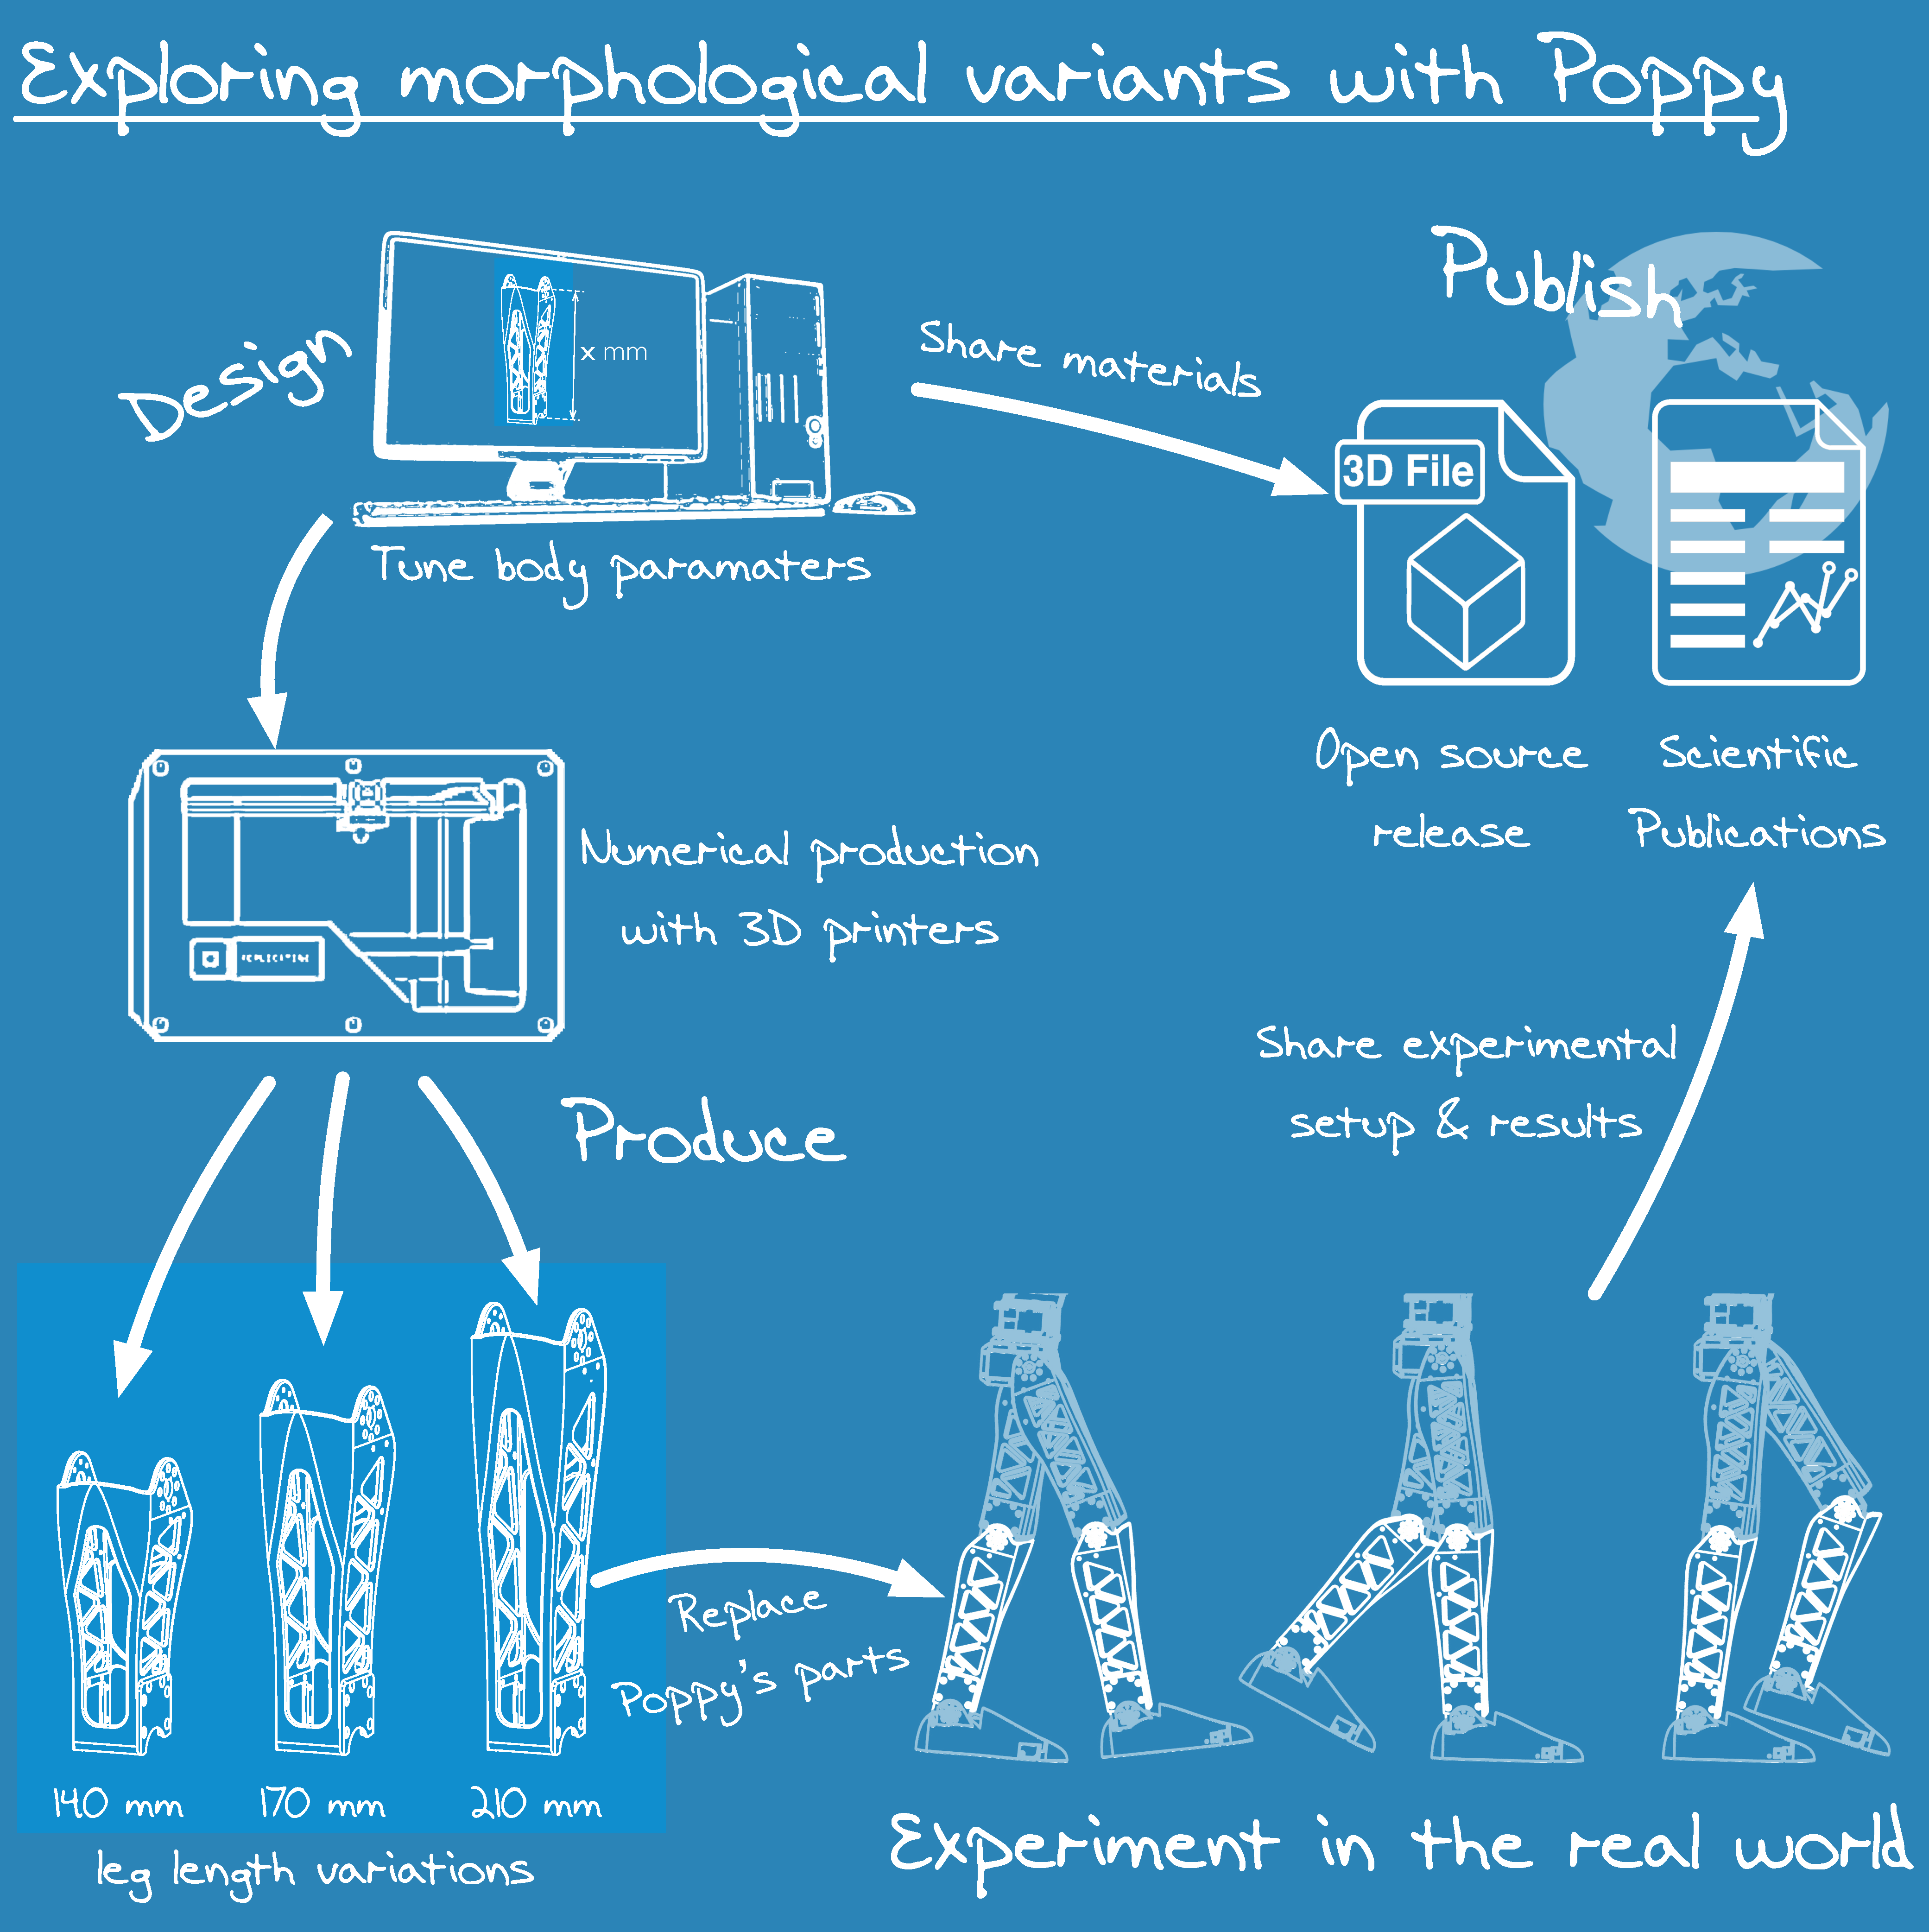
\includegraphics[width=\linewidth]{morpho_variation.pdf}
    \caption{The use of 3D printing open new perspectives to explore the role of morphology in the robotics field. Indeed we can now easily produce on site new mechanical parts, therefore it is possible to create numerous variations of body properties. Poppy's modularity makes the part substitution easy and fast so we can directly iterate with real world experiments. Then we can share online a reproducible experimental setup.}
    \label{fig:exploring-morpho-poppy}
\end{figure}


Moreover, 3D printing does not only permit the shape of a part to be changed, it can actually produce it with different materials. In particular, Direct Metal Laser Sintering (DMLS) - very similar to the SLS process - permits to produce the same parts using materials such as steel\footnote{http://i.materialise.com/materials/stainless-steel} or titanium\footnote{\url{http://i.materialise.com/materials/titanium}}. It is therefore possible to extend the exploration to material mechanical properties (e.g. flexibility, density).


\subsection{Scalable actuation} % (fold)
\label{sub:scalable-actuation}
As explained in chapter~\ref{cha:methodology}, the chosen methodology relies on the all-in-one Robotis actuator. They are really convenient to use as they directly embed drivers, encoders and communication buses. They are also quite powerful, robust and rather precise. This is done by the combination of Maxxon motors, metal gearbox and precise magnetic rotation sensor (resolution: 0.1\textsuperscript{o}).

Also Robotis offers a range of motors with different actuation power (see \figurename~\ref{fig:dynamixel_powa}). They are different in size and power but their API remains the same and we can easily switch from one to another without either changing the code or the electronic integration. Yet, even if the size changes, the footprint keeps the same pattern (see \figurename~\ref{fig:dynamixel_dimension}).

Poppy is designed with Solidworks, a parametric modeler that offers features like configurations which define sets of parameters. Configurations allow to create multiple variations of a part or assembly model within a single document. Configurations provide a convenient way to develop and manage families of models with different dimensions, components, or other parameters. It is therefore possible to create, for each part, a configuration compatible with each motor just by setting the suitable parameters. The \figurename~\ref{fig:leg_configuration} shows an example with Poppy's leg.


\begin{figure}[p]
    \centering
        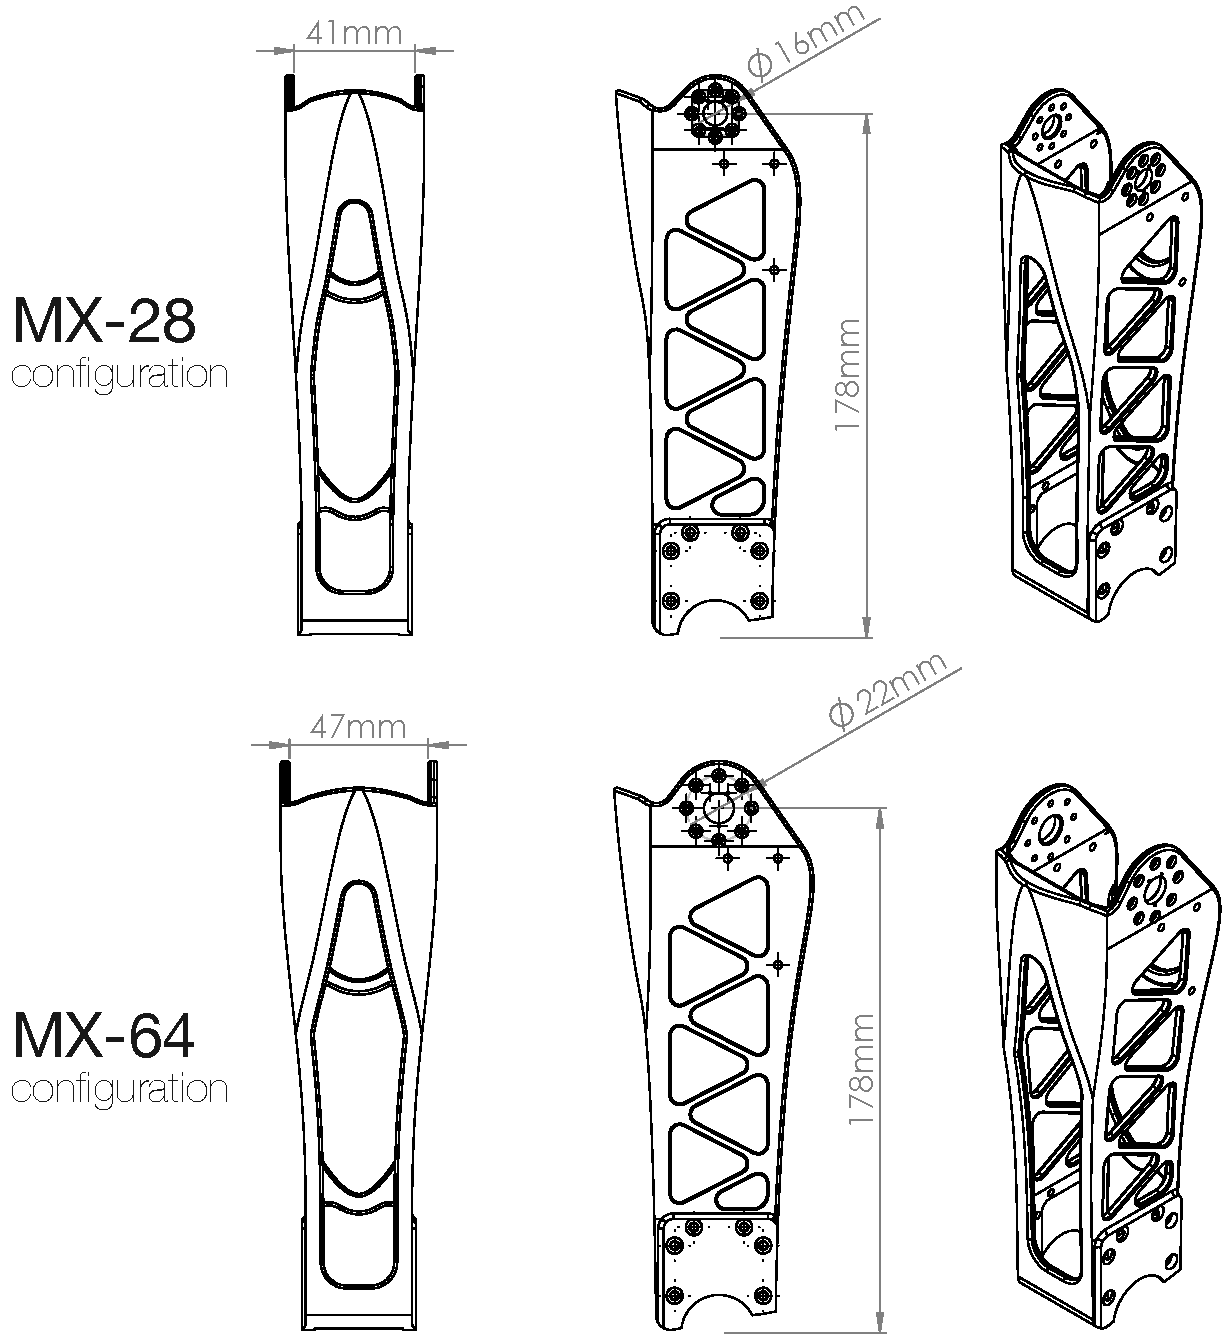
\includegraphics[width=\linewidth]{leg_configuration.pdf}
    \caption{Example of the use of mechanical configuration. Here the CAD source of the leg involves 2 configurations so it can be compatible with Dynamixel MX-28 (up) or Dynamixel MX-64 (down). Configuration define the set of parameter suitable for both and can be changed just in one mousse click.}
    \label{fig:leg_configuration}
\end{figure}

It just takes a couple of minute to transform a part designed for Dynamixel MX-28 to one compatible with Dynamixel MX-64 as we only have to change the parametric dimensions accordingly to the Robotis motor shape. Then it is possible to switch from one to another with one click.
On Poppy, most of the parts are already distributed with multiple configurations suitable for different motors power. It allows the actuation power to be scaled and introduces it also as an experimental (discrete) variable.


\subsection{Electronic} % (fold)

Unlike the mechanical parts, there is no quick and low-cost solution for producing custom electronics yet.
However, exploring morphology may also require the sensors space (e.g. number, type, properties, positions) to be varied. As we explained in the chapter~\ref{cha:morphology-review}, we address this challenge through the use of the Arduino environment.

Arduino has developed both hardware and software, so creating and programming electronics systems becomes very easy. Their boards have plenty of I/O pins (digital and analog) suitable to power and control almost any electronics components. Also these pins can be used to handle low-level communication such as UART, SPI and I2C, useful to plug sub-module (e.g. IMU, LCD Matrix, tactile interface and so on).
The software they developed abstracts the complexity of low level control\footnote{we can turn a led on/off with just one line of code.} and communication\footnote{Using just print-like functions we can communicate on serial bus.} very well. Therefore, it allows wide variety and flexibility in the extension of the electronic system, while keeping an ease of use adapted to a non-expert audience.
In addition, Arduino has a growing community - already relatively large - which creates, shares and produces low-cost, various and multipurpose electronic components. Actually almost all kinds of sensors have an Arduino version with ready-to-use hardware and software.

Being able to change the morphology easily is of paramount importance in the Poppy project. Using Arduino-compatible architecture permits electronic modularity, which means the sensory-motor space can be considered as an experimental variable.


\section{Lightweight} % (fold)
\label{sec:lightweight-robot}

Many humanoid robots use powerful motors often associated with highly accurate sensors. This has a cost, both in terms of weight and computation resources. Moreover, to ensure the accuracy of the sensory-motor space it is necessary to design very rigid mechanical parts. The whole structure obtained is powerful but very heavy and not very agile due to inertia.
In the Poppy platform, lightness is very important both for dynamic properties and safety:
\begin{itemize}
    \item for a given actuation power, reducing the link mass reduces its inertia and permits the agility and the responsiveness to be increased,
    \item makes Poppy a platform that is easier to manipulate and transport outside the lab,
    \item makes the robot safer for people as well as for itself when it falls (and it will definitely fall a number of times).
\end{itemize}

\begin{figure}[!t]
    \centering
        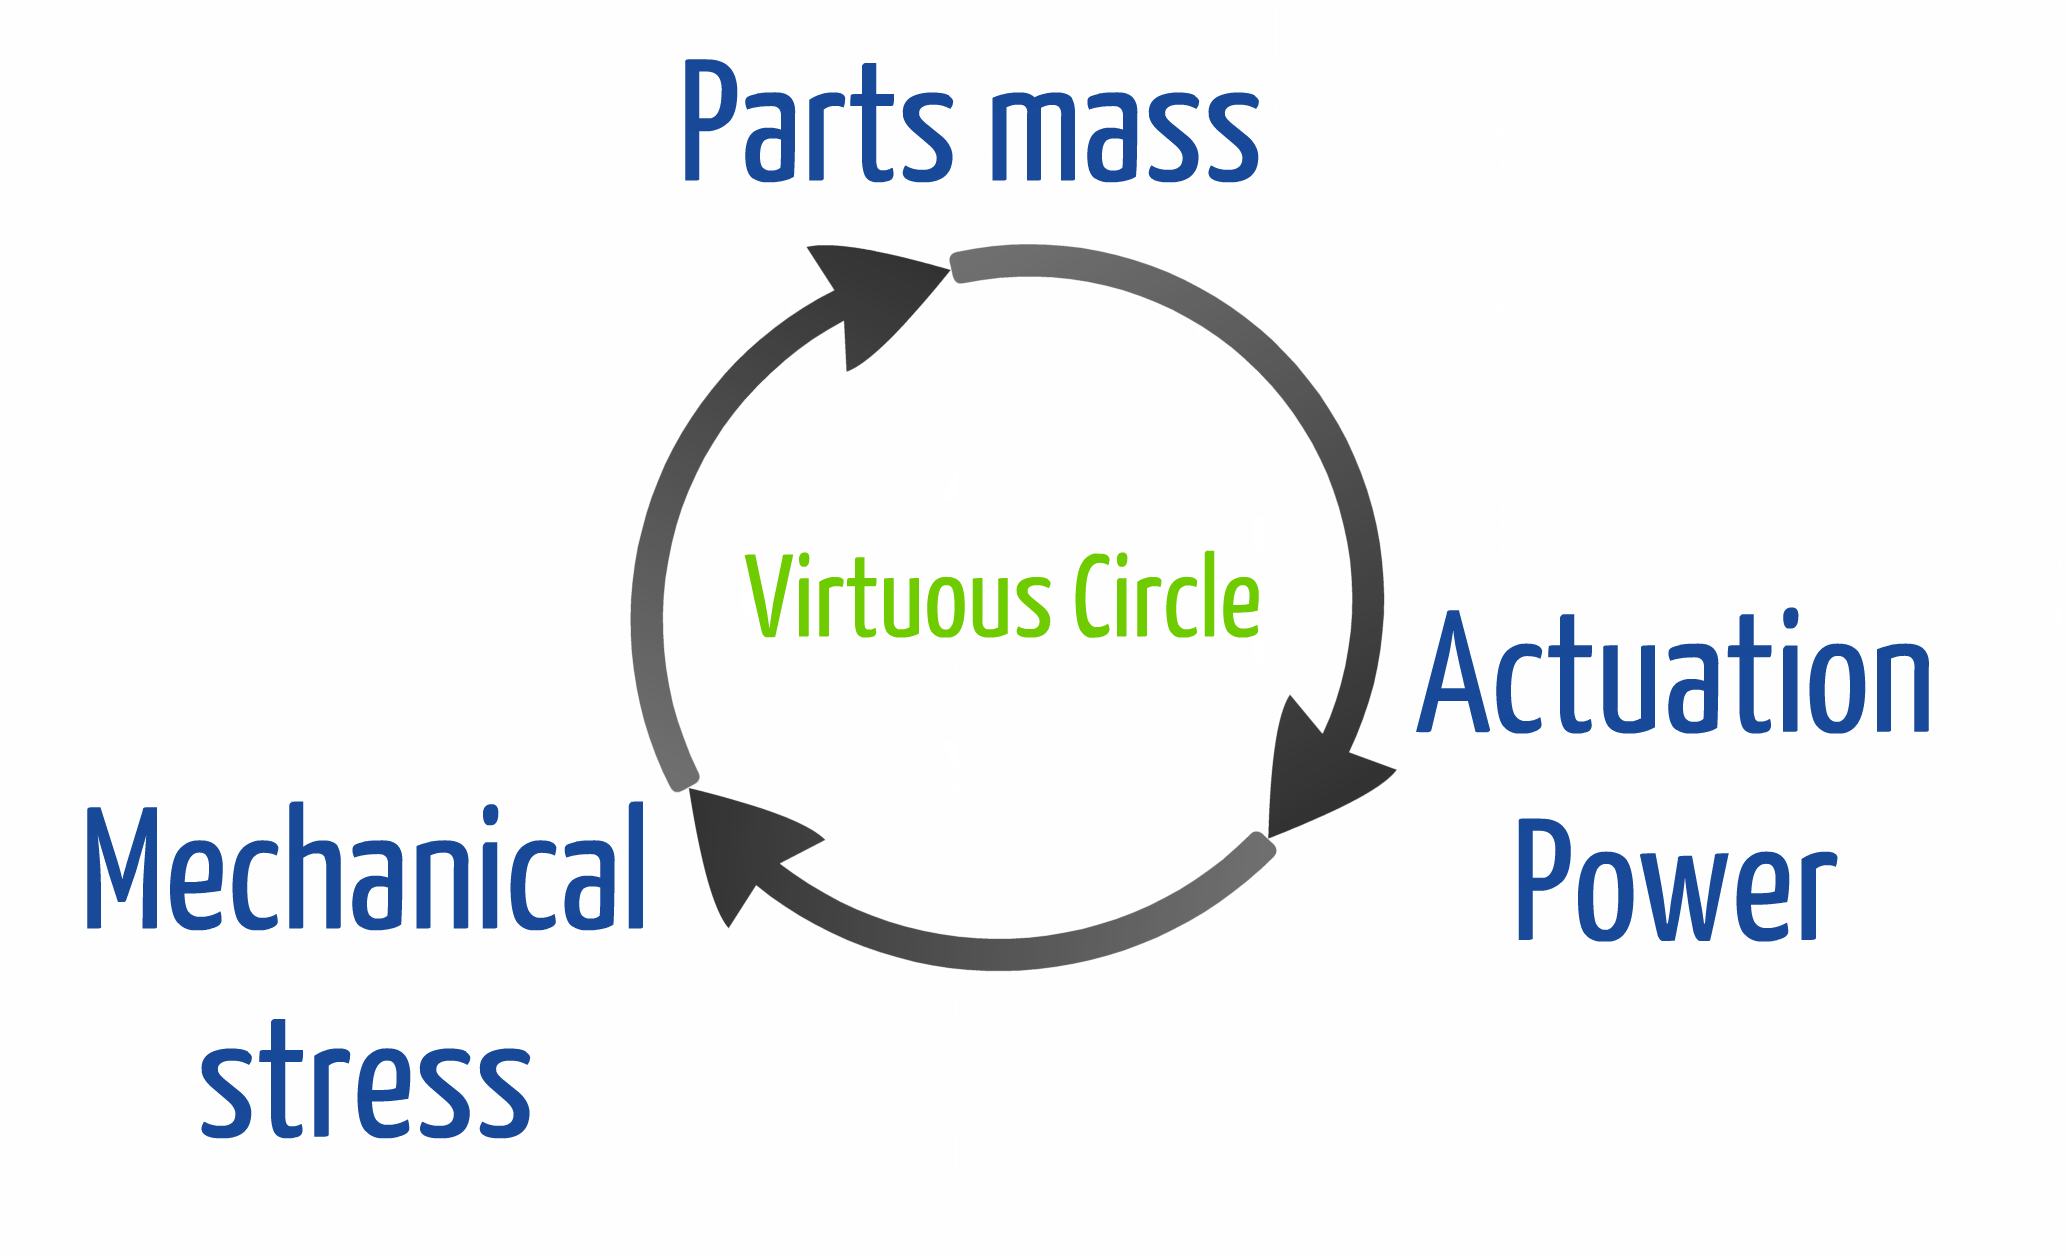
\includegraphics[width=0.6\linewidth]{virtuous_circle.png}
    \caption{Using small actuation power reduces the amount of stress applied on the mechanical structure. Thus it is possible to reduce the robustness of mechanical parts by removing matter. Because the global weight is reduced, we can use smaller actuation power, and so on.}
    \label{fig:virtuous_circle}
\end{figure}

The lightness was achieved by combining low-power actuation and optimized structure. Indeed when combined, it creates a kind of virtuous circle where the reduction of the maximum torque reduces the strength on mechanical parts. Because less force intensity is applied, we can remove material from parts. Because we have a lighter mechanical structure we can reduce the actuation power required and so on.


Also using low-power actuation has several interesting advantages:

\begin{itemize}
    \item The actuation being the main cost of the robot (>60\%), using the least powerful motors significantly reduces the total cost of the robot.
    \item Low-power actuators mean a safer robot. Indeed, in the case of a programming error, the robot is not powerful enough to hurt someone or itself.
    \item on a research challenge level, it constrains the possible movements to the ones requiring little strength, the result being certainly more human-like.
\end{itemize}

Therefore Poppy was designed using the weakest and lightest motors i.e. MX-28\footnote{Robotis motors are quite heavy (72, 126 and 153g respectively for MX-28, MX-64 and MX-106) in comparison of the Futaba servo-motors, 20-50g for a comparable output torque see \url{http://www.futaba-rc.com/servos/brushless.html}}, except for a few particular joints (such as the hips) while the mass reduction of the mechanical parts was achieved by using truss design.

Truss is a well-known design technique from structural mechanics to create lightweight yet very robust structures. It is mainly used in civil engineering (see \figurename~\ref{fig:truss_bridges}) but can also be used in planes, which require lightness and strength resistance.

\begin{figure}[tb]
    \begin{center}
        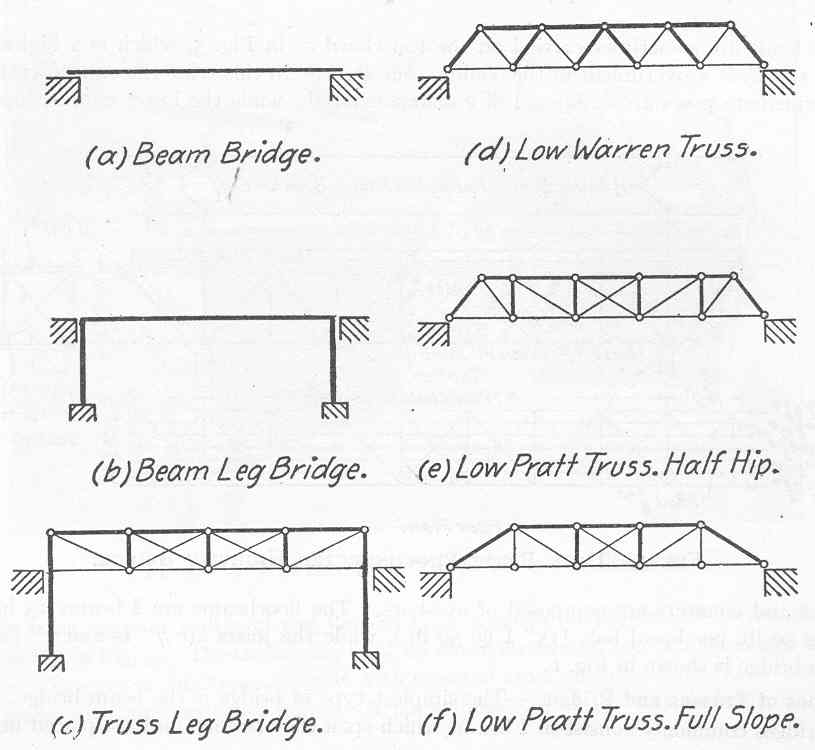
\includegraphics[width=0.5\linewidth]{truss_bridges.jpg}
    \end{center}
    \caption{The truss structure has been massively used in civil engineering, especially to construct bridges. Here is shown several truss structure configurations.}
    \label{fig:truss_bridges}
\end{figure}


The principle is based on beam theory and permits to increase the second moment of area of a beam cross-section (see \figurename~\ref{fig:leg_section}), which is an important property in the calculation of deflection, the main weakness of a long beam.

The second moment of area is computed as follow:
\begin{center}
    $I_x = \iint_s y^2 dxdy$

    $I_y = \iint_s x^2 dxdy$
\end{center}
where $s = dxdy$ is the surface integrated along the two axes of the cross-sectioned surface. We can see the  on each dimension varies with a quadratic factor meaning the variation is not linear. Therefore matter placed far away from the origin is much more effective in increasing the second moment of area.
Thus the main idea is to remove -the no effective- matter at the center and place it on the rim. In truss structure, matter is assembled by linkage avoiding local deformation.

\begin{figure}[!ht]
\centering
    \subfloat{\label{fig:Poppy_leg_section}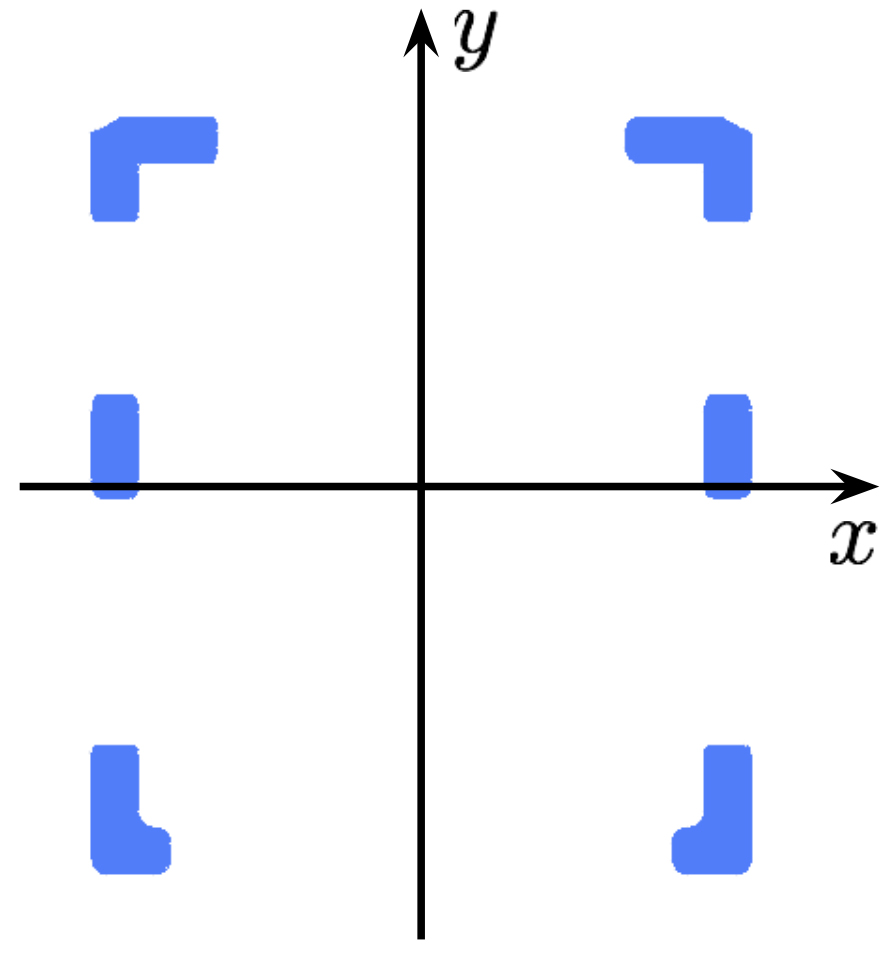
\includegraphics[height=2.5cm]{Poppy_leg_section.jpg}}
    \hfil
    \subfloat{\label{fig:basic_leg_section}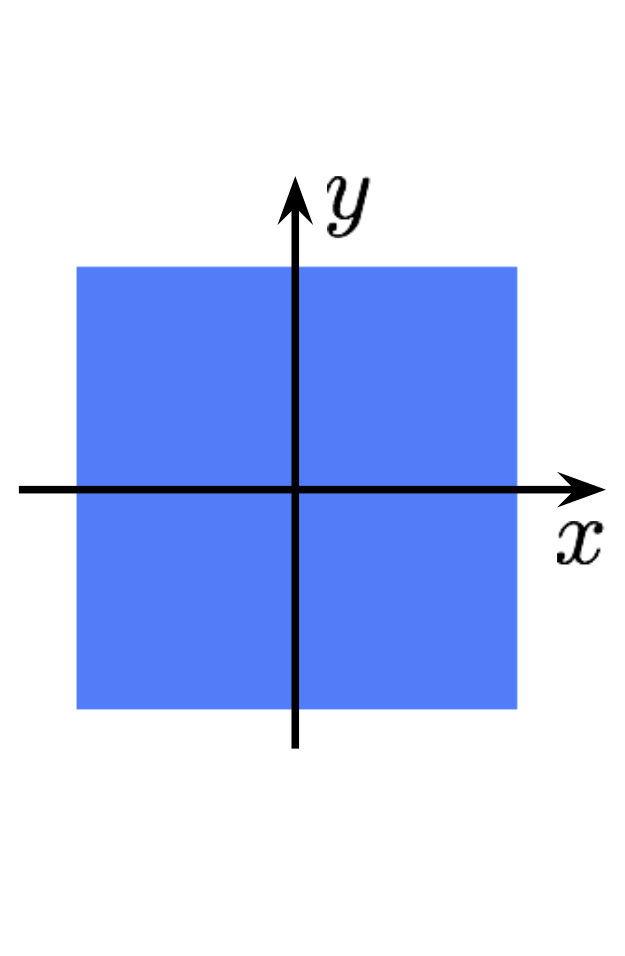
\includegraphics[height=2.5cm]{basic_leg_section.jpg}}
    \caption{Comparison of poppy's leg section and a rectangular beam having the same second moment of area.}
    \label{fig:leg_section}
\end{figure}

The \figurename~\ref{fig:leg_section} shows the comparative cross section of two beams with the same second moment of area value. More precisely, the \figurename~\ref{fig:Poppy_leg_section} is a cross section of Poppy's leg while the figure \figurename~\ref{fig:basic_leg_section} is a basic beam with a rectangular profile.
It would require a section such as $b=27.72 mm$ and $h=27.59 mm$ for the rectangular to have the same quadratic momentum as the truss design (i.e. $I_x = 54.862 mm^4$ and $I_y = 53.260 mm^4$ measured with Solidworks).
Considering the length of the leg part (i.e. $190 mm$), the total mass would be equal to $142 g$ instead of $47 g$ for the actual leg. This corresponds to a reduction of 70\% of the mass.

\begin{figure}[!tb]
\centering
    \subfloat[][Poppy's arm mechanical structure]{\label{fig:poppy_arm_truss}\includegraphics[width=0.49\linewidth]{arm_truss.jpg}}
    \hfill
    \subfloat[][Poppy's leg mechanicalt structure]{\label{fig:poppy_leg_truss}\includegraphics[width=0.49\linewidth]{leg_truss.jpg}}
    \caption{The whole design of Poppy is based on the use of truss structure to reduce its weight while keeping sufficient robustness.}
    \label{fig:poppy_truss_structure}
\end{figure}

All of Poppy’s limbs are based on this structure and have been optimized using finite element analysis (FEA) to perform structural simulation and validate the performance and safety factors of parts.
Thanks to the use of this design on all of Poppy's limbs (see \figurename~\ref{fig:poppy_truss_structure}), we managed to have -certainly- the most lightweight humanoid robot with 3.5kg relative to its 83 cm height.

\clearpage
% !TEX root = ../../thesis.tex
\tikz[remember picture,overlay] \node[inner sep=0pt] at (current page.center){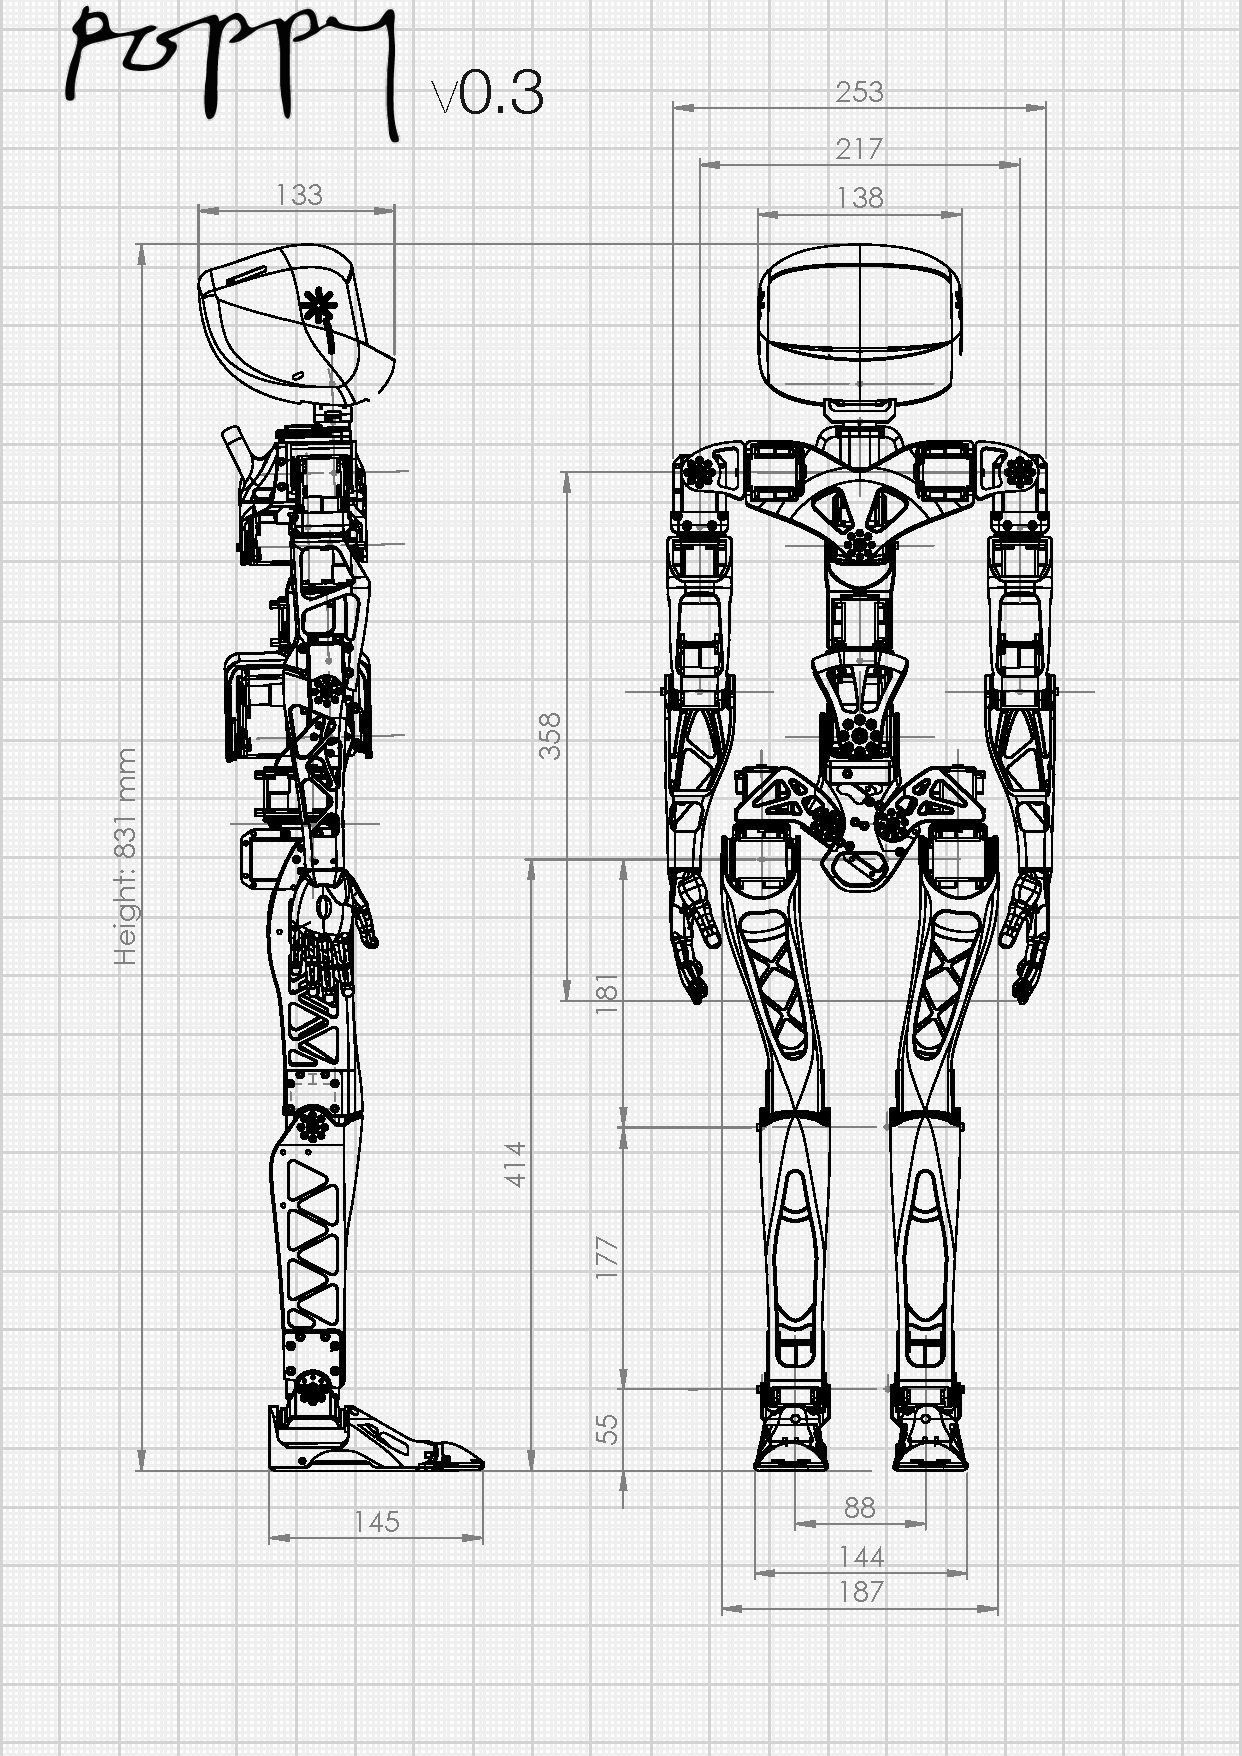
\includegraphics[width=\paperwidth,height=\paperheight]{Poppy_dimensions}};
\clearpage

\section{A little robot} % (fold)

To reach the goals presented in the introduction, the size of the robot is a really important aspect.

On one hand, small size makes the integration of complex, powerful and accurate mechatronics very difficult. Therefore it reduces the scope of technology we could use for the robot. In particular, the integration of hydraulic and pneumatic actuators, as well as advanced mechanisms involving several moving parts is really challenging.

On the other hand, having a small robot is really convenient for exploring morphological properties in the real world.

Firstly, it changes significantly the experimental process: the ratio between weight, and thus energy and torques enforced by movements, and the mechanical robustness of the structure and of the actuators, is such that the robot can fall without breaking itself. Moreover, it is lightweight, which allows people to handle it directly without additional infrastructure and in a safe way. On the one hand, all of this speeds up the experimental process. On the other hand, it deeply changes the methodology of movement and motor skill design by allowing the creation of movements directly on the robot by real-world experiments without a simulation process. This includes for instance adjusting motor primitives in real time, even critical ones.

Secondly, this brings advantages regarding human interaction, which is an important focus in this work: on one hand, from the above reasons, this rules out the problem of physical security in Human/Robot interaction. On the other hand, the size of the robot plays an important role in the psychological representation that people have of it.

However exploring morphological properties requires having a robot those morphology has an actual impact on its dynamic. Being too small reduces this impact because it reduces the inertia and the role of intrinsic structural frequency.

Thus Poppy's size is a compromise to facilitate at the same time easy testing in the real world, the integration of a large number of degrees of freedom (25 DoFs) and a structure those dynamic properties cannot be neglected.

\subsection{Morphological proportions} % (fold)

From an anatomical point of view, Poppy reproduces the human proportions as described in the literature~\parencite{dufour2005biomecanique} (see Fig. 3) and the sensorimotor space organization: i.e. the main degrees of freedom (actuated and passive).

As the human grows from child to adult, his body proportions change~\parencite{bogin2010leg}. One hypothesis we made is that human proportions converge toward an optimal link ratio. Based on this hypothesis we decided to respect the human body proportion of an adult, thus the size of the robot described previously (see section REF) has defined all\footnote{An exception was made for the head, which is bigger to make it cuter and will be discussed in section REF.} dimensions  of Poppy's links with the proportions presented on \figurename~\ref{fig:poppy-human-proportion}.

\begin{figure}[tb]
    \begin{center}
        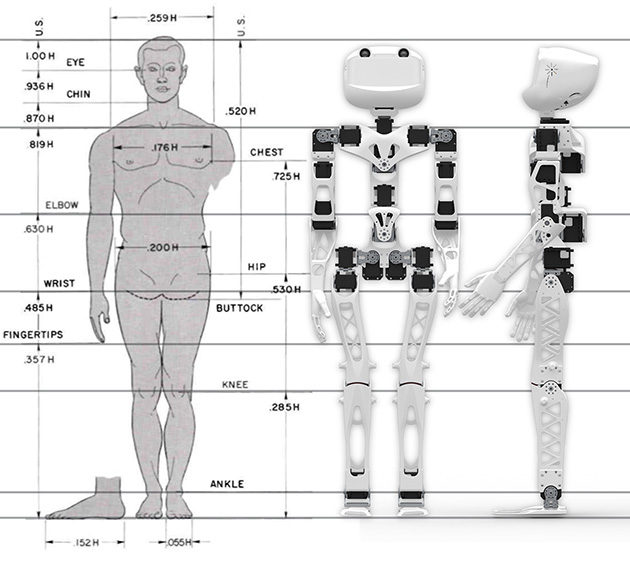
\includegraphics[width=0.8\linewidth]{proportion_poppy.jpg}
    \end{center}
    \caption{}
    \label{fig:poppy-human-proportion}
\end{figure}

Of course, this hypothesis is contestable, and for example, mimicking the proportions of a child  the same size as Poppy could be as relevant. Yet this choice has been taken as a starting point and thanks to the design methodology we have and the open source diffusion, anyone can easily explore other choices and compare them.

\subsection{Small and lightweight feet} % (fold)

With the goal of achieving biped locomotion, most humanoid robots have big, flat and rectangular feet. This design is indeed really convenient to simplify balance problems while easily increasing the sustentation polygon, but this design choice carries some constraints:

Firstly, increasing the foot size increases the lever arm applied to the ankle. It can be useful as it extends the impact of the ankle control over the whole body. Yet given the potential high-torque applied to the ankle, achieving such control requires very powerful actuators.
Powerful actuators are heavier and therefore the whole actuation design of the robot needs to be powerful in order to be able to lift and move the feet.

Secondly, some interesting dynamic controllers for biped locomotion seem to require mass-less legs~\parencite{hyon2002development}. Indeed, in this case there is no moment of inertia due to the motion of the legs, therefore controlling the whole body is simplified. While this case is a theoretical trick, it can still be transferred to the real world if there is a strong trunk/legs mass ratio. Therefore, either the overall mass of the robot should increase in order to make the mass of the legs negligible or we should design more lightweight legs.
Because they are the furthest element from the torso, the mass of the feet has a strong impact on the inertia of the legs.

Finally, while current state of the art robots show that it is still simpler to achieve biped locomotion with big and heavy feet, some projects show impressive results thanks to the use of small or flexible feet~\parencite{bruneau2001dynamic}. We can cite in particular Petman (see figure REF) who demonstrates cutting-edge skills in biped locomotion over very complex terrain\footnote{Link youtube}.
Moreover this aspect seems to be coherent with multi-legged animal species, indeed most animals have really thin legs and very small feet (see fig REF).

So even if common humanoid robots still use big and powerful feet, for the above mentioned reasons, we decided to explore bio-inspired, small, and lightweight feet.

While the human foot is very complex system involving dozens of bones, muscles and tendons, we simplified the design by extracting a few relevant functional human foot properties such as toes, which are key features concerning in both human walking~\cite{Hughes1990} and biped robots with a human-like gait~\cite{Sellaouti2006}. On Poppy's feet, to reduce the weight and complexity, we designed a passive articulation with torsion spring (see figure REF).
Also Poppy has very small feet compared to common humanoids, the ratio of height/length of feet is close to the human one at about 17\% while robots such as Nao have feet that represent 27\% of its height (see table REF).

\begin{table}[ht]
\centering
\begin{tabular}{l| c c c c c}
    & Human & Nao & Darwin Op & Nimbro-OP & Poppy \\
    \hline
    height (cm) & NA & 58 & 45 & 20 & 83\\
    Foot length (cm) & NA & 16 & 23 & 20 & 14.5\\
    ratio (\%) & 16 & 27 & 23 & 20 & 17\\
\end{tabular}
\caption{}
\label{tab:poppy_feet_compare}
\end{table}

Finally, unlike most humanoids, Poppy has only one active DoF. Indeed, while Poppy has small feet, it appears the actual moment it can transmit to the ground is really little for the lateral motion. Also creating an active articulation would add a lot of mass (72 gr) for little actual effect. Yet this DoF is still useful for ground adaptation. We therefore preferred to design an articulation based on a passive joint with torsion springs (see fig REF).


% \begin{figure}[tb]
% \centering
%     \subfloat[][]{\label{fig:frontal_trunk}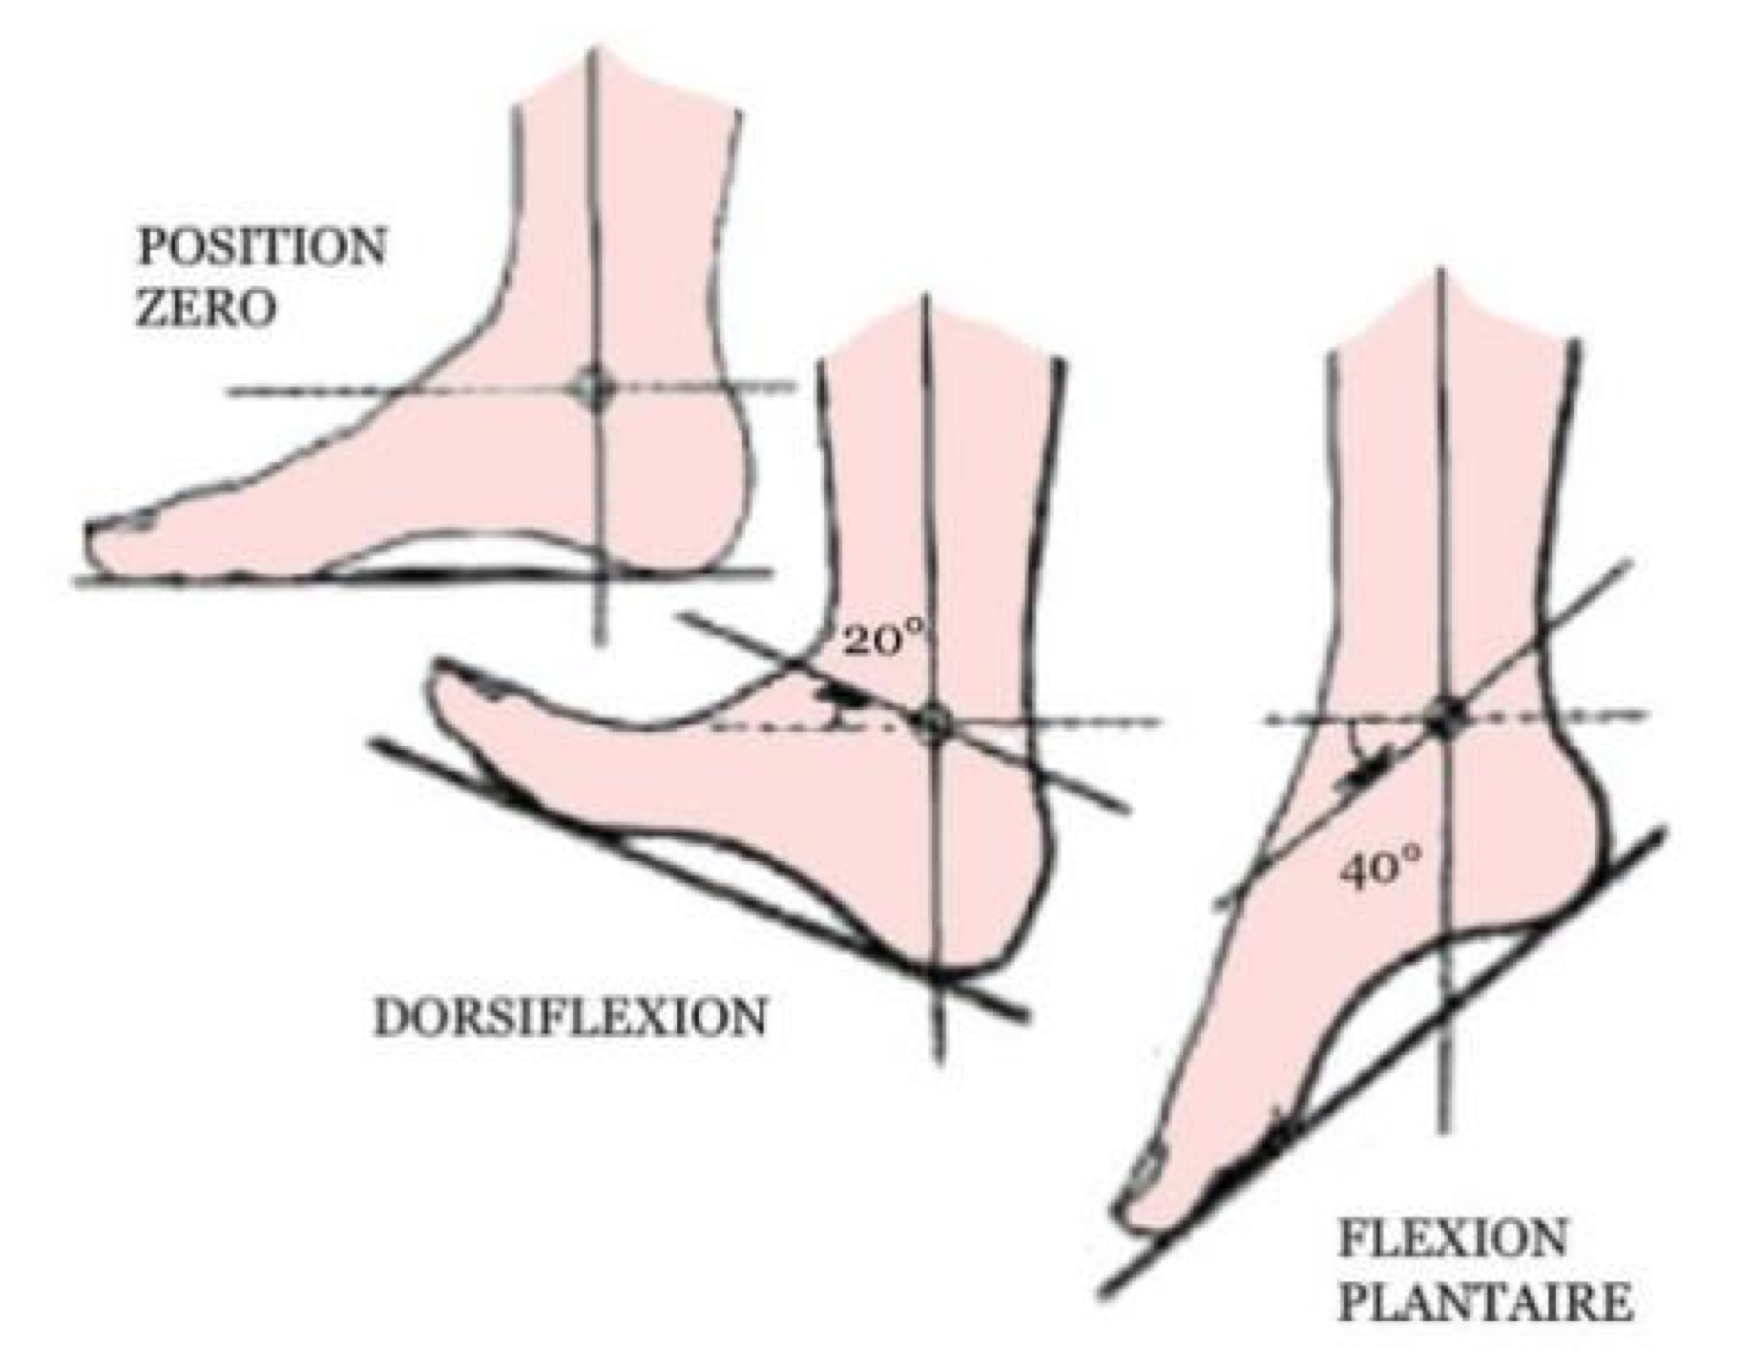
\includegraphics[height=4cm]{human_foot_sagittal.png}}
%     \hfil
%     \subfloat[][]{\label{fig:sagittal_trunk}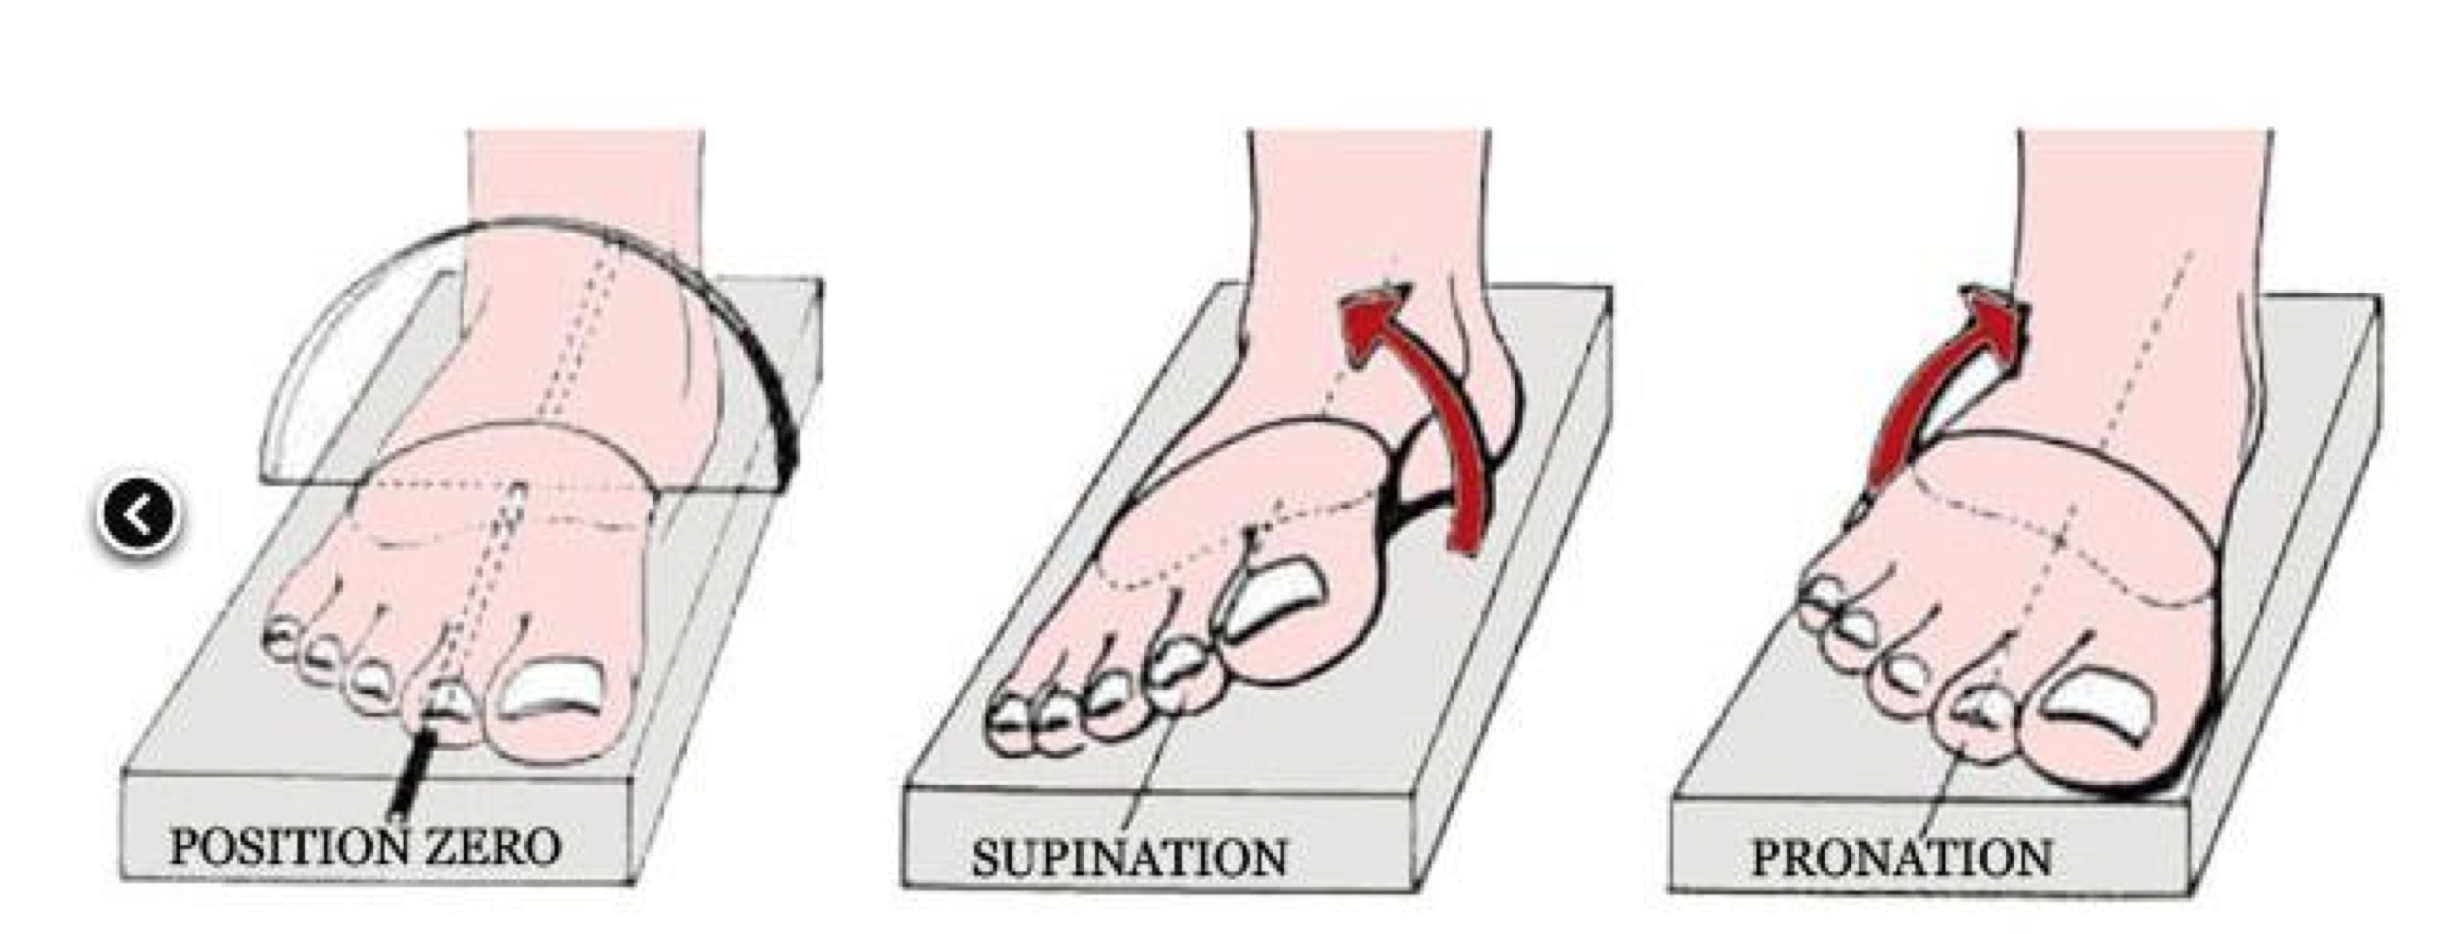
\includegraphics[height=3cm]{human_foot_lateral.png}}
%     \caption{}
%     \label{fig:poppy_torso}
% \end{figure}




\begin{figure}[p]
    \begin{center}
        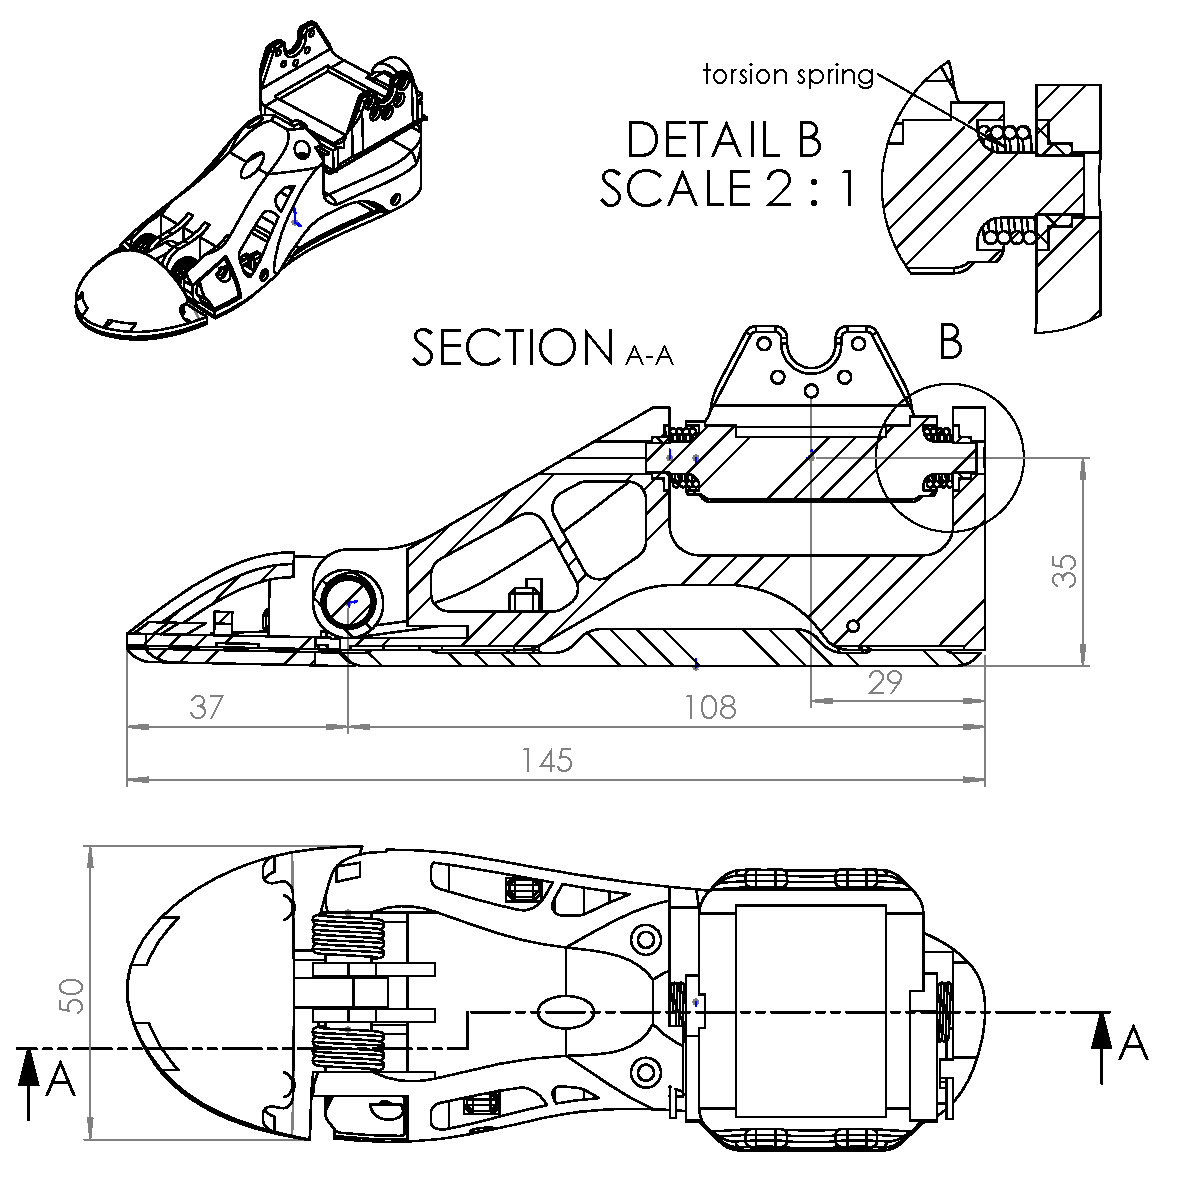
\includegraphics[width=\linewidth]{poppy_foot_v1.pdf}
    \end{center}
    \caption{}
    \label{fig:poppy-foot-v1-design}
\end{figure}


This design choice has a strong impact on the overall design, because we have lightweight feet, the power required to make the legs move is reduced, we can therefore use smaller motors which are also lighter.


\subsection{Legs} % (fold)

Poppy's legs have 6 DoF each, three on the sagittal plane (ankle, knee, hip), one on the horizontal plane (hip) and one on the frontal plane (hip). These joints allow reproduce the main DoF of the human legs. In addition, if we look closely at the morphology of the human femur, it appears that it is inclined by 6 degrees (see \figurename~\ref{fig:human_thigh}). This particularity is reproduced on Poppy's thigh (see \figurename~\ref{fig:poppy_leg_design}).

\begin{figure}[tb]
\centering
    \subfloat[][]{\label{fig:human_thigh}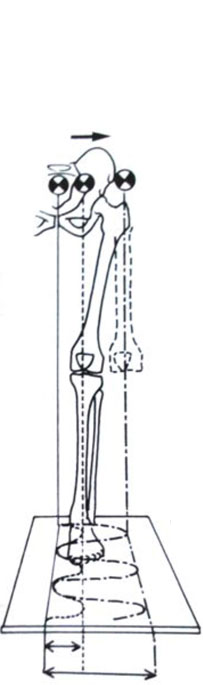
\includegraphics[height=6.5cm]{human_thigh.jpg}}
    \hfil
    \subfloat[][]{\label{fig:model_thigh}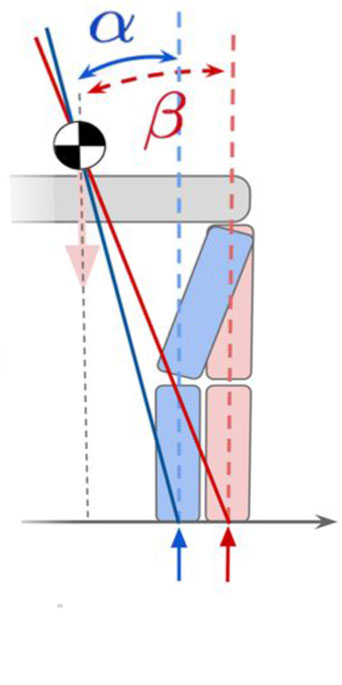
\includegraphics[height=6.5cm]{model_thigh.jpg}}
    \caption{ On \ref{fig:human_thigh}, effect of the bended femur on human biped locomotion. \ref{fig:model_thigh} Model used for the morphological comparison of the two thighs.}
    \label{fig:poppy_thigh}
\end{figure}


This slight bending makes the feet closer to the projection of the center of gravity and therefore changes the dynamic behavior.
In this thesis we describe both a theoretical model (see appendix REF) and real experiments (see section REF) showing that this bio-inspired thigh allows the reduction of falling speed by almost 60\% (during single support phase) and the decrease of the lateral motion needed for the mass transfer from one foot to the other by 30\% (double support phase).


\begin{figure}[p]
    \begin{center}
        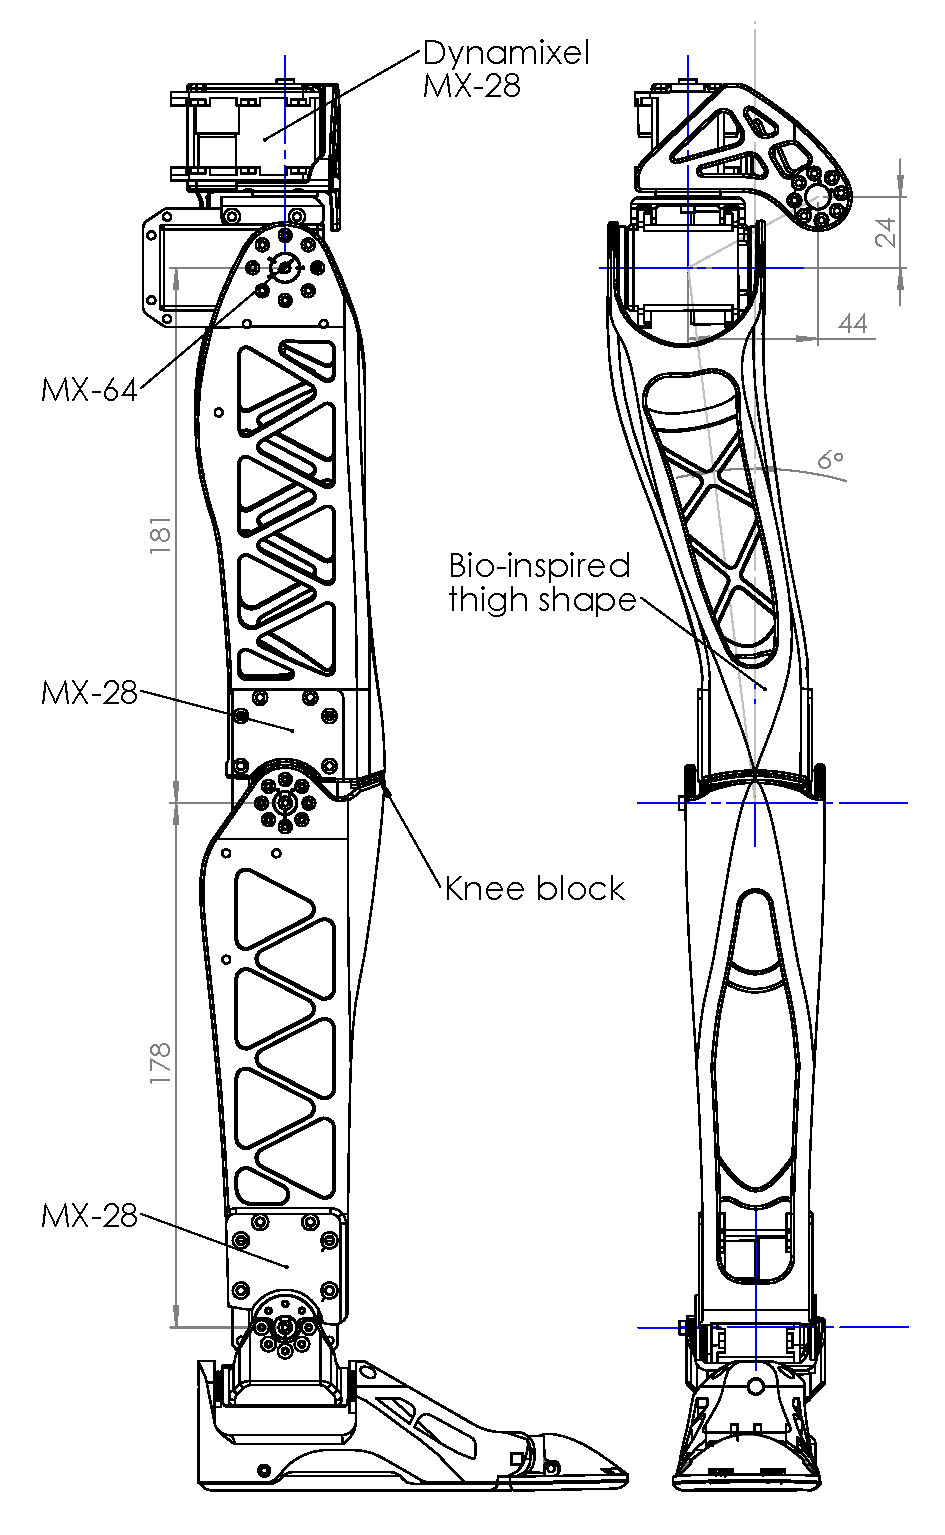
\includegraphics[width=\linewidth]{poppy_leg_design.pdf}
    \end{center}
    \caption{}
    \label{fig:poppy_leg_design}
\end{figure}


Also, following the principles previously mentioned, the leg design is made to be as light as possible. This was achieved by using truss structure (see section REF) and the minimum required amount of power, involving two Dynamixel MX-28 for the ankle and knee joint, and a Dynamixel MX-64 for the hip joint (see \figurename~\ref{fig:poppy_leg_design}). Yet as explained in section REF, most of our parts have several configurations allowing the actuator to be changed. Thus it is possible to easily replace the knee actuator by a Dynamixel MX-64 (see \figurename~\ref{REF}).



\section{Hip} % (fold)
\label{sec:hip}


Poppy's small feet increase the challenge of the balance of the robot. Also, to keep the projection of the center of gravity (CoG) inside the support polygon, defined by the feet geometry, it is necessary to control the weight distribution of the robotic structure. In particular, we wanted that in its initial upright posture, Poppy stays balanced without any control.

Robotis actuators are among the densest elements in the Poppy platform ($ 1700 kg.m^{3} $) and are the main source of weight ($1.8 kg$). Their spatial distribution represents therefore the major part of the distribution of mass in Poppy. In order to limit the displacement of the mass at the back of the robot, we decided to avoid a conventional ball joint assembly for the hip joint common on most robots based on Robotis motors such as DarwinOP or Acroban (i.e. distributed on a plane parallel to the sagittal plane). Instead, we placed them on the frontal plane as the left to right stability is greater than the rear to front stability. By doing so, the hip joint is not a real ball joint anymore. Yet to keep a wide range of motion, we used an original unsymmetrical motor configuration (see \figurename~\ref{fig:poppy_zoom_hip_blueprint}).

This configuration allows us:

\begin{itemize}
    \item to create a compact multi-articulated pelvis,
    \item have hip rotations (frontal plane) leading to slight vertical motions of the leg, which act as a damper during walking. This damping can be tuned by adjusting the stiffness of the actuator.
    \item to reduce the hip joint lever arm and thus reduce the torque required to maintain position in single support phase,
    \item to reduce the distance between rotation axes to stay close to a ball joint,
    \item the resulting V shape frees up room to increase the range of motion of the legs on both the frontal and horizontal plane.
\end{itemize}

\begin{figure}[p]
    \begin{center}
        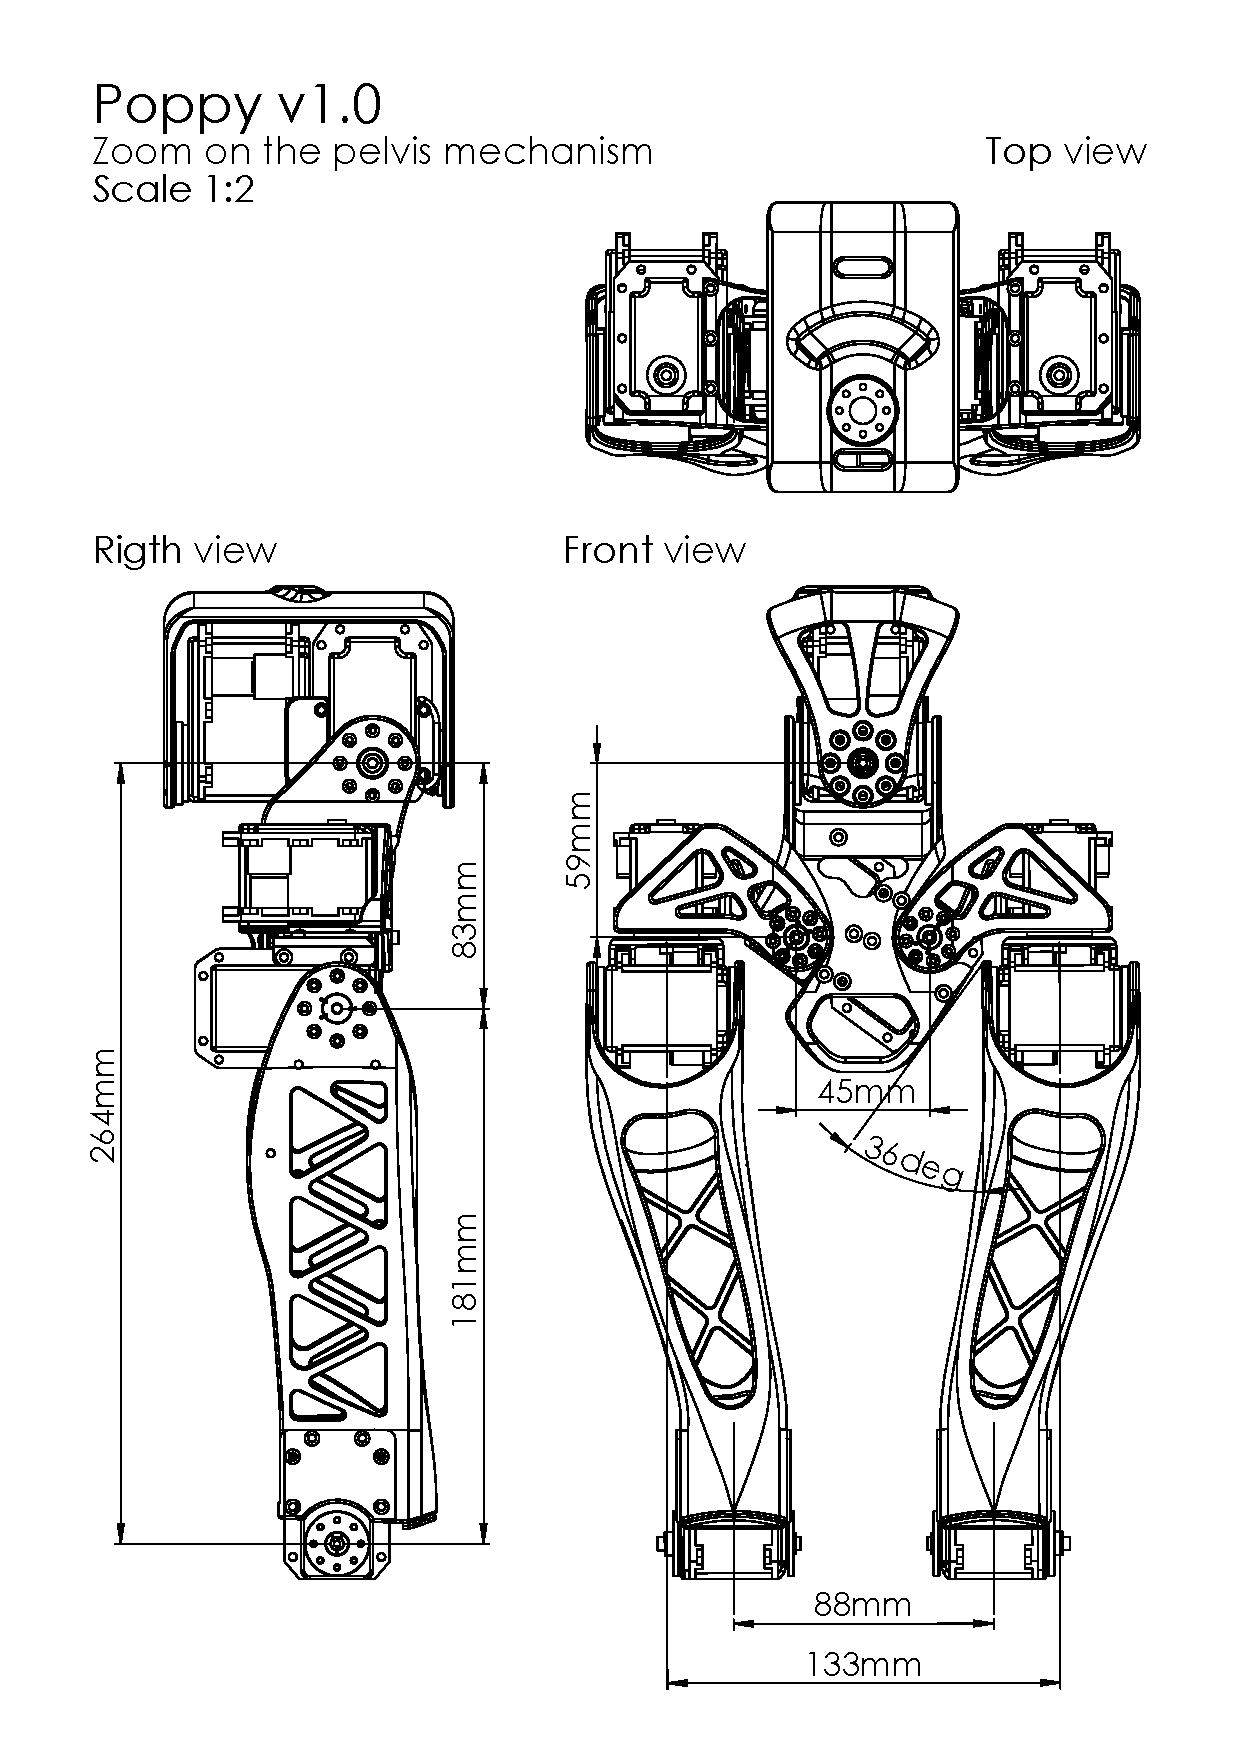
\includegraphics[width=\linewidth]{poppy_zoom_hip_blueprint.pdf}
    \end{center}
    \caption{}
    \label{fig:poppy_zoom_hip_blueprint}
\end{figure}

In addition, to reduce the shifting of the center of gravity to the back of the robot, the connection with the abs motors is slightly shifted toward the front. By doing so, we .
This enables us to keep the CoG within the support polygon and to increase the range of motion of the abs motor when the robot leans forward.


\section{Multi-articulated torso} % (fold)

Humanoid robots mostly have a rigid torso without any joints (e.g DarwinOp, Nao, NimbroOP) or few DoFs (e.g. two for Icub, one for HRP-2). However if we look at the human trunk and in particular at the spine, it has a complex mechanical structure and a large network of dense muscles controlling a very large number of DoFs. It allows for complex motions in several directions while keeping balance. Its movements are regulated by a complex combination of anticipatory and reactive muscle actions.

Before 1982 and the work of Thorstensson (58), few scientists had really approached the subject. Since then, several studies have investigated the activity of the trunk during walking, and showed that the trunk is not only an additional mass but for example, participates actively in the human walk.
Electromyographic studies have shown the importance of the erector spinae muscles in the organization of motor patterns during walking (61),(62),(63) but also of other rhythmic tasks (62). Like the salamander (8), a sequential activation of erector spinae muscles was found (64),(62).
They also show that the trunk leans forward and oscillates from 1.5 to 6 degrees during walking. In addition, lateral flexion during a gait cycle on the frontal plane promotes the weight shift and opposite rotations of the lumbar and thoracic belts on the horizontal plane allow for the extension of the footstep (59); (60).

\begin{figure}[ht]
    \begin{center}
        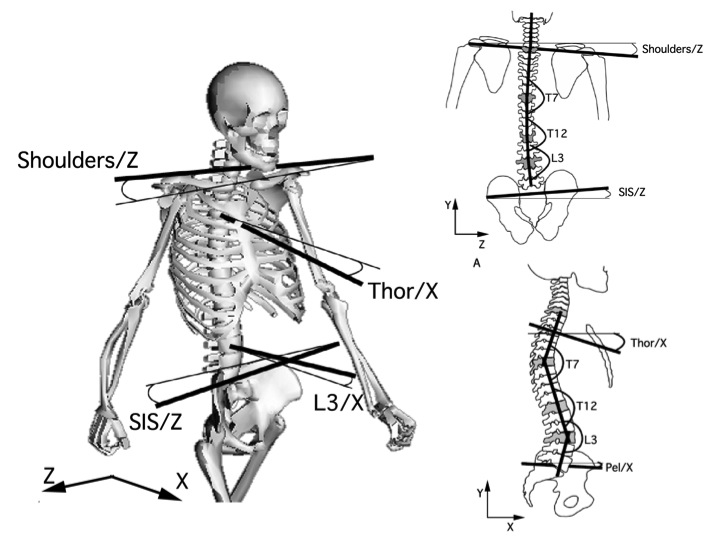
\includegraphics[width=0.7\linewidth]{human_trunk.jpg}
    \end{center}
    \caption{}
    \label{fig:human_spine_system}
\end{figure}

Thus the human torso is complex and seems to play an important role in walking; it is essential for all human movements but especially for walking. The movements of the spine can facilitate the transfer of weight from one leg to the other, improve the balance but also participate in the dynamics of walking.

It seems therefore interesting to equip a humanoid robot that is an attempt to explore the role of morphology, with an articulated trunk in order to evaluate its impact on several tasks, from dynamic walking to physical human-robot interaction. Yet the human torso is difficult to replicate on a small robot using servo motors and therefore simplification is needed.

Interestingly, Ceccato~\parencite{ceccatoPlos09} studied the role of the trunk during walking and highlighted that there are some places in the spine where the displacements are the most important, i.e. that the apparent high dimensionality of the trunk could be factorized down to a few essential components/dimensions.

Accordingly, it appears we can replicate the essential degrees of freedom of human torso with two DoFs on the sagittal plane, two on the coronal plane, placed in the pelvis and shoulder/thoracic and one on the horizontal plane placed in the middle of his torso.

These main degrees of freedom have been first introduced on Acroban~\parencite{ly2011bio} and continued on Poppy (see \figurename~\ref{fig:poppy_torso}).
Thus Poppy's trunk involves five degree of freedom, we use two Dynamixel MX-64 for the abs as they have to support and move the whole upper body mass, the 3 others joints being less subject to high constraints are powered by MX-28 (see \figurename~\ref{fig:torso_blueprint}). This multi-articulated trunk allows a wide range of motion that can be useful to explore the role of the torso’s motion on complex dynamics behavior (balance, walking), grasping and reaching task, or for human-robot interaction, extending to the expressive and emotional abilities.

\begin{figure}[p]
\centering
    \subfloat[][]{\label{fig:torso_blueprint}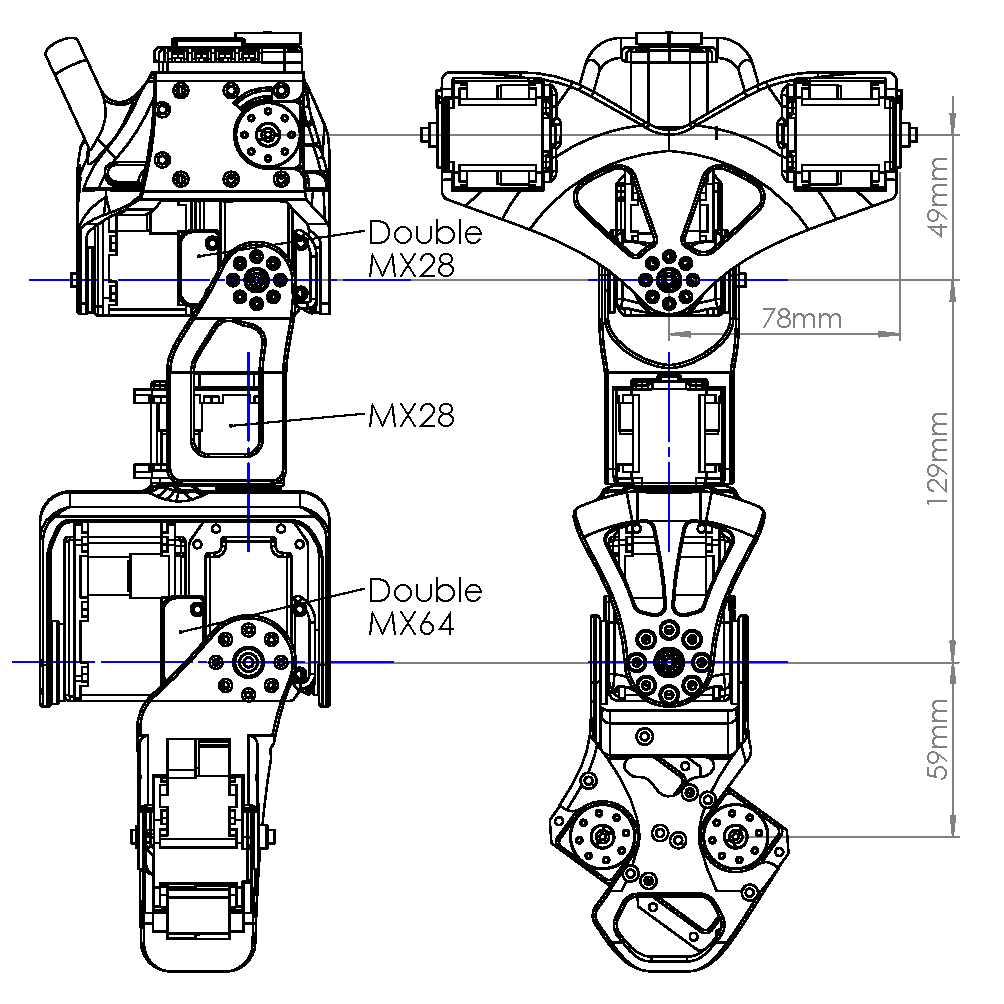
\includegraphics[width=0.95\linewidth]{poppy_torso.pdf}}


    \subfloat[][]{\label{fig:frontal_trunk}\includegraphics[width=0.48\linewidth]{trunk_face.png}}
    \hfil
    \subfloat[][]{\label{fig:sagittal_trunk}\includegraphics[width=0.48\linewidth]{trunk_sagittal.png}}
    \caption{These figures illustrate some morphological features of the Poppy humanoid Robot:\newline a) Poppy's limbs follow human proportions as described in~\parencite{dufour2005biomecanique}.\newline b) and c) Poppy has an articulated trunk of 5 DoFs which allows more natural and fluid motion while improving the user experience during physical interaction and actively participating in the balance of the robot.}
    \label{fig:poppy_torso}
\end{figure}



\subsection{Upper limbs} % (fold)

Poppy's arms were not designed for exploring grasping but rather for balancing, expressive and interactive purposes. Thus they only involve the minimum articulations required to produce a wide range of movements and they do not involve articulated hands.

A first version of the robot arms involved low-cost AX-12 motors(\$50), but these motors do not allow the same degree of compliance as MX-28 so the interaction was not smooth enough. We quickly replaced them with MX-28 motors, even if they are more expensive (\$250), powerful and heavy (72gr rather than 50gr), the compliance ability is needed for playful physical interaction and demonstration.

This ability was especially useful for the experiments we made with Poppy walking while being socially guided by its hands see videos\footnote{} and experiments on section REF.

Thanks to its multi-articulated structure and its expressive head,

Also these arms combined with the complex spine make Poppy a particularly adapted tool for creating and studying emotions and gestural social communication (see \figurename~\ref{fig:TER_cognitic}). An example of such use has been demonstrated by two cognitivist students. Their goal was to study the transfer of emotion between robots and humans. Using Poppy's upper body and the pypot recording feature (see section REF), they were able to program a wide range of emotions (see \figurename~\ref{fig:TER_cognitic}).


\begin{figure}[tb]
\centering
    \subfloat[][\url{http://youtu.be/StFIMuyz11M}]{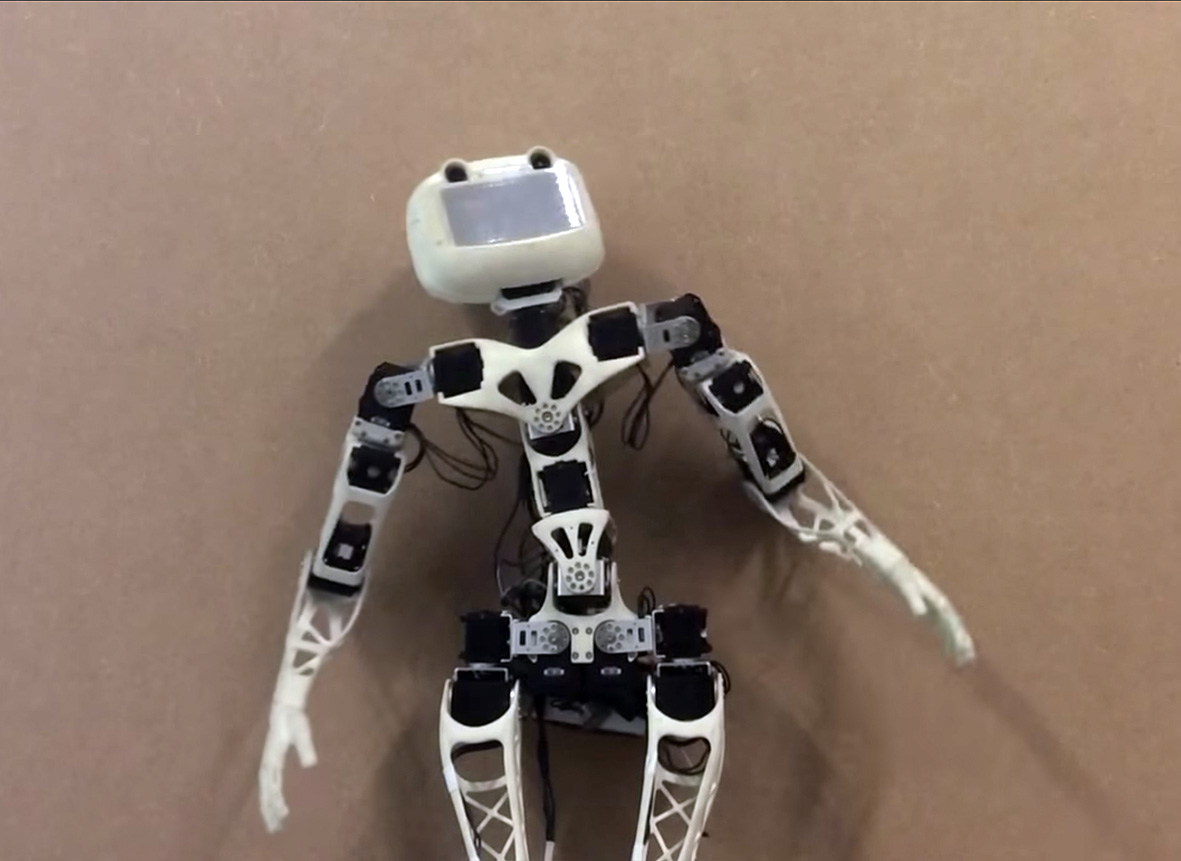
\includegraphics[width=0.45\linewidth]{TER_surprise.jpg}}
    \hfil
    \subfloat[][\url{http://youtu.be/RwCtNwLk10E}]{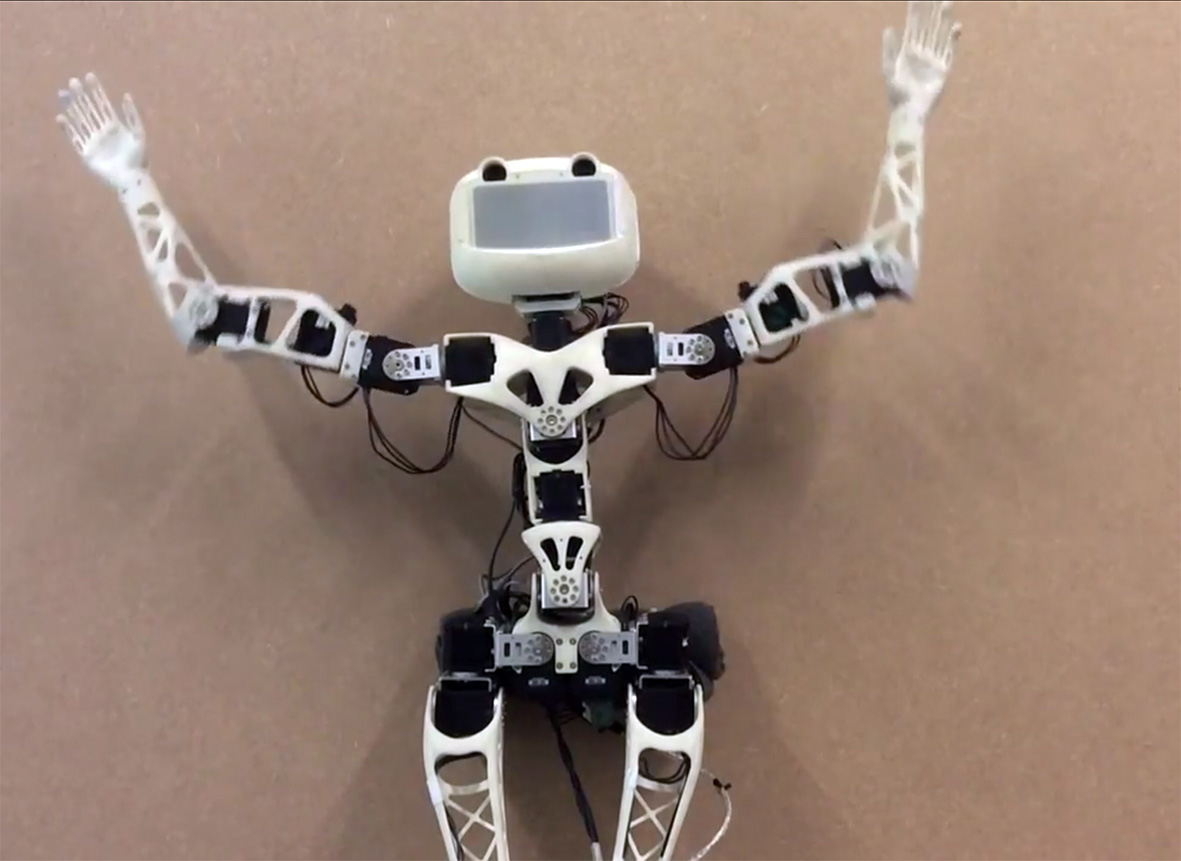
\includegraphics[width=0.45\linewidth]{TER_joy.jpg}}\\
    \subfloat[][\url{http://youtu.be/qrcmLXbpUVo}]{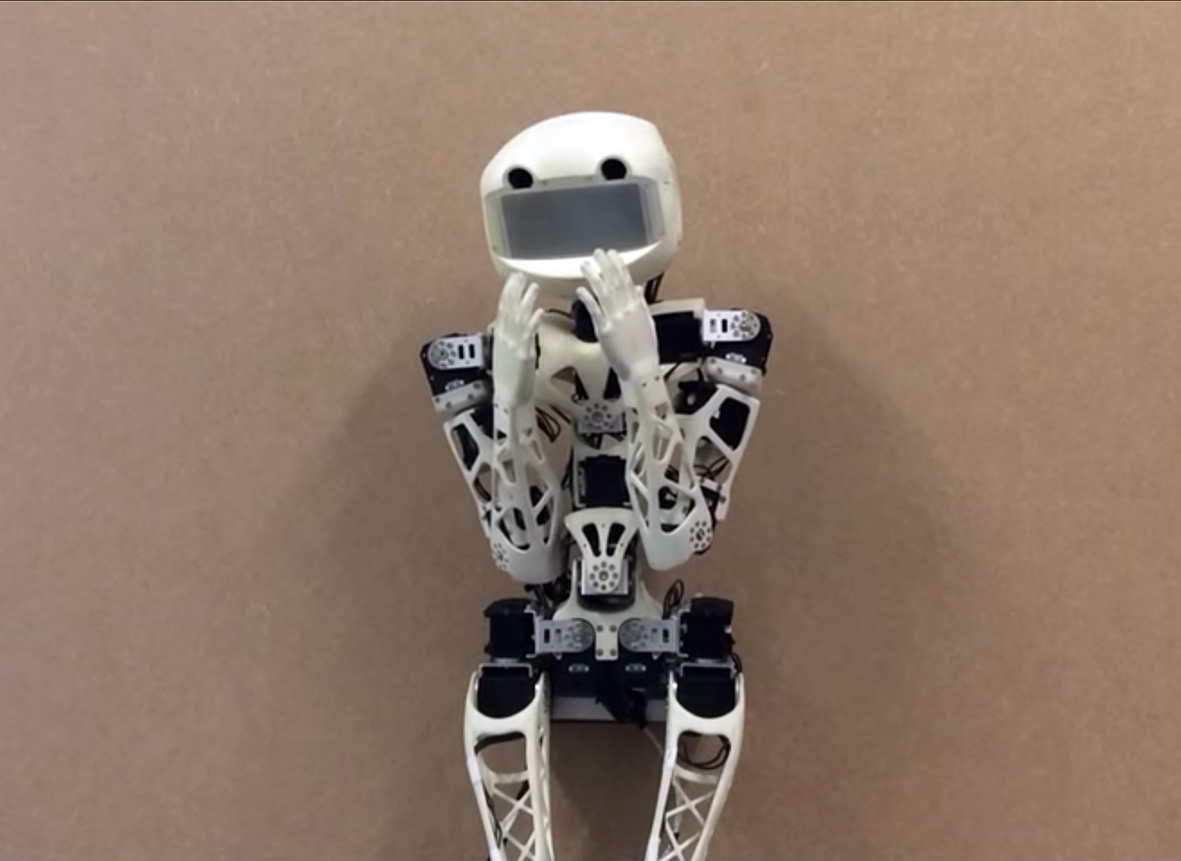
\includegraphics[width=0.45\linewidth]{TER_sad.jpg}}
    \hfil
    \subfloat[][\url{http://youtu.be/ms2niFLevv8}]{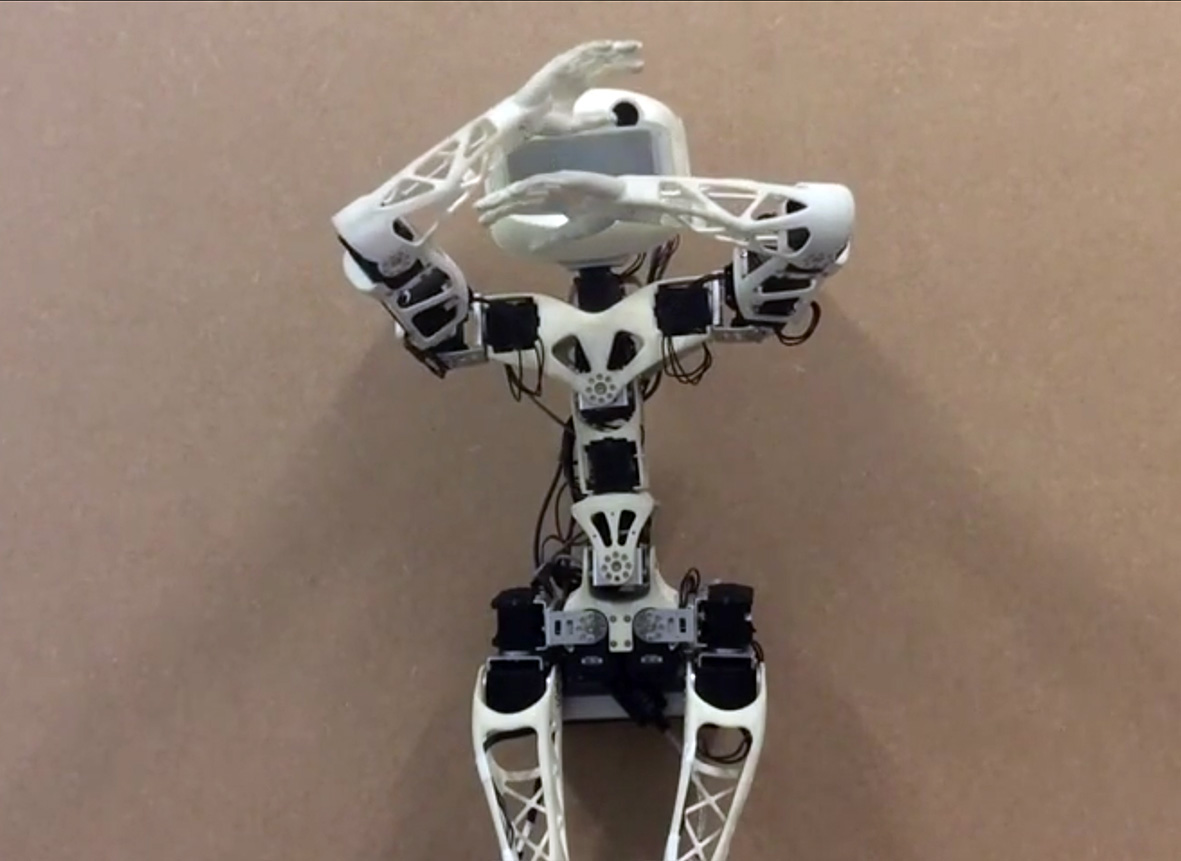
\includegraphics[width=0.45\linewidth]{TER_fear.jpg}}
    \caption{}
    \label{fig:TER_cognitic}
\end{figure}



% !TEX root = ../../thesis.tex

\section{Electronic architecture} % (fold)

To keep the spirit of the project described by its guidelines (see previous section REF), the electronic architecture has to be simple, easily reproducible, relatively low-cost and modular. Of course the performance of each components is very important and should be correctly dimensioned.

The first version of Poppy (beta) had a handmade electronics architecture, which required hacking several components before soldering them together. This design was not compliant with the design guidelines of Poppy (i.e. easy to use and to reproduce) and was actually the main reason Poppy was considered as a beta version. Recent work has been done toward the simplification and the reproducibility of the electronics part.

Yet the electronic integration is challenging. Indeed, because Poppy has 5 degrees of freedom in the torso, there is not enough room for all electronic components needed. Therefore we had to embed most of them in the head which raise a room problem but also a mass problem.


Poppy's electronic architecture is based on several key-components communicating with each other (see Figure Ref):
\begin{itemize}
    \item an IO board controlling all the sensorimotor space,
    \item an embedded computing module to permit wireless communication,
    \item a head screen to display emotions or information,
    \item an alimentation board to provide the 12V needed for the motors and 5V needed for electronic systems,
\end{itemize}

\begin{figure}[tb]
    \begin{center}
        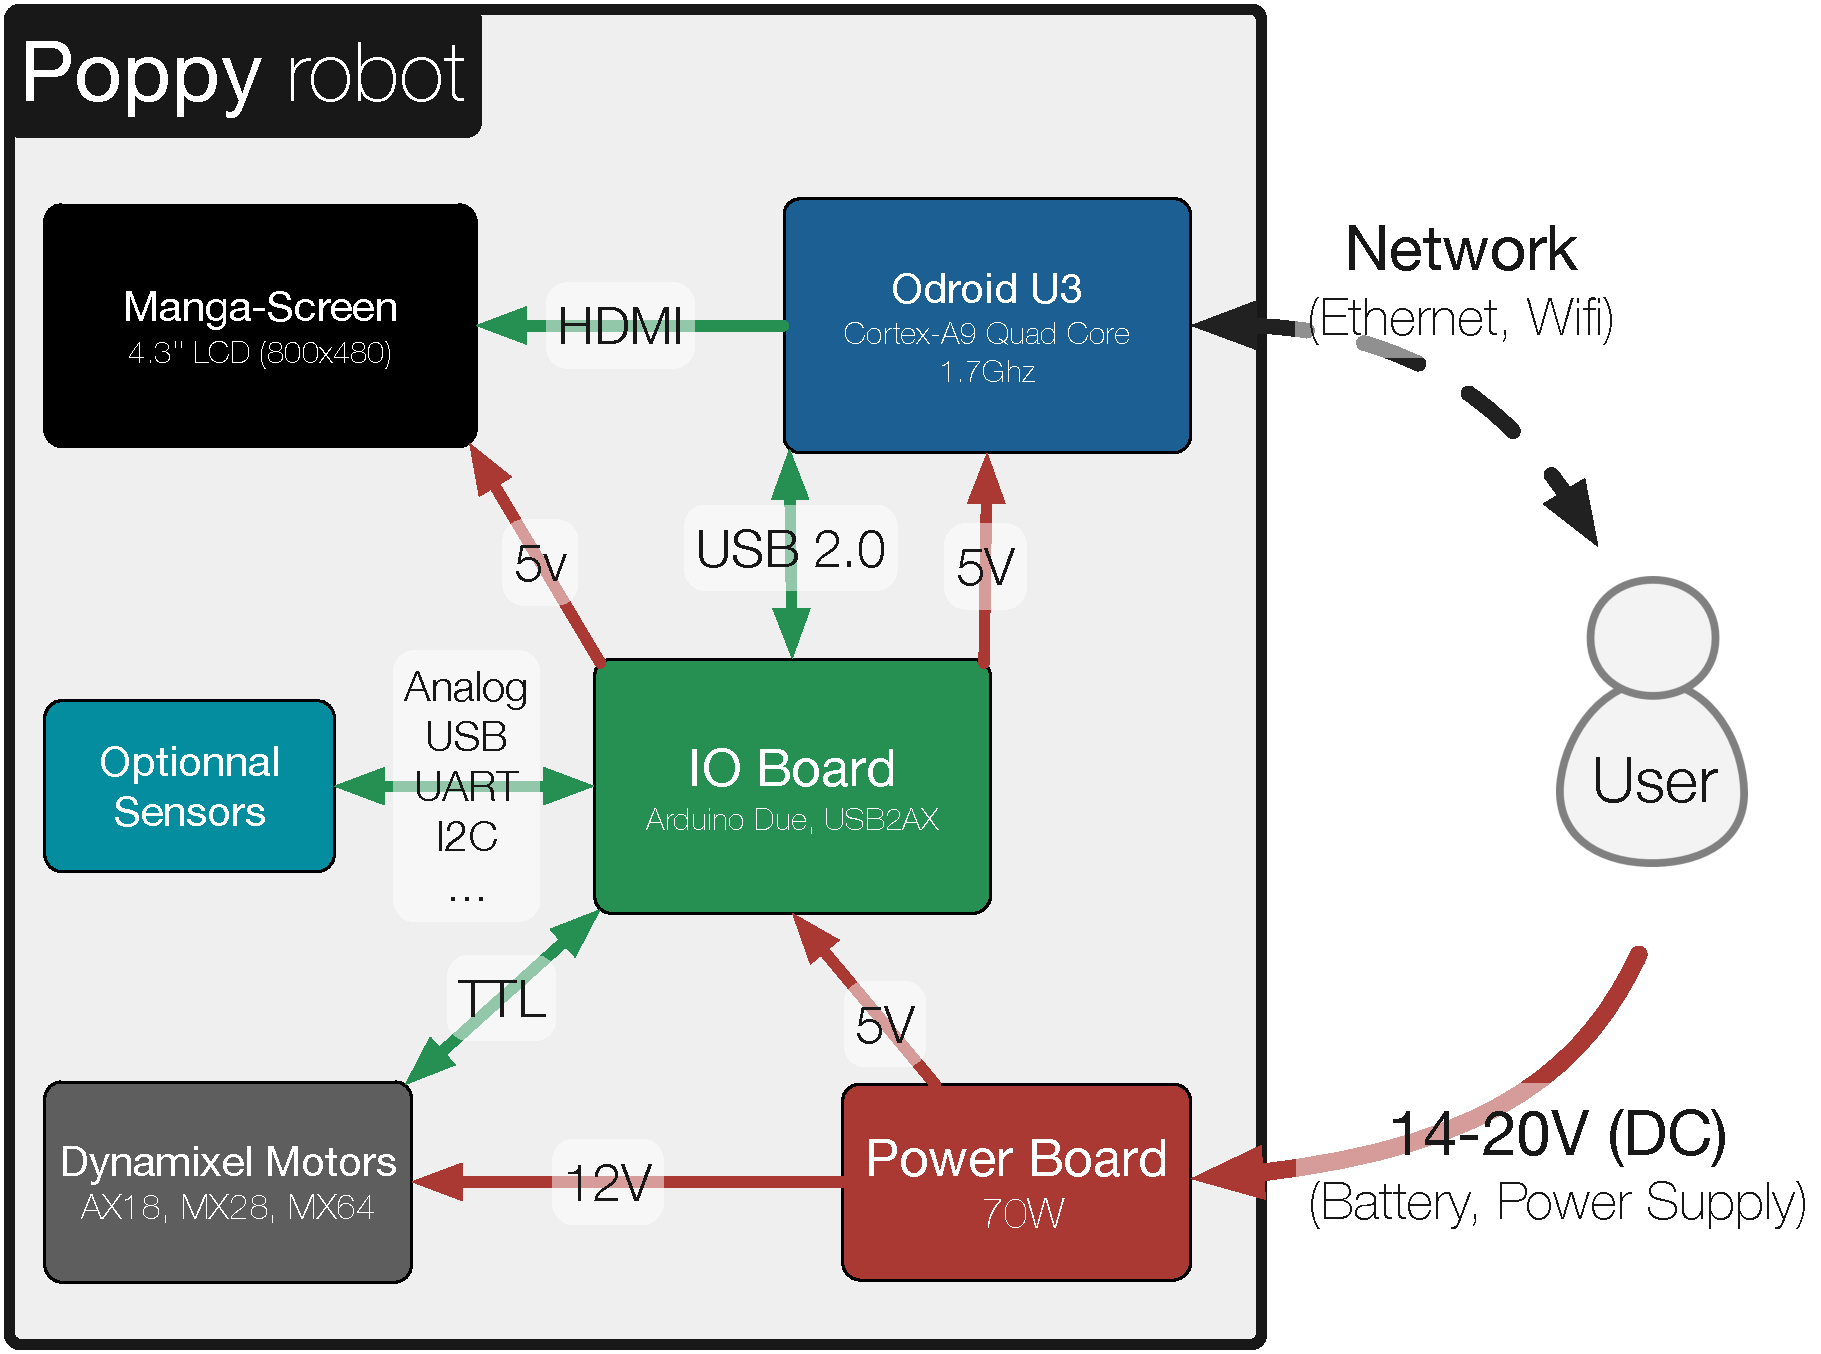
\includegraphics[width=\linewidth]{poppy_electro_archi_overview.pdf}
    \end{center}
    \caption{Caption here}
    \label{fig:figure1}
\end{figure}

We will discribe in this section, the design choices we made for this several components.

\subsection{Poppy IO Board} % (fold)

With the aim to offer easy-to-use modular electronics architecture and to make it fit in the head of Poppy, we decided to create a custom board. We could argue it makes more complex the diffusion of the platform while a custom board is too complex to be handmade and should therefore follows the industrialization process we are trying to avoid since the early age of the project. Nevertheless the makers revolution brings novel solutions to produce electronics. Indeed, there are now companies (such as CircuitHub\footnote{\url{https://circuithub.com}}), which offer scalable solution tools from 1 sample to a 10,000 batch. It is possible to upload our design and anyone can ask to make it produced. Of course ordering one part is more expansive but stay relatively low compare to the robot cost.

The board we designed included the basic element needed both for the control of the robot and for its extensibility.


\subsubsection{Motor control} % (fold)
Robotis Dynamixel are normally controlled by the \emph{USB2Dynamixel} but we decided to replace it by USB2AX devices (see \figurename~\ref{fig:usb2ax}). The USB2AX is a small interface to control Dynamixel servomotors from a computer and designed by Nicolas Saugnier. It plugs into a USB port and has a 3-pin molex connector compatible with the robotis ones.

For the use in Poppy, these devices has several main advantages:
\begin{enumerate}
    \item They are a lot smaller than the standard USB2Dynamixel module (16x36mm instead of 35x90mm) (see \figurename~\ref{fig:USB2AX_vs_USB2Dxl}).
    \item They can endure a short-circuit between the DATA and power-supply wire.
    \item They have the sync\_read instruction to read a lot of information very fast, which is not a standard Dynamixel instruction. The USB2AX converts SYNC\_READ into multiple separate READ commands to get data from each servo, then sends back to the computer a single big packet containing all the data. This significantly decreases the effect of USB latency. A SYNC\_READ command reads the same registers in each servo (see \figurename~\ref{fig:usb2ax-perf}).
    \item It is open source so we can extend or adapt this solution to our needs.
\end{enumerate}

\begin{figure}[tb]
\centering
    \subfloat[][]{\label{fig:usb2ax_dongle}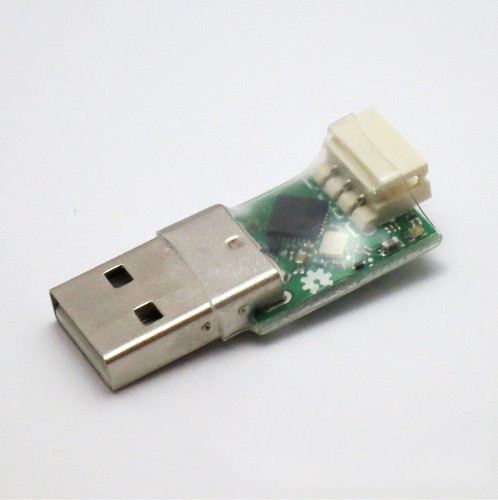
\includegraphics[height=4.5cm]{usb2ax.jpg}}
    \hfil
    \subfloat[][]{\label{fig:USB2AX_vs_USB2Dxl}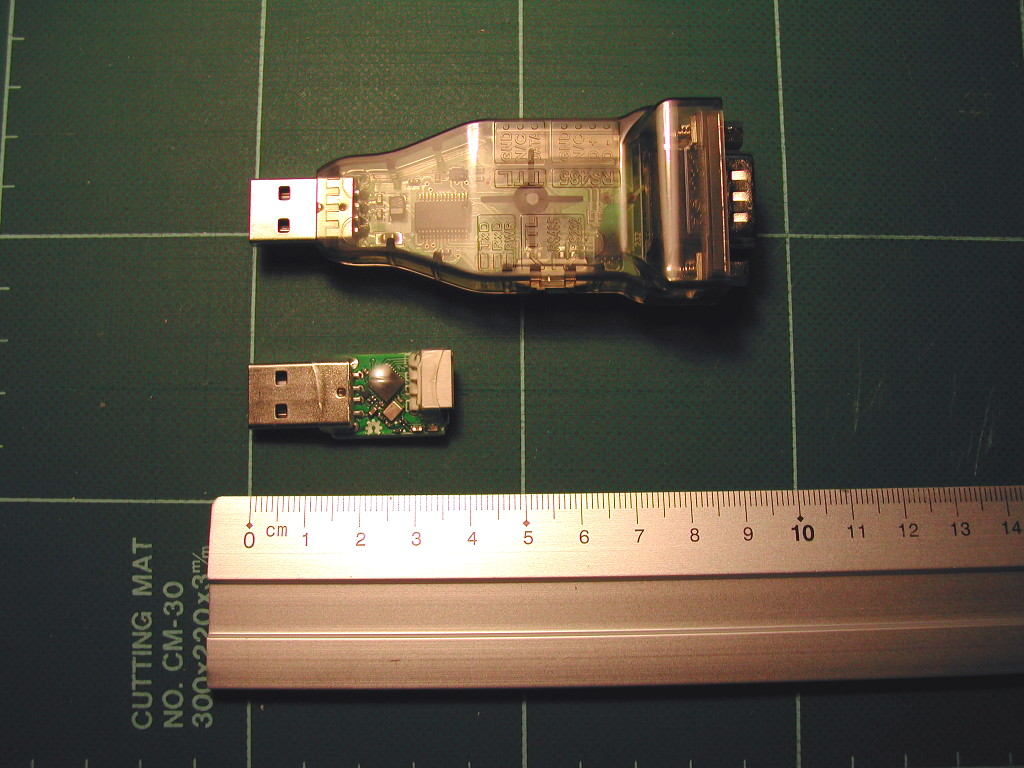
\includegraphics[height=4.5cm]{USB2AX_vs_USB2Dxl.jpg}}\\

    \subfloat[][]{\label{ig:usb2ax-perf}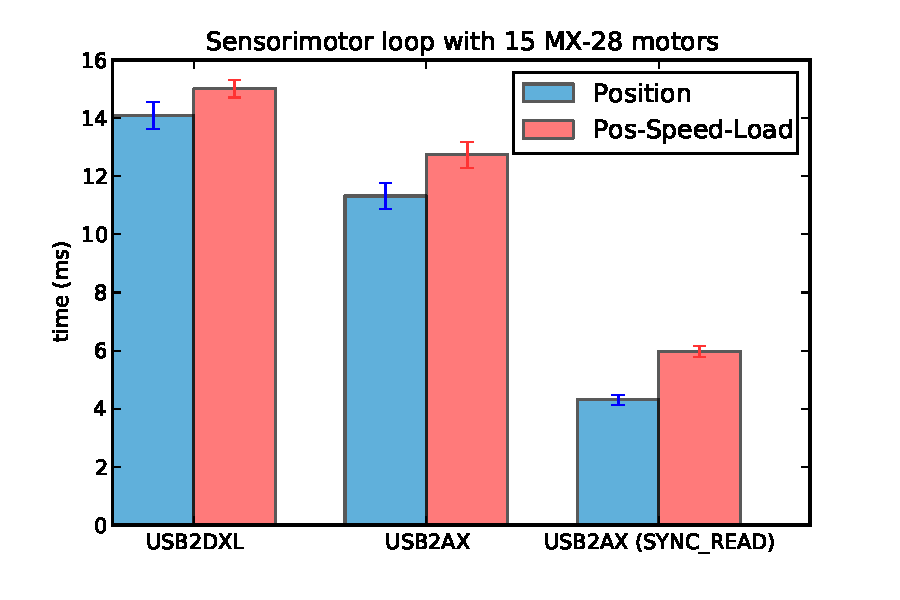
\includegraphics[height=5.5cm]{motor-bench.pdf}}
    \caption{}
    \label{fig:usb2ax}
\end{figure}

This project has always been used on Poppy and greatly help us to both have a effective robot while keeping the room for electronic low.
Because the project is open hardware, we could have reuse it to embed it directly on a custom board so we can make it even smaller by avoid usb connectors.

\subsubsection{Arduino integration} % (fold)
As we explain in the section REF, the modularity of the Poppy electronics is achieved thanks to the use of the Arduino environment. For the Arduino integration we decided to use the new Arduino Due based on the Atmel SAM3X8E ARM Cortex-M3 CPU. These board embeds both a powerful microcontroller (84 MHz 32-bit ARM core) and a large number of inputs/ouputs: 54 digital input/output pins (of which 12 can be used as PWM outputs), 12 analog inputs, 4 UARTs (hardware serial ports).


\subsubsection{Actual design of the IO Board} % (fold)
The IO board is an open hardware project aiming to simplify the use of Poppy for non-electronic-expert users. Therfore it integrates into one board all components it would be necessary to plug or solder.


This board is based on the other open hardware projects previously presented and contains two usb2ax for communication with Robotis actuators, an Arduino Due to permit the extension of the sensors space plus convenient  ports to easily plug external devices. See \figurename~\ref{tab:io-board-specs} for a complete details of all the available IO ports.

In addition, it integrates two sensors: a ADXL345 accelerometer, which has four measurement range (2g/4g/8g/16g) with up to 13-bits resolution and a data rate up to 3200Hz; and a ITG-3200 gyroscope, which has a full scale range of +/- 2000\textsuperscript{o}/s with 16-bits resolution and data rate up to 36kHz.


The board has been designed using KiCad\footnote{Open source EDA software}, the source are distributed under open source license\footnote{Creative Commons CC-BY-SA} and aivailble on our GitHub project\footnote{\url{https://github.com/poppy-project/poppy-electronics/tree/master/CarteIo}}. The production of the board can be done using CircuitHub\footnote{\url{https://circuithub.com/projects/Poppy_project/CarteIo}} and costs \$250 for one board or \$90 for ten\footnote{The cost descrease with quantity up to \$50.}.

\begin{figure}[p]
\centering
    \subfloat[][]{\includegraphics[width=\linewidth]{IO_Board.pdf}}


    \subfloat[][]{\label{tab:io-board-specs}
        \begin{tabularx}{0.8\linewidth}{r X}
        \textbf{2x} & high-speed motors buses\\
        \textbf{2x} & UART ports\\
        \textbf{1x} & I2C bus\\
        \textbf{2x} & external USB Ports\\
        \textbf{1x} & accelerometer\\
        \textbf{1x} & gyroscope\\
        \textbf{12x} & anlog pins\\
        \textbf{12x} & digital pins allowing PWM control\\
        \textbf{4x} & 5v ports to supply power to external devices\\
        \end{tabularx}
        }
    \caption{}
    \label{fig:IO-board}
\end{figure}


\subsection{Embedded computing module} % (fold)

The integration of a computing module is rather complex and not fundamental if the robot cannot walk for more than 5m, therefore the Poppy beta version was controlled using an external computer connected by USB.
However Poppy aims to become a shared research platform with people adressing challenge in which the embeded control can be necessary. Also as all user have a different computer configuration (Windows, MacOS and the plenty of Linux distribution), it is easier to maintain the control software if only one OS is used. Embedding a linux allows to have the control and ensure same performance for every Poppy.

Yet as I said previously, embedding control is complex. Indeed, the computer has to be small enough to fit inside the robot. With such size, where are mostly ARM based computer. Most of work are developed on x86 or 64 architecture and the switch to ARM architecture is not direct. Some software module used does not exist or are not optimized leading to big performance problems.

It is the case with one of the most famous micro-computer, the raspberry pi. The first trials we made using Pypot was really disappointing on the performance aspect. As we can see in section REF, it takes about 10-12 ms just to read and write a motor position (mostly computing) while it is only 2ms on a normal computer (mostly serial communication). Therefore we oriented our choice toward the Hardkernel Odroid U3 board (8\~12 times faster than the Raspberry Pi).

\begin{figure}[p]
    \centering
    \subfloat[][]{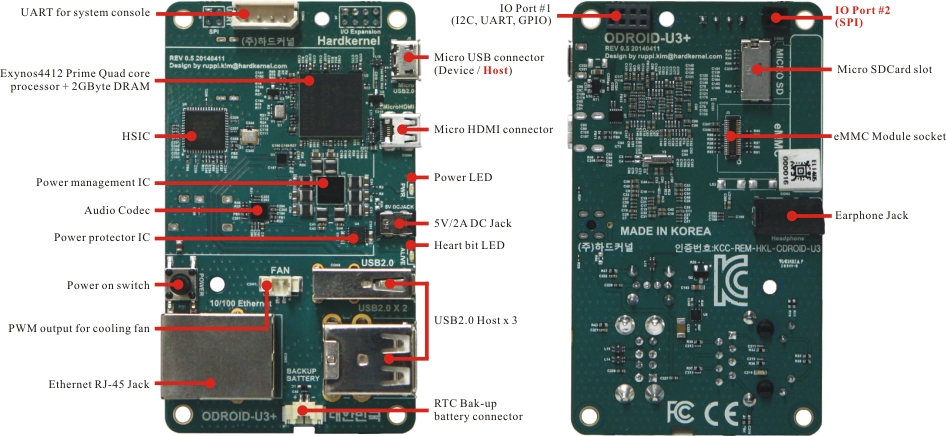
\includegraphics[width=\linewidth]{Odroid_U3.jpg}}


    \subfloat[][]{\begin{tabularx}{\linewidth}{r X}
        % \hline
        \textbf{Processor} & Samsung Exynos4412 Prime Cortex-A9 Quad Core 1.7Ghz with 1MB L2 cache\\
        \textbf{Memory} & 2048MB(2GB) LP-DDR2 880Mega data rate\\
        \textbf{3D Accelerator} & Mali-400 Quad Core 440MHz\\
        \textbf{Video} & supports 1080p via HDMI cable(H.264+AAC based MP4 container format)\\
        \textbf{Video Out} & micro HDMI connector\\
        \textbf{Audio} & Standard 3.5mm headphone jack HDMI Digital\\
        \textbf{LAN} & 10/100Mbps Ethernet with RJ-45 Jack ( Auto-MDIX support)\\
        \textbf{USB2.0 Host} & High speed standard A type connector x 3 ports\\
        \textbf{USB2.0 Device} & ADB/Mass storage(Micro USB), Host mode is possible if the PCB Rev is 0.5 or higher.\\
        \textbf{Display} & HDMI monitor\\
        \textbf{IO Port} & GPIO, UART, I2C, SPI(Board Revision 0.5 or higher)\\
        \textbf{Storage (Option)} & MicroSD Card Slot eMMC module socket\\
        \textbf{Power (Option)} & 5V 2A Power\\
        \textbf{System Software} & Linux : Xubuntu 13.10 or latest version Android : u-boot 2010.12, Kernel 3.0.x, Android 4.x  Full source code is available now.\\
        \textbf{PCB Size} & 83 x 48 mm\\
        \textbf{Weight} & 48g including the heat sink\\
         & \\
        % \hline
        \end{tabularx}
        }
    \caption{Hardkernel Odroid U3 computer board}
    \label{fig:odroid_U3}
\end{figure}

The Hardkernel Odroid U3 (see \figurename~\ref{fig:odroid_U3}) is a low-cost (\$65) and powerful Linux computer embedding a 1.7GHz Quad-Core processor and 2GByte RAM while being very small (83 x 48 mm) and lightweight (48 grams) (see Tab.~\ref{tab:table_feet} for the detail of all specifications).


Among the plug-n-play small computers, the Odroid U3 is currently the most suitable board for our application according to the size, the computing power and the I/O positions.
Yet as we will explain in the limitations (see section REF), this solution is still not perfectly satisfying and the use of plug'n'play computer raises a lot of integration problem.

\subsection{Display} % (fold)

The video out port on all new mini computer boards such as Raspberry Pi, Beagle board or Odroid boards is HDMI port. Finding small screen (< 7inch) compatible with HDMI input is really hard and currently only one project exists.The manga-screen (see \figurename~\ref{fig:manga-screen}) is a open source (CC-BY-SA\footnote{see REF}) multi purpose, HDMI compatible LCD screen. This board is developed by Elias Bakken and works with a 4.3 inch screen (480x800px) made by Sharp\footnote{Sharp LQ043Y1DX07}.

\begin{figure}[h]
\centering
    \subfloat[][]{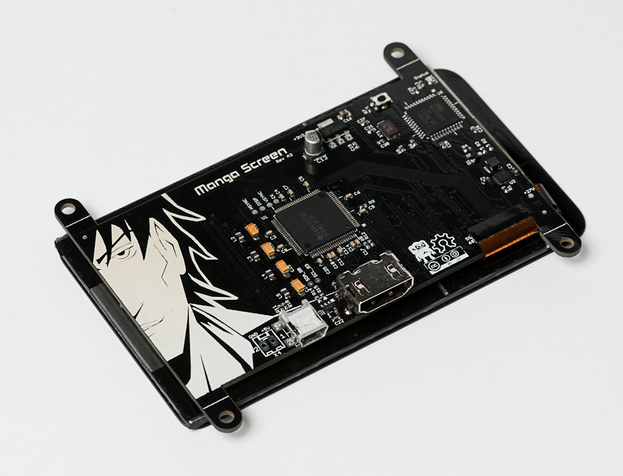
\includegraphics[height=4.9cm]{manga-screen.png}}
    \hfil
    \subfloat[][]{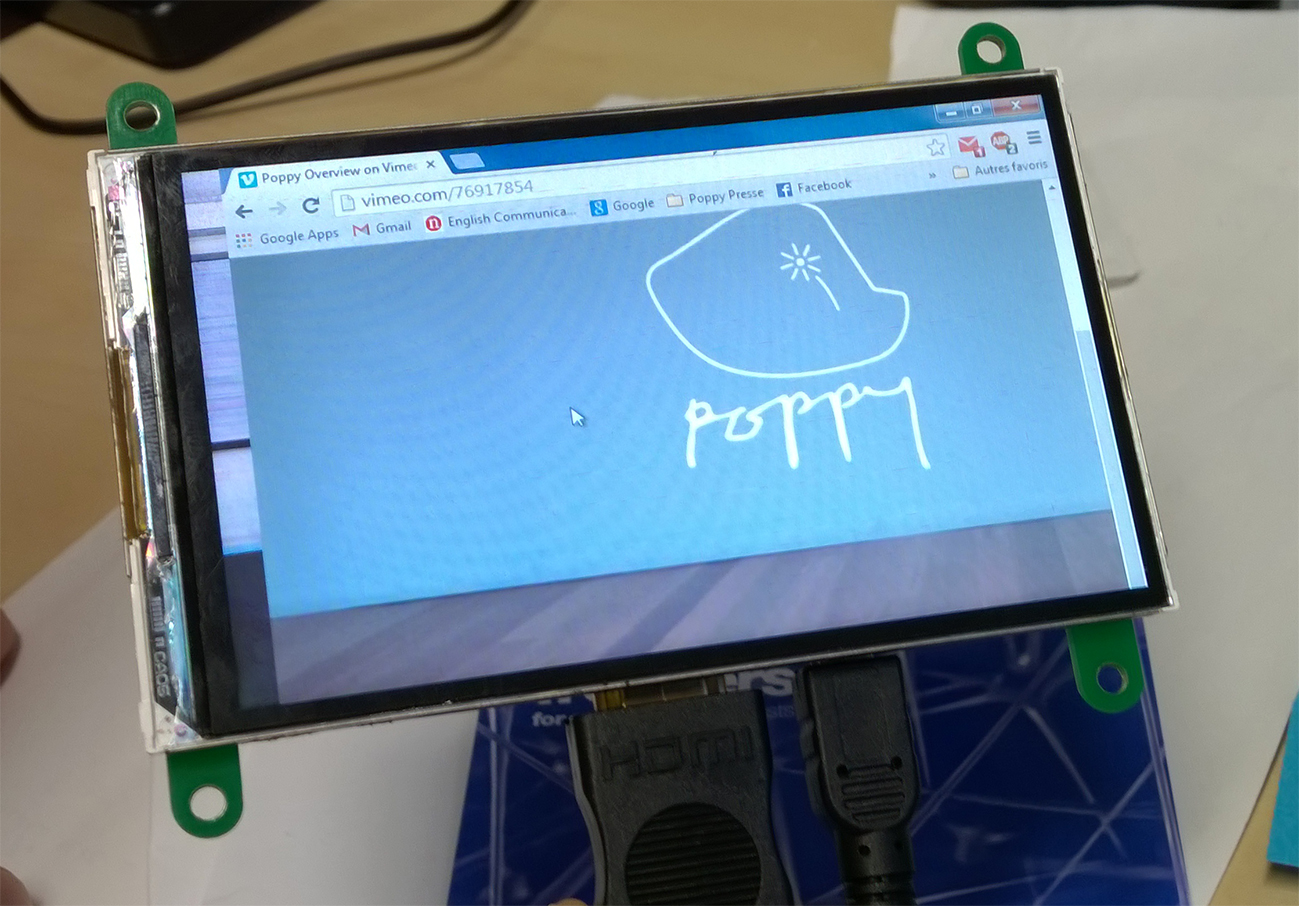
\includegraphics[height=4.9cm]{poppy_screen.jpg}}
    \caption{}
    \label{fig:manga-screen}
\end{figure}

The integration of a led matrix panel would be easier but it would require to create driver for the display.
Using a HDMI display connected to a Linux computer allows user to easily display information or animation on the screen like if it was on their monitor. Therefore users are free to use any tools they like such as Processing, OpenGL, VLC or whatever. This flexibility would not be possible with a matrix led panel which would have required to control the information displayed with Arduino programming.

\subsection{Alimentation} % (fold)
\label{ssub:alimentation}

\subsubsection{Power board} % (fold)
The current Poppy's alimentation is ensured by Robotis power supply. This solution is really low-cost with a dozens of euros but it is limited. Indeed, the Robotis power supply provides directly 12V@5A dans is plugged directly on the robot. Yet the wire is short and not really convenient. It would be a better solution to have on board active components allowing to convert a wide range of power supply to the one needed for Poppy. In particular, we could be compatible with standard laptop power supply (18-22V).

This work is still in progress and the chosen solution will be presented in the final version of this thesis.


\subsubsection{The battery issue} % (fold)

An issue associated with the batteries is the mass. Indeed 3.6V battery cell weights around 45 grams and we need at least 4 cells to supply the 12V needed for Poppy, thus a 14,4V pack weights almost 200 grams (see \figurename~\ref{fig:battery_specs}). For comparison a MX-28 Dynamixels weights 72grams so a battery pack suitable for Poppy weigths approximately the same mass as 3 motors.
In addition, the overall size is quite big with 18mm x 65mm x 18mm (see \figurename~\ref{fig:battery_size}) and makes the integration complicated in a multi-articulated and small robot like Poppy.

Poppy is not yet able to walk by itself, being energtically autonomous does not seem a high priority. Thus we chose to not include battery in the current Poppy electronic architecture. Yet, we hope community will try to address this challenge and maybe find original and suitable solutions.

\begin{figure}[tb]
\centering
    \subfloat[][]{\label{fig:battery_size}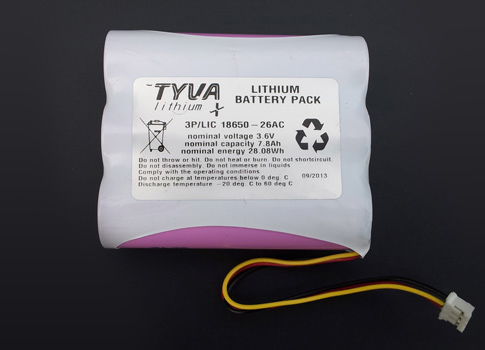
\includegraphics[height=3.5cm]{tyva_battery_pack.jpg}}
    \hfil
    \subfloat[][]{\label{fig:battery_specs}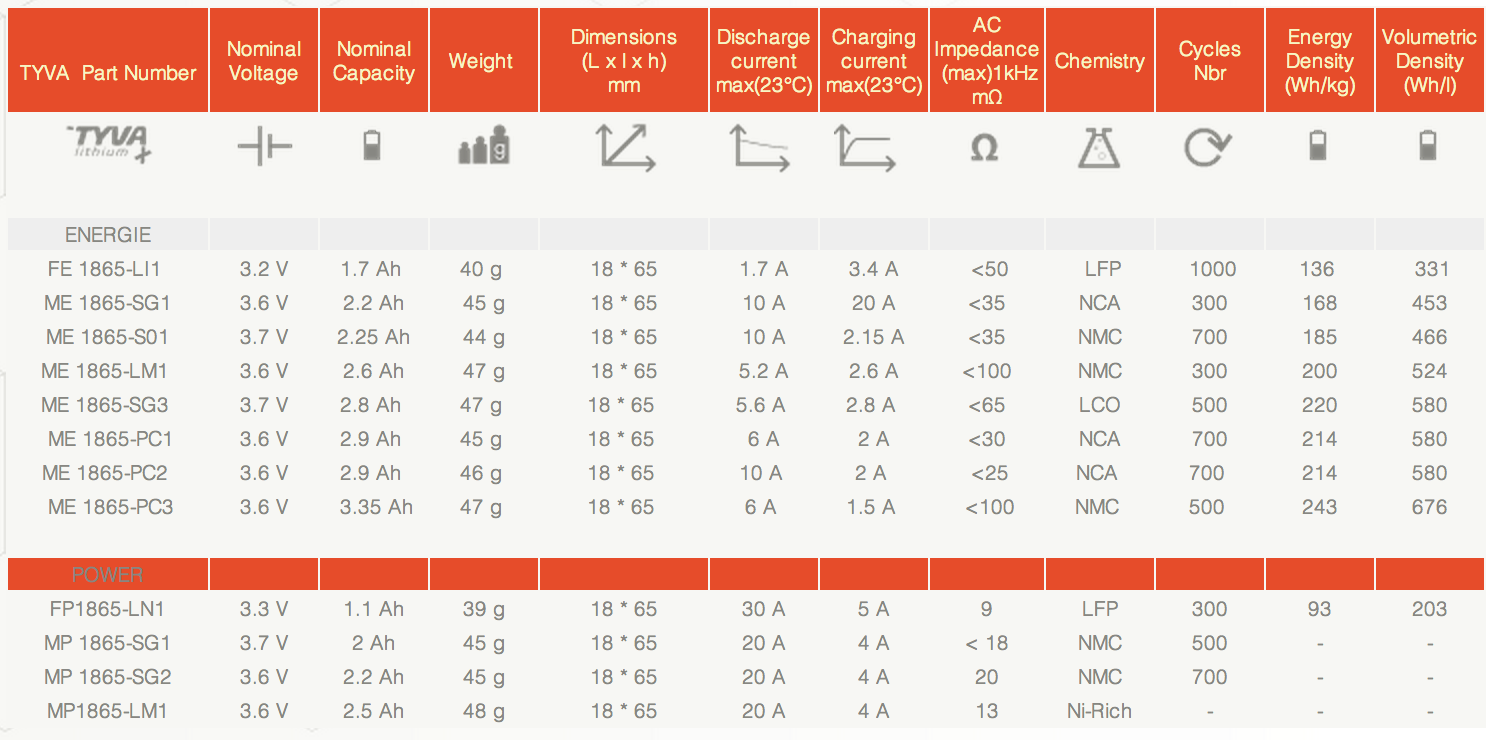
\includegraphics[height=4cm]{tyva_batteries.png}}\\
    \caption{}
    \label{fig:tyva_batteries}
\end{figure}

However, using Poppy away from any power source is still possible. Is it indeed rather simple to connect external 12V battery. Such battery can be easily found over Internet and has already been tested with Poppy for an artistic project where Poppy had to be surrounded by nature\footnote{see associated project on our forum}.






% !TEX root = ../../thesis.tex

\section{Aesthetic design of the head } % (fold)
\label{sec:head-design}
A lot of effort has been put into the design and aesthetic of Poppy's head (see \figurename~\ref{fig:poppy_head_beta}) because it is both its identity and main communication apparatus.
From an aesthetic point of view, its design was inspired of course by existing robots, but also by animals, objects and art. Insights into our  main inspirations are displayed on the board in \figurename~\ref{fig:head_inspiration}. We tried to achieve a design that is cute, expressive and above all, simple.

\begin{figure}[p]
    \begin{center}
        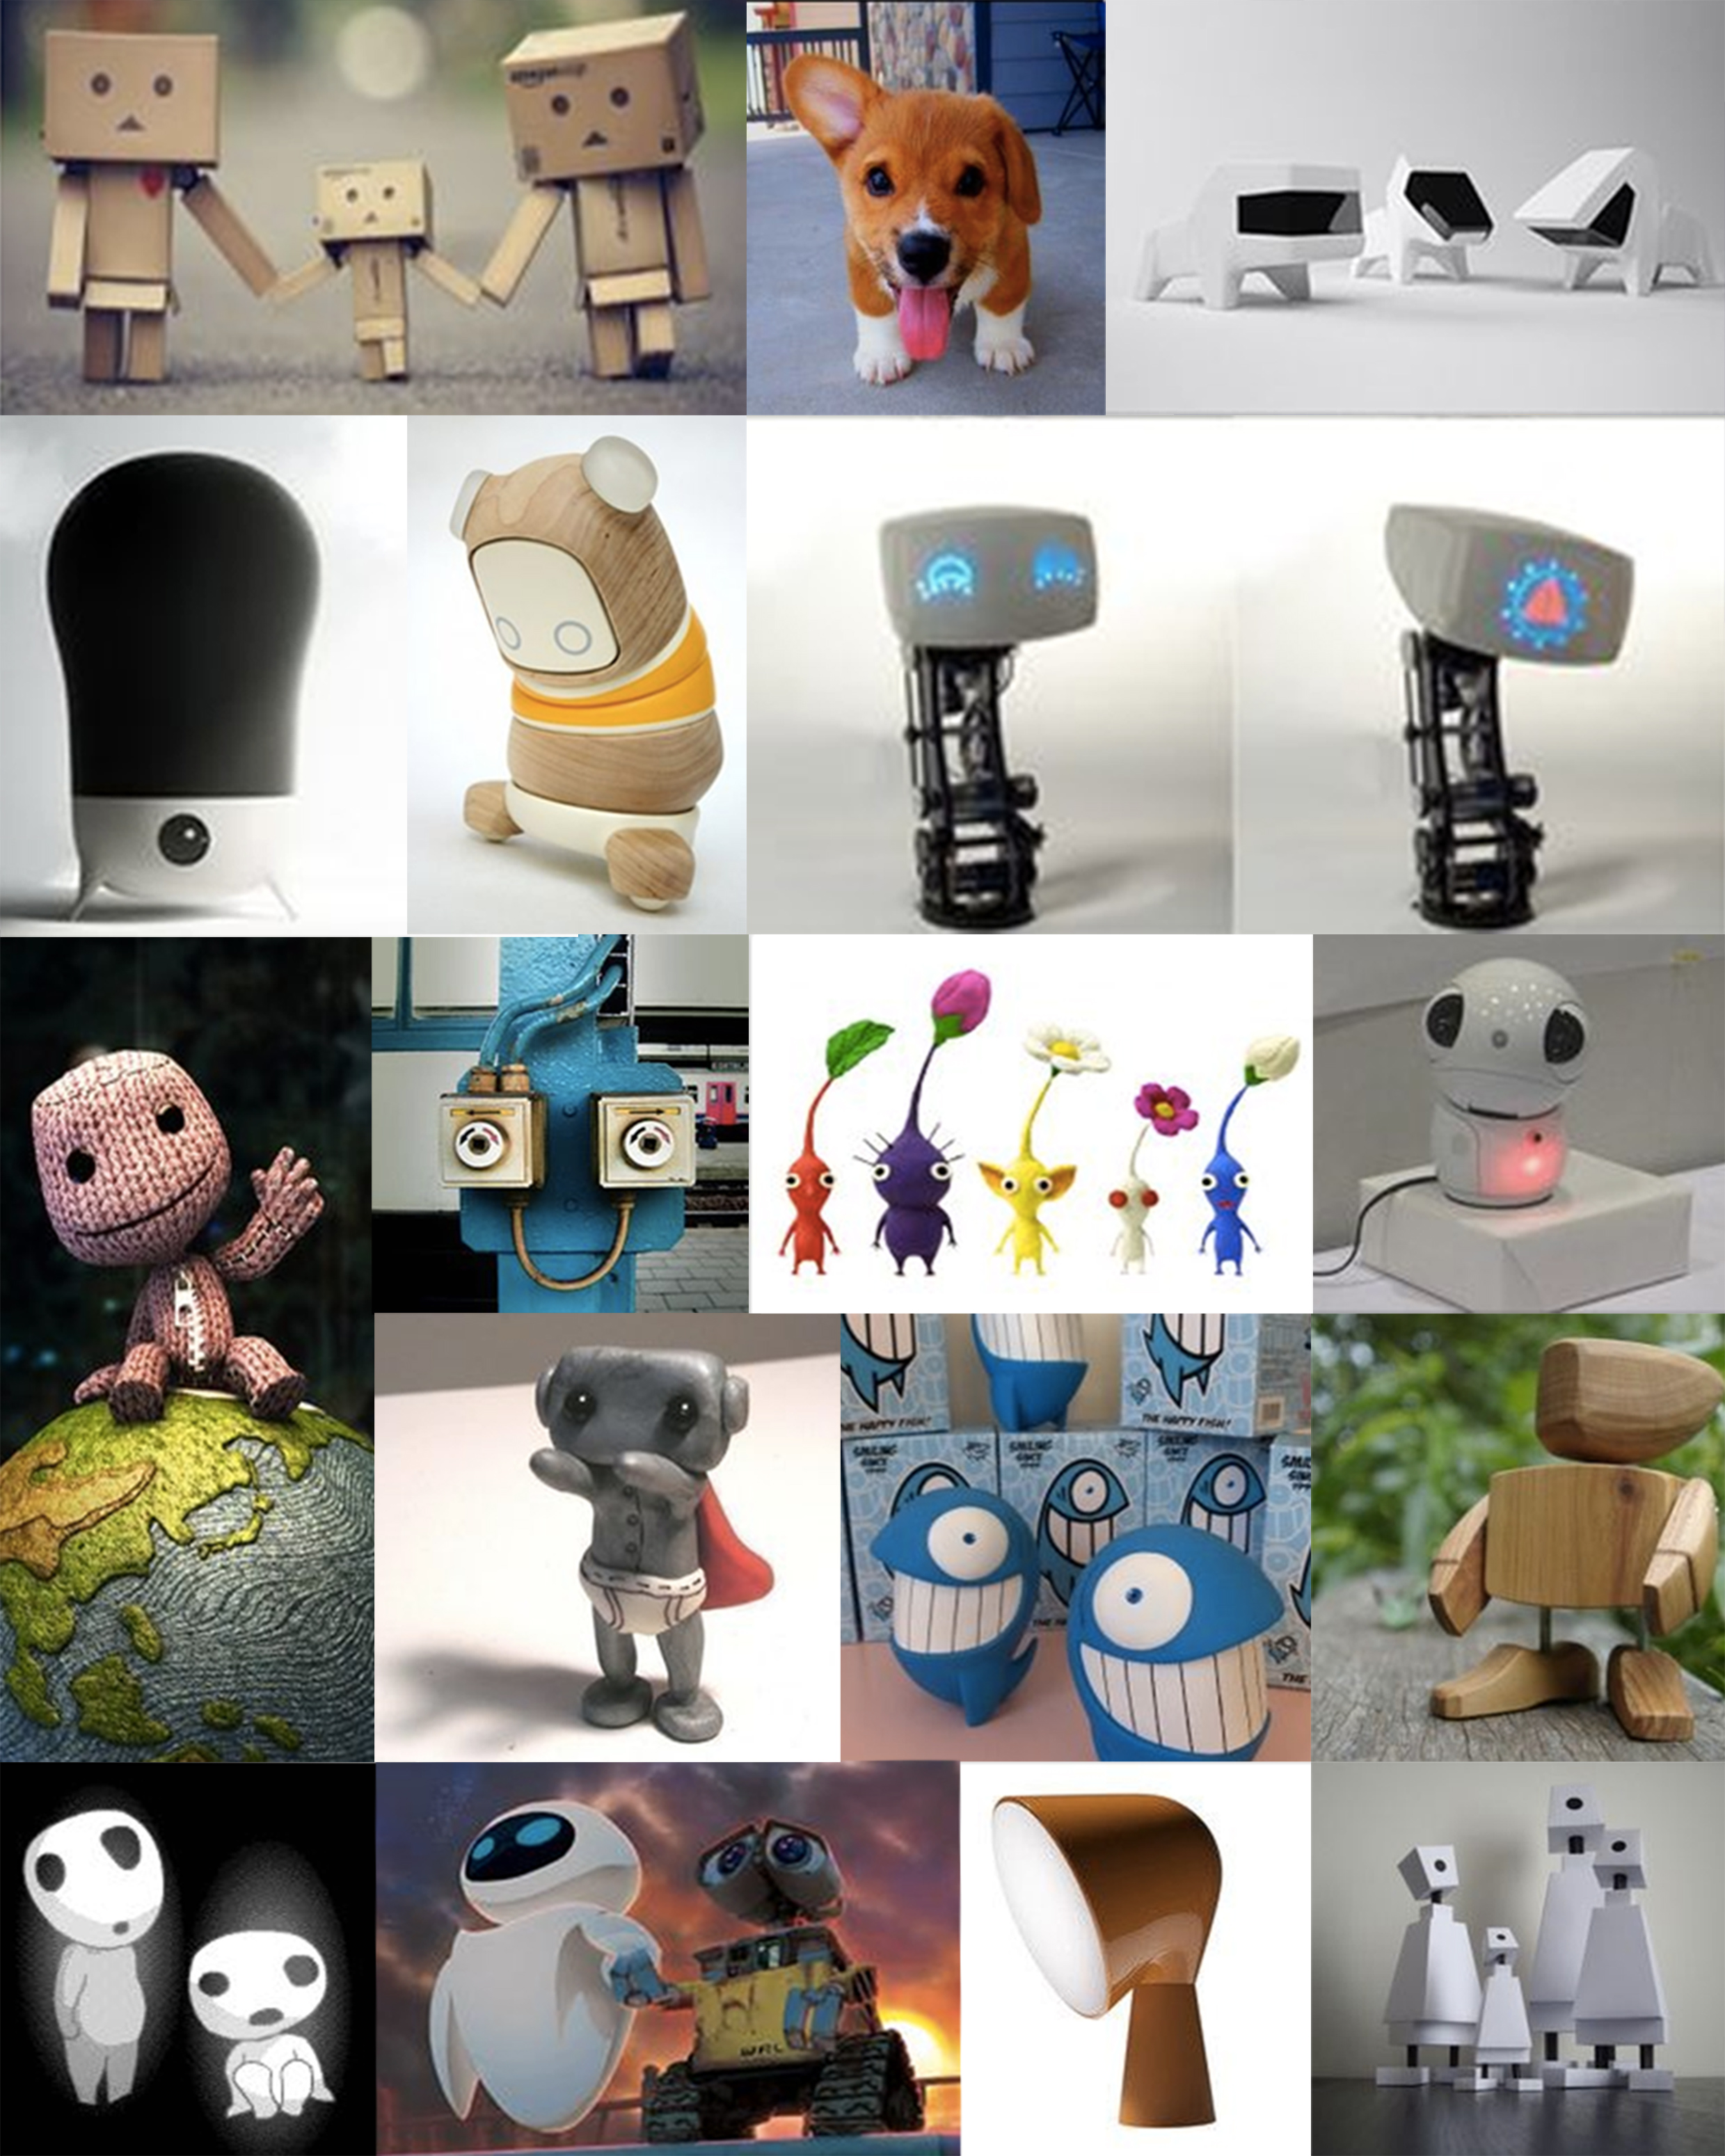
\includegraphics[width=\linewidth]{head_inspiration.jpg}
    \end{center}
    \caption{Complete board available on pinterest \url{http://www.pinterest.com/matthieulapeyre/robot/}}
    \label{fig:head_inspiration}
\end{figure}

\begin{figure}[p]
\centering
    \subfloat[][]{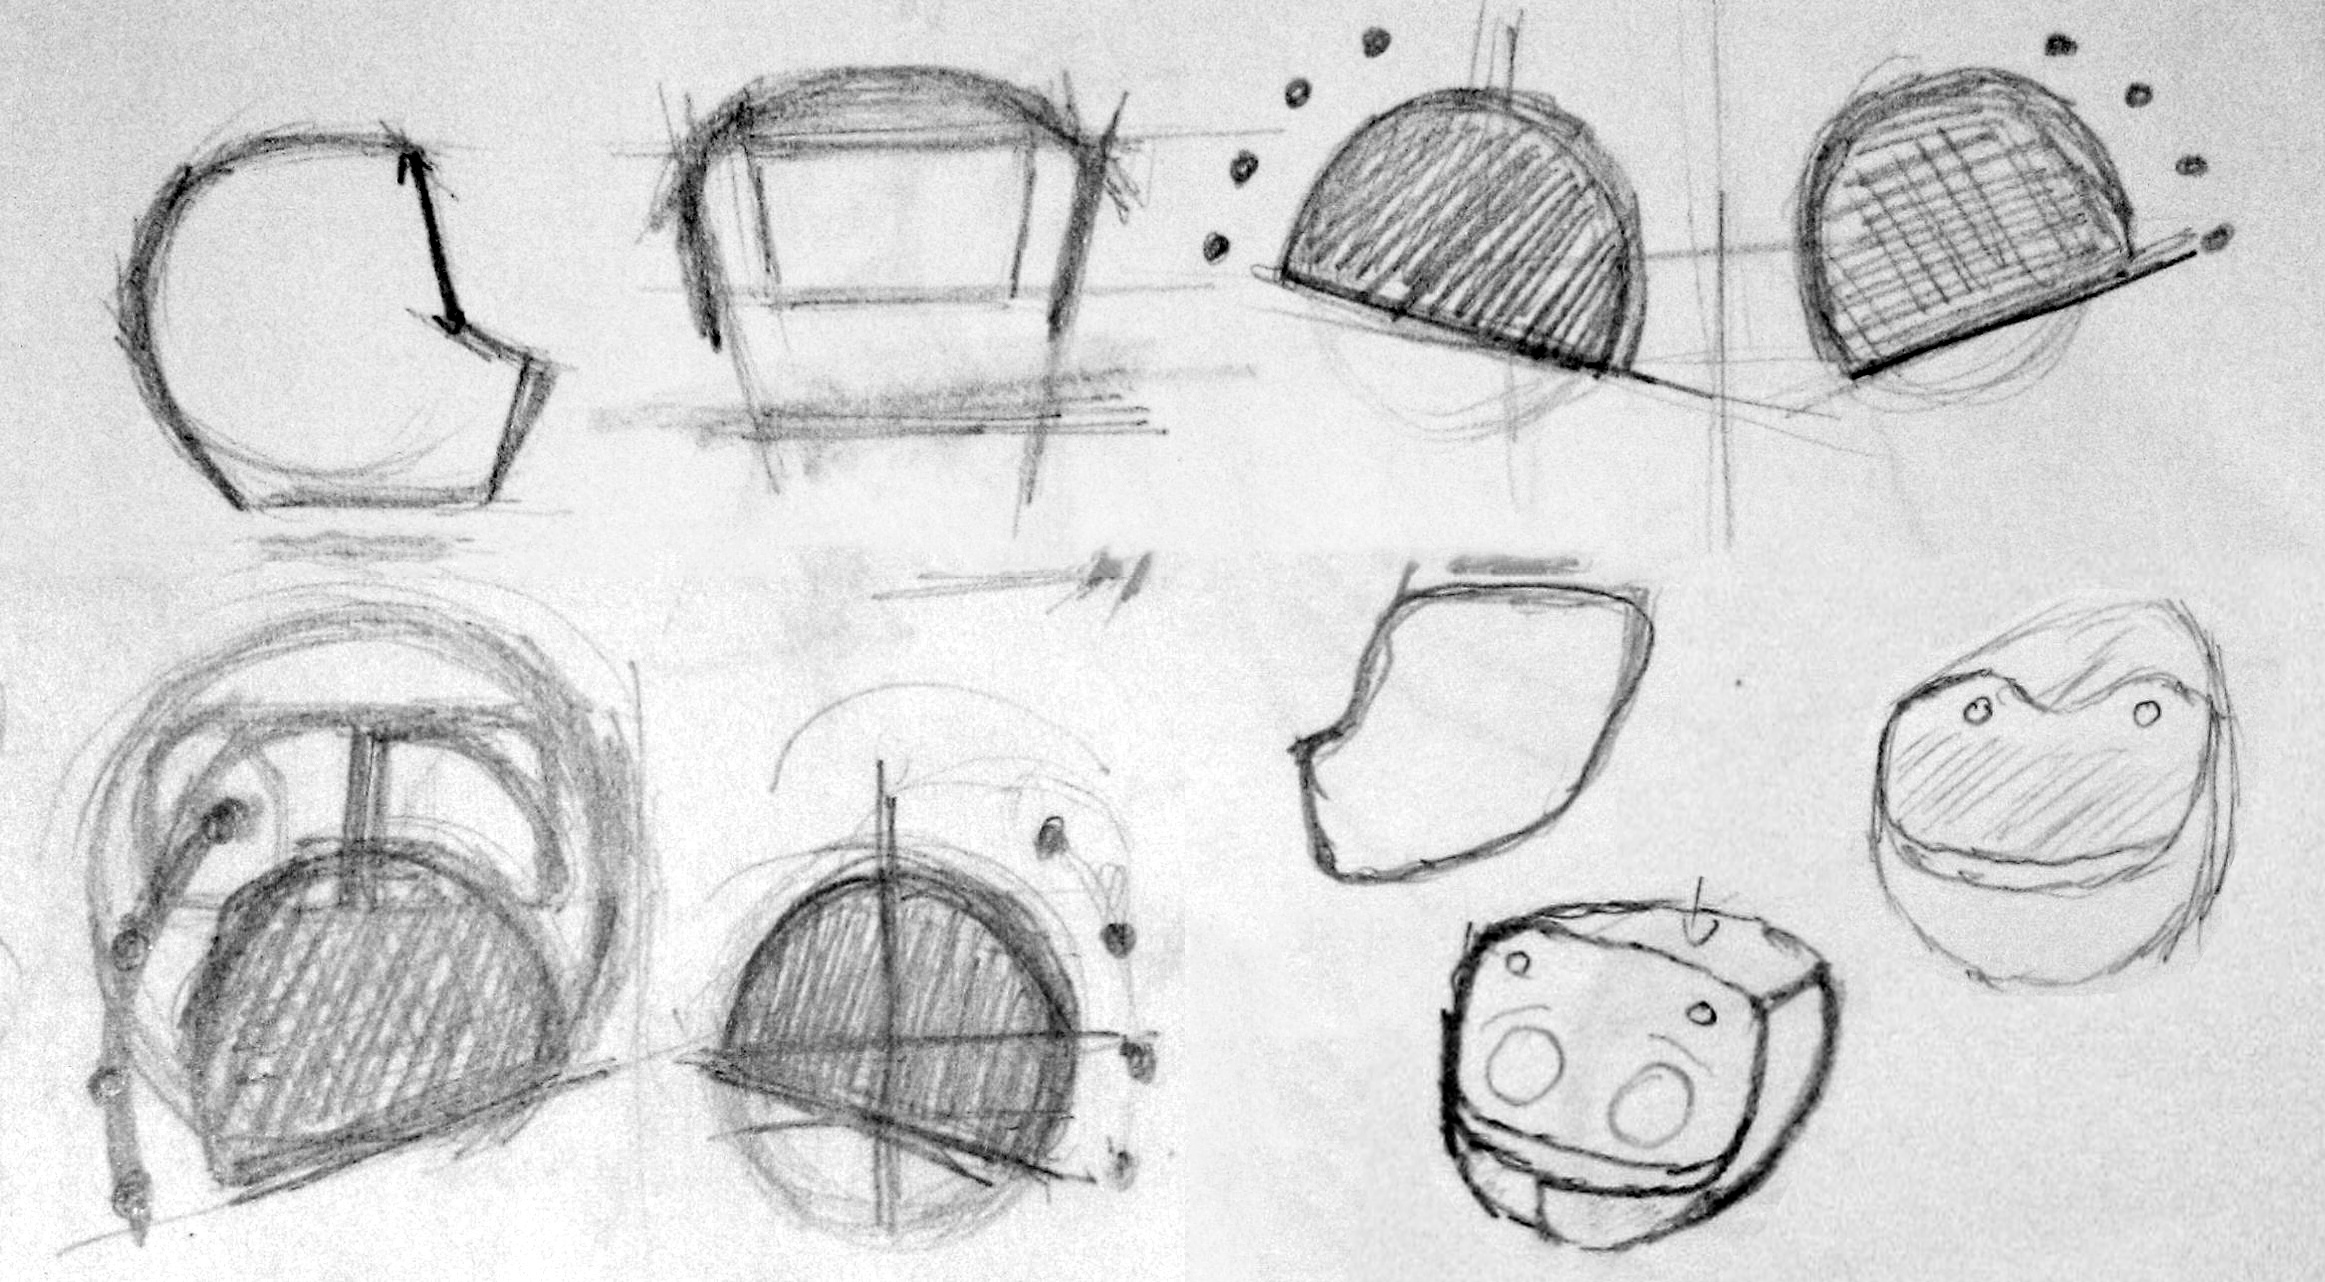
\includegraphics[height=4.5cm]{first_sketch.jpg}}
    \hfill
    \subfloat[][]{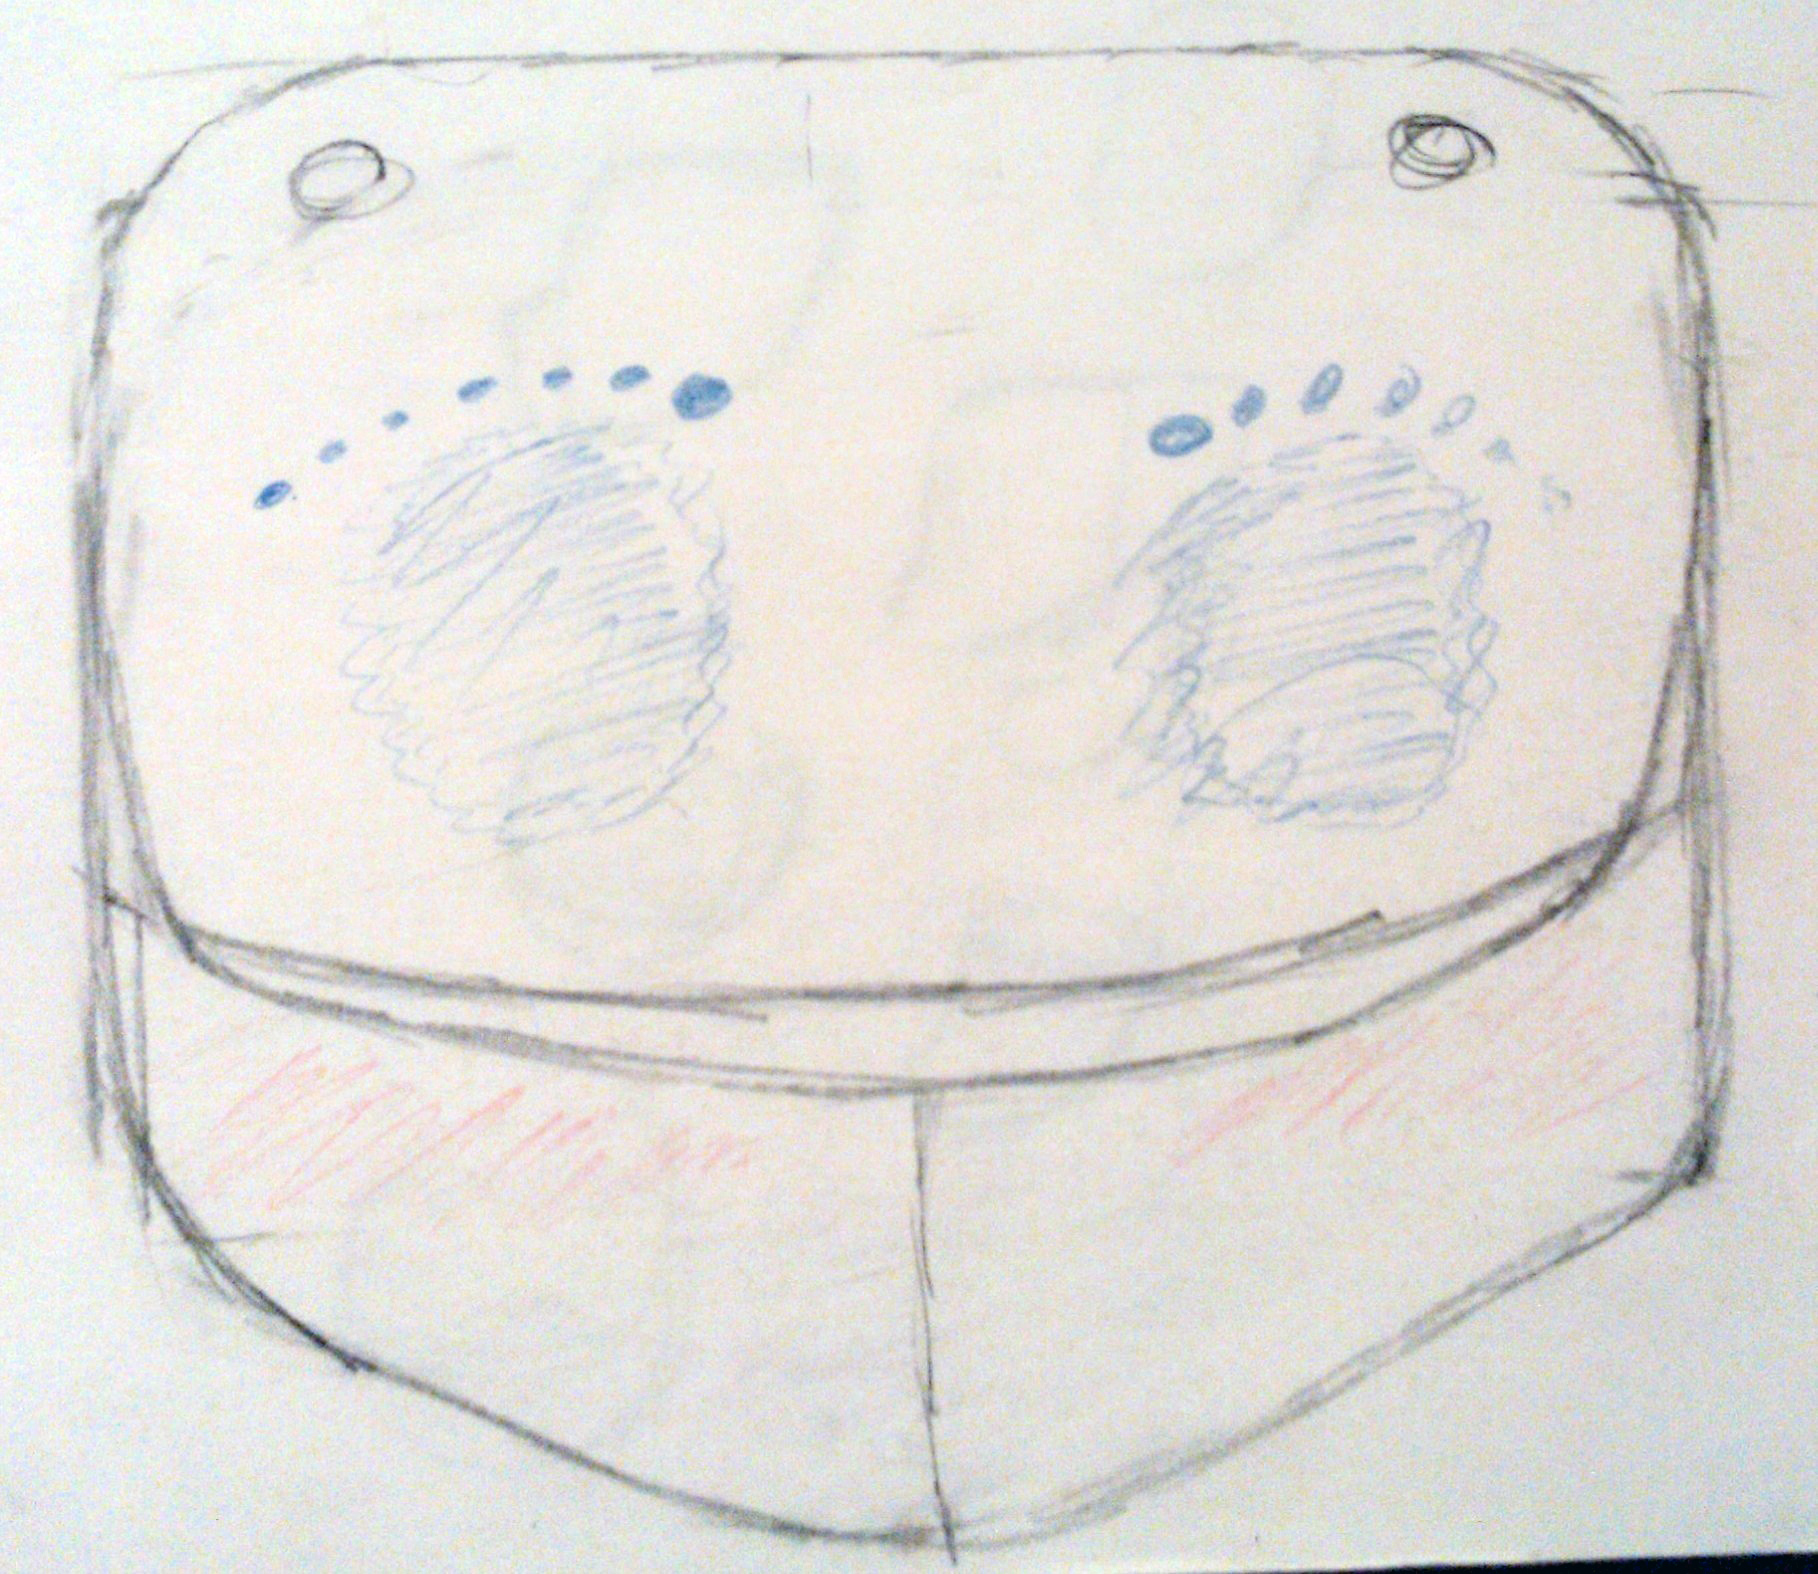
\includegraphics[height=4.5cm]{poppy_head_sketch.jpg}}\\
    \subfloat[][First clay sculpture]{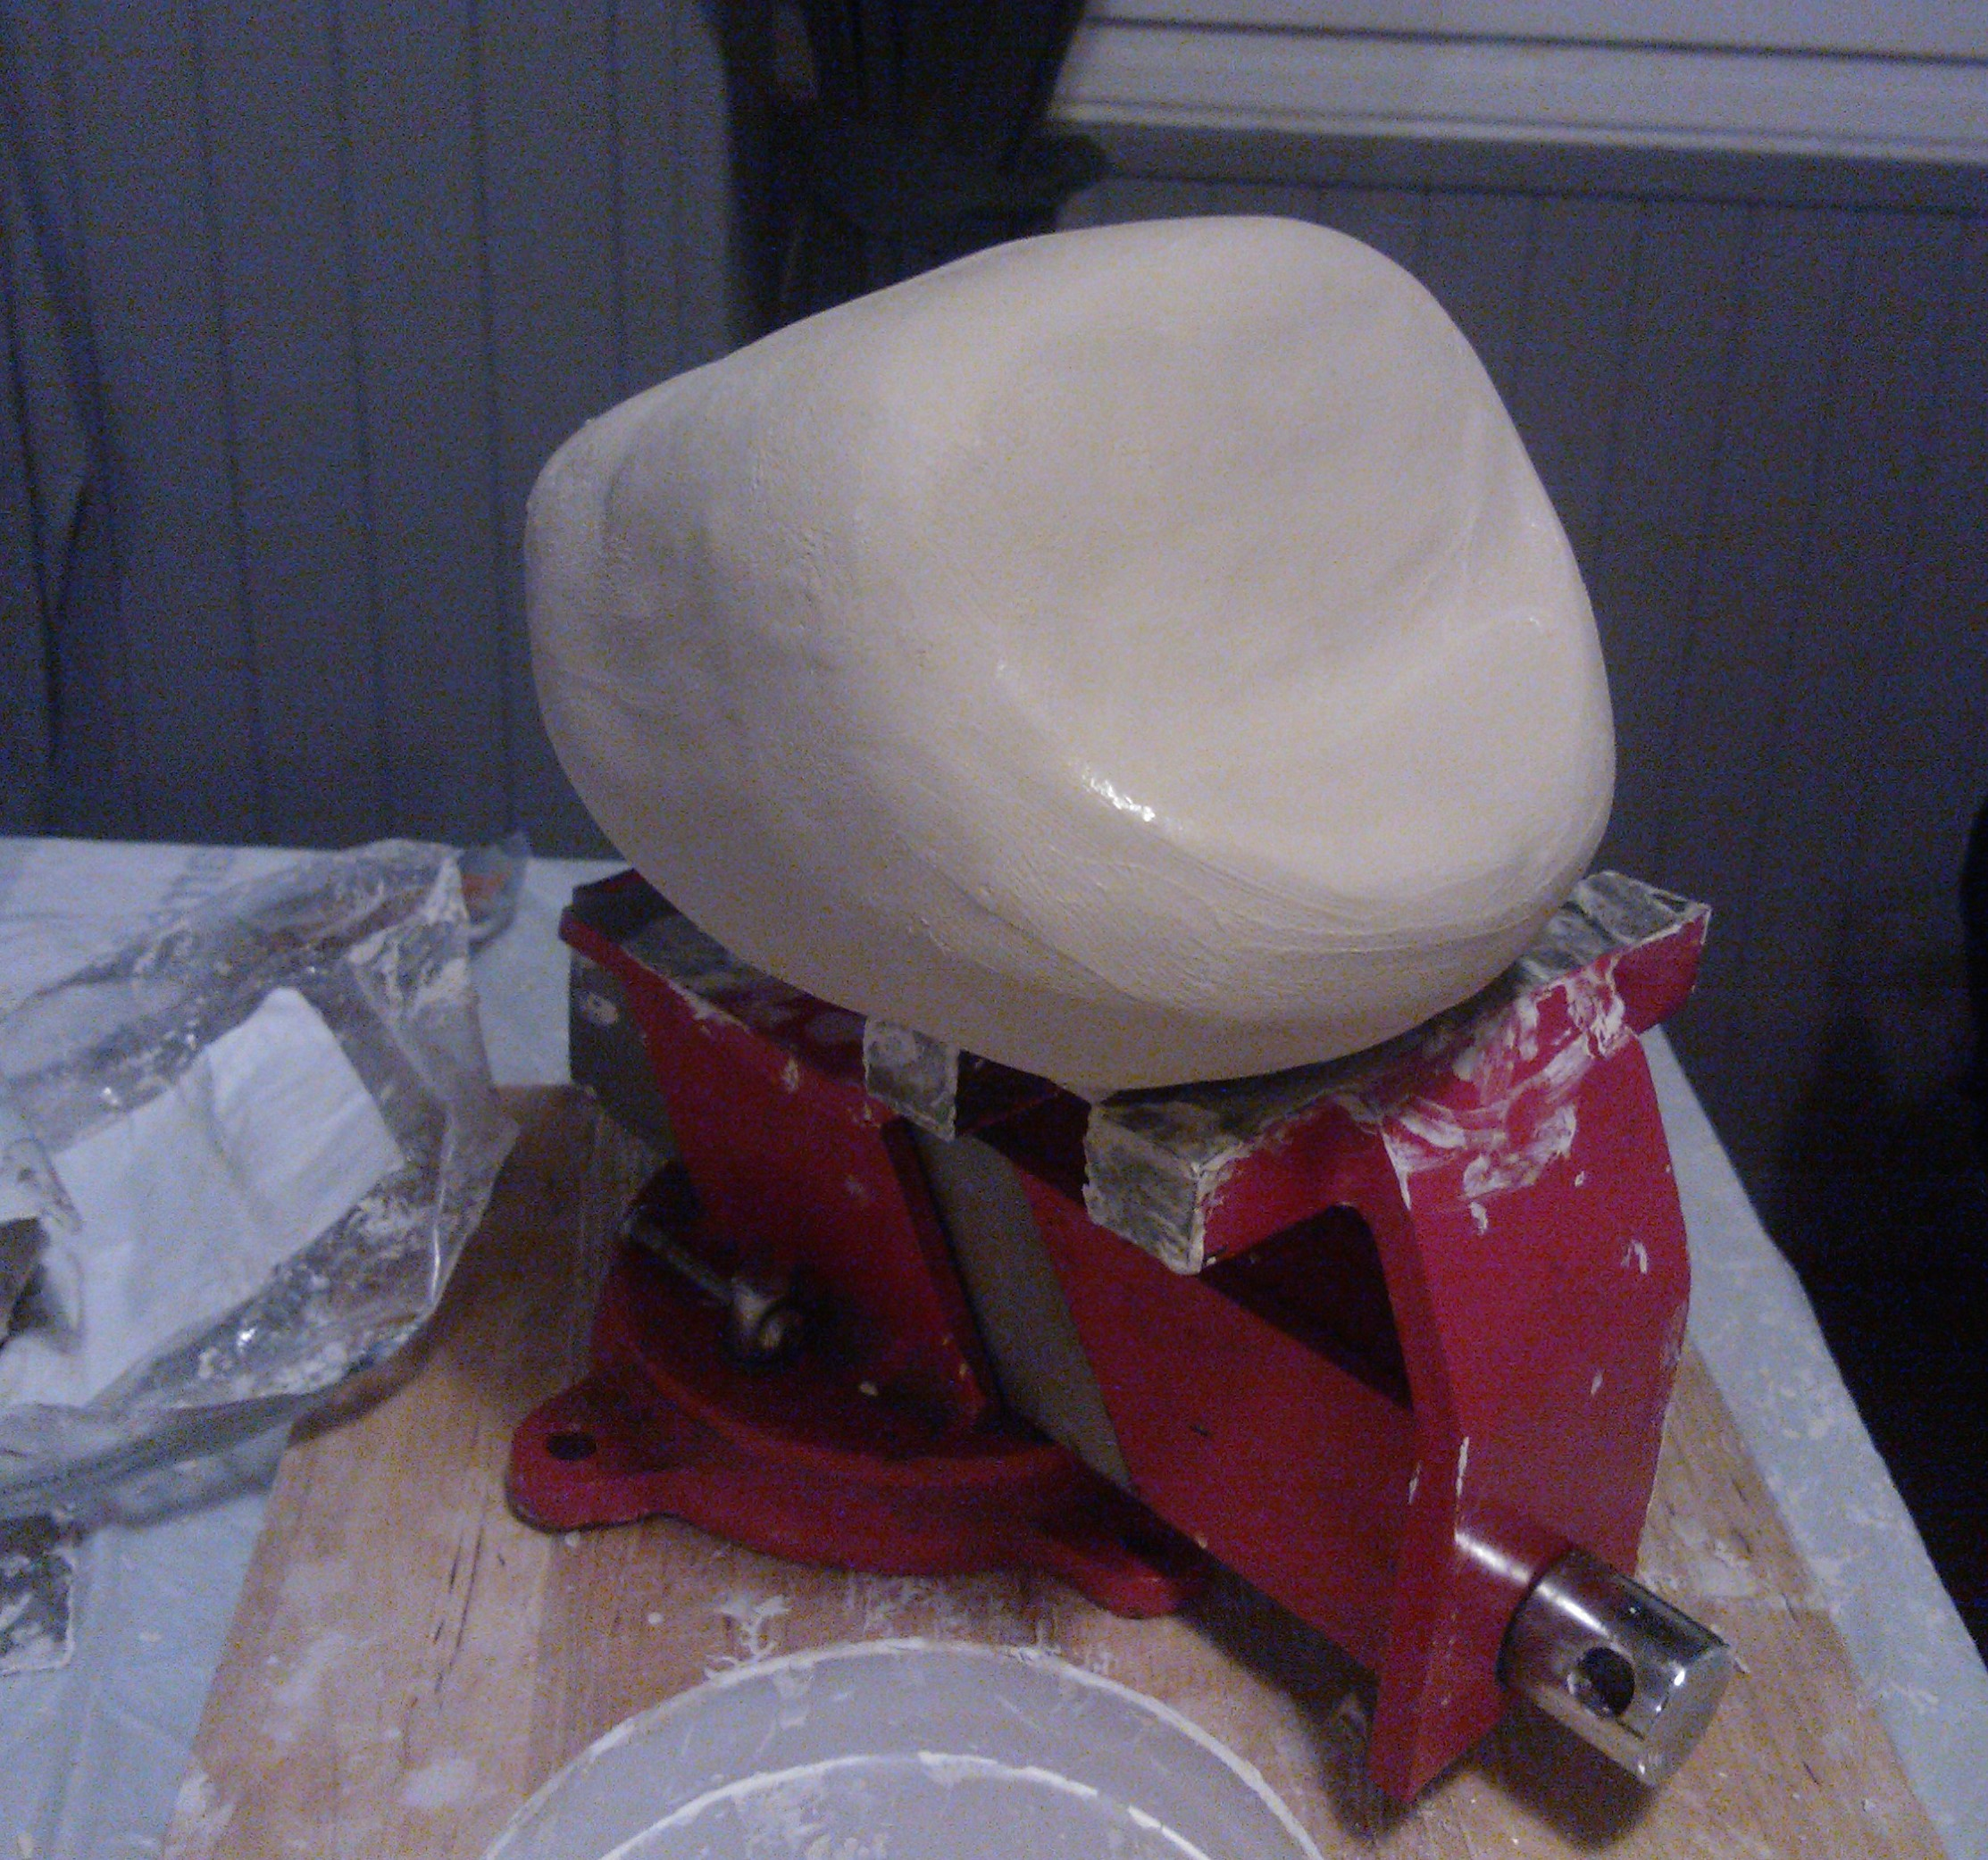
\includegraphics[height=5.5cm]{first_poppy_clay.jpg}}
    \hfill
    \subfloat[][First CAO model]{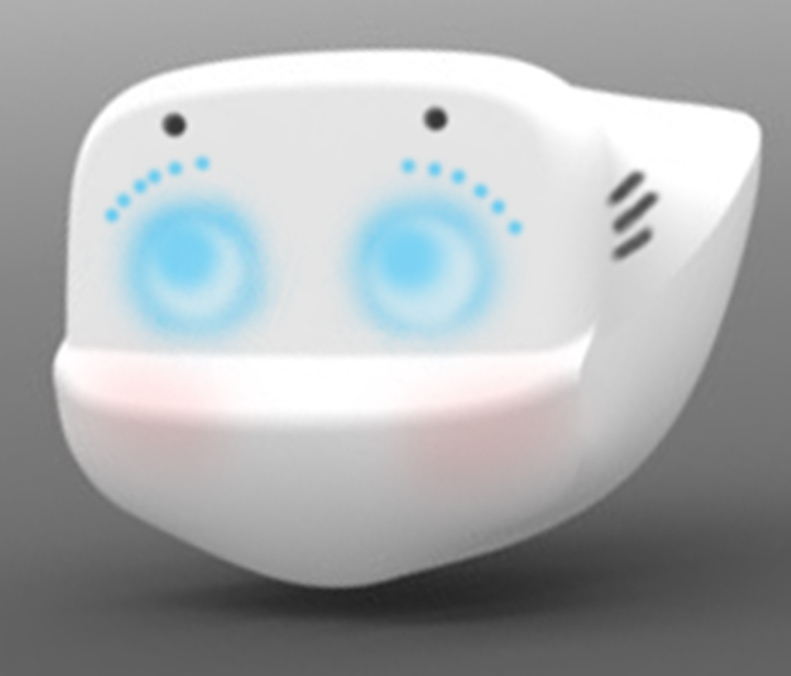
\includegraphics[height=5.5cm]{head_first_trial.jpg}}\\
    \subfloat[][Poppy beta]{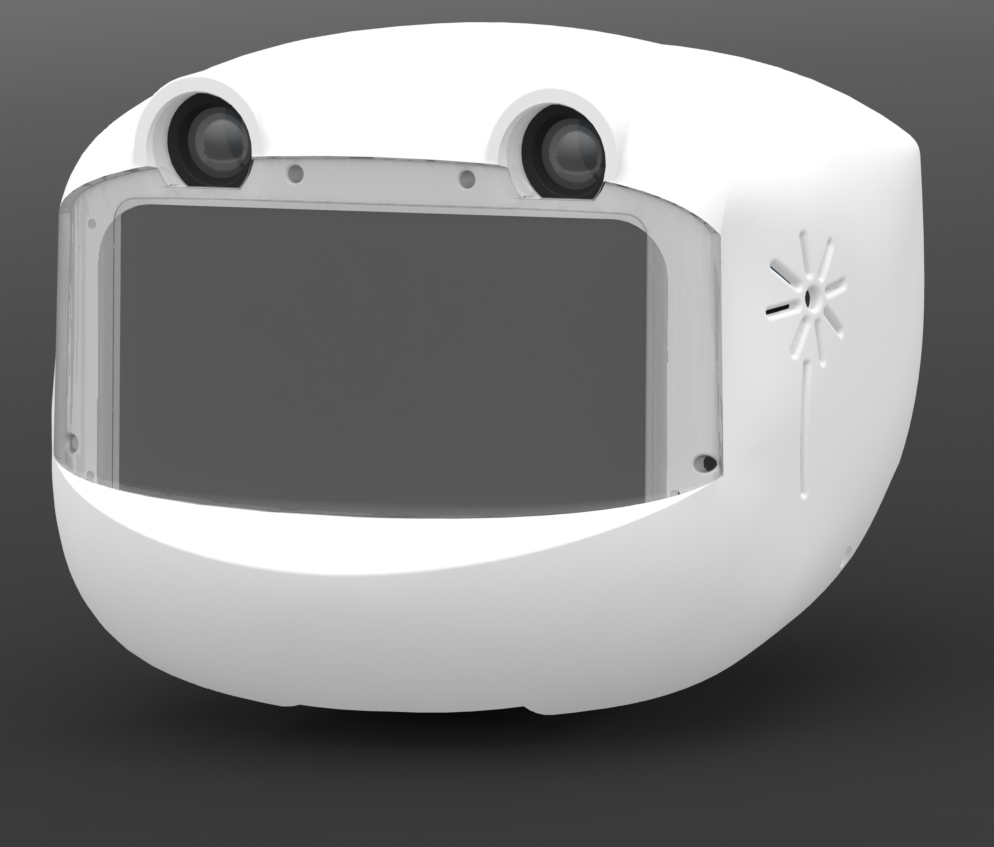
\includegraphics[height=5.5cm]{head_beta.jpg}}
    \hfill
    % \subfloat[][The first assembly]{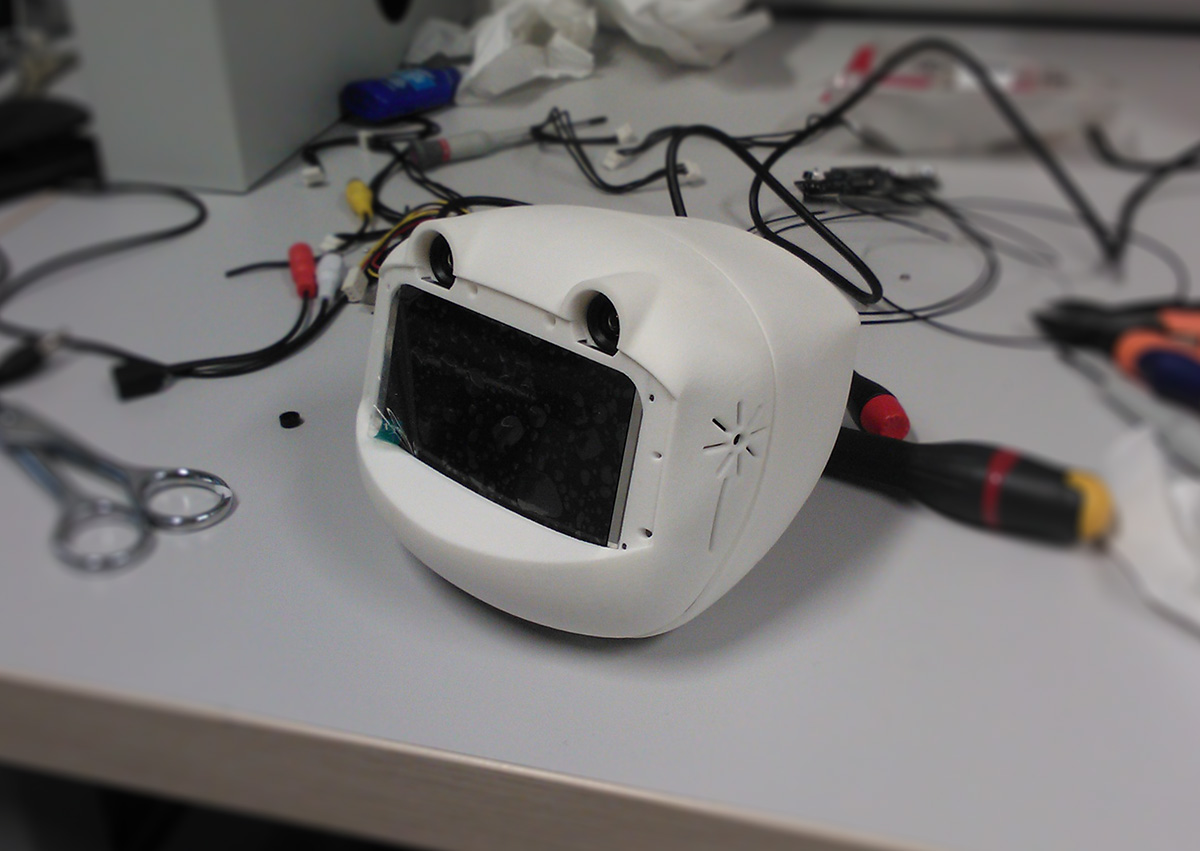
\includegraphics[height=5.5cm]{head_beta_assembled.jpg}}
    % \hfil
    \subfloat[][Screen with basic eyes display]{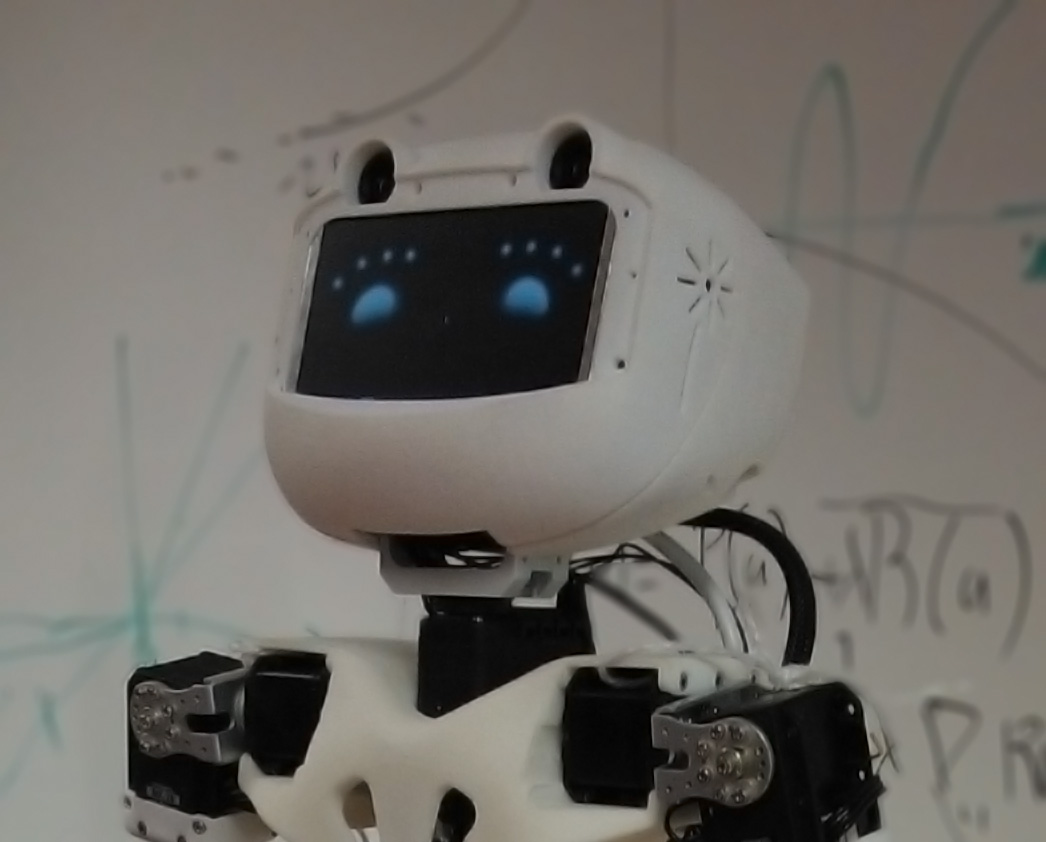
\includegraphics[height=5.5cm]{poppy_beta_eyes.jpg}}
    \caption{Evolution of Poppy’s head from the first sketches to the Poppy beta version.}
    \label{fig:poppy_head_beta}
\end{figure}

Yet because of the multi-articulated vertebral column, there is only free room in Poppy’s head to embed all electronics components needed. Therefore strong technical constraints were imposed because all electronic architecture plus the communication sensorimotor apparatus composed by a wide 4.3" screen, cameras, and audio devices all have to be embedded in the head.
These components strongly constrained the design of the robot. Especially the screen, which necessitated a large flat part on the face. Obtaining a nice, rounded head shape with such constraints was rather difficult and require several iterations before obtaining the first correct finished version (see \figurename~\ref{fig:poppy_head_beta}).

This process firstly involved several sketches showing the main ideas of the desired design. But the transfer to CAD modelling was quite complex; these kinds of shape are rather difficult to design using parametric tools. The use of clay sculpting was very helpful  in the transition from the 2D drawing to the 3D shape.




However, in the first beta version showed in \figurename~\ref{fig:poppy_head_beta}, there is a major design error. Indeed our desire was to have a screen to create and explore freely expressive eyes but the use of two visible cameras changed the way people saw Poppy's head. Of course, when people see two cameras they consider them to be the eyes of the robot and therefore extrapolate that the screen may be the mouth or another face part.

We are currently working on the new design of Poppy's head and we simply addressed this issue by replacing the two big camera by a small one with a pinhole lens, which can be hidden on Poppy’s face see \figurename~\ref{fig:poppy_head_v1}.

\begin{figure}[tb]
\centering
    % \subfloat[][Mix between Poppy beta 3D printed head and clay sculpture]{\includegraphics[height=5cm]{second_poppy_clay.jpg}}
    % \newline
    \subfloat{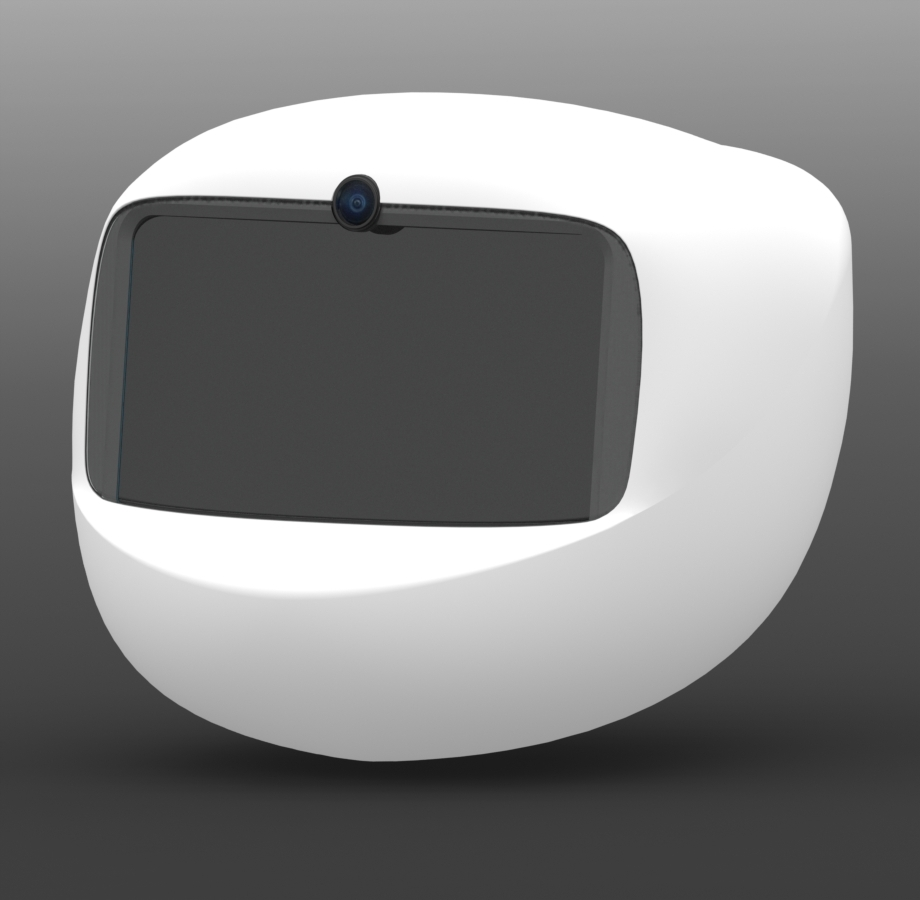
\includegraphics[width=0.6\linewidth]{poppy_v1_head.jpg}}
    \caption{A preview of the new design for Poppy's head. As we want to show expressiv eyes on the screen, we have replaced the two cameras with big lenses of Poppy beta by a small one, thus cameras are not misunderstood as Poppy's "eyes". }
    \label{fig:poppy_head_v1}
\end{figure}


While this work it is still in progress, we will update this section afterwards with a blueprint of the electronic integration and final design explanation.



\section{Limitations} % (fold)

The design and the choices we made have raised several limitations:

\subsection{Simplicity} % (fold)
Creating a robot  for which one of the main objectives is to be easy to duplicate imposes strong constraints on the design. As we saw in chapter~\ref{cha:experimental-methods}, humanoid robots often have a complex design involving many components. Achieving such complexity is not possible if we want to keep the robot easy and quick to assemble by non-expert users. Therefore, Poppy's mechanics are simple, with only one part per motor. However there are several joints whose performance could be improved by changing the design. For example, just by adding a complementary mechanism such as a reduction gear, we could increase the applied torque on critical joint (e.g. knee, ankle, hip).

\subsection{No hands} % (fold)
The current version of Poppy does not have articulated hands. The grasping ability was not a top priority and is challenging, so we preferred to only design fixed hands. There are several laboratories working on this topic so we hope one of them will be interested in contributing to the Poppy project and design articulated hands. We have already been in contact with the Bristol Robotics Lab and the Open hand project for this purpose.

\subsection{Motor modularity} % (fold)
Parametric modelling is great if we want to create variation of the same pattern with different dimensions. Thus, we can easily create configurations of all Robotis Dynamixel motors. Yet, if we are interested in using another motor brand, the configuration will not be direct and we will have to redo a part of the design process to ensure the compatibility.


\subsection{Electronic} % (fold)
\label{sub:electronic-limitations}

The electronics we developed are compatible with the exploration of morphology for sensory space because they have a lot of I/O ports to extend Poppy's sensorimotor space. Yet there are several limitations that make the final solution unsatisfactory.

Commonly used electronic components are not designed for robotic integration but rather for building small personal computers. Thus even if the electronic boards are often quite small, they have big common connectors such as USB, HDMI and Ethernet, which are of course never placed exactly where they should be for integration on the robot.
Above all, cables are really annoying; they take up a surprising amount of room (connector size, the wire length and they are heavy) while being totally useless for our applications.

Also the size of the IO Board is finally fairly big, more so than expected and while it is still compatible with Poppy’s design, it is too large, with a shape that is too strange to be appropriate for other open source projects.

Great open source projects keep their work modular so other projects can use one or several modules directly. Therefore the IO Board is not compatible with such principles and we are currently moving toward building modular Poppy electronics (we will discuss this new version in the discussion see section~\ref{sec:improve-hardware-modularity}). Yet this IO Board was the first electronic board developed in the Poppy project and through the experience we acquired a better understanding of electronic integration.



\section{Conclusion} % (fold)

Thanks to the methodology presented in the chapter~\ref{cha:methodology}, the design and production of a completely new humanoid robot has been very fast and low cost. Indeed, the project began at the end of May 2012 and the first fully-functional version of Poppy (the one we can see in \figurename~\ref{fig:TER_cognitic}) was presented at the end of September 2012 at Collège de France. The cumulative work of all the different people involved was equivalent to about 8 months and cost less than \texteuro10,000 in material.

Because of the lack of easy and cheap tooling to produce a custom electronics board, the new design of the electronic architecture took more time and several elements are still in progress for.


\begin{figure}[tb]
    \begin{center}
        \includegraphics[width=\linewidth]{poppy_components.jpg}
    \end{center}
    \caption{Time lapse of the assembly is available here: \url{https://vimeo.com/96262428}}
    \label{fig:poppy_components}
\end{figure}

Yet Poppy cost about \texteuro8,000 and it only takes one or two days to assemble (see \figurename~\ref{fig:poppy_components}). Also its morphological design allows for modularity both for the mechanics, as the parametric parts can be easily customized and reprinted, and for the electronics thanks to the compatibility with the Arduino environment. This modularity is completed by the control library which will be presented in the next chapter.

Examples of variations in Poppy’s morphology will be presented in chapter~\ref{cha:changing_morphology}. Also thanks to its simple design, Poppy can be relevant for educational and artistic purposes. Applications will be presented in chapter~\ref{cha:education} and chapter~\ref{cha:art}.






% If we had to do it today we would make the same mistakes.

% In particular, even if we tried to remove most of the necessary cables, we saw it is still complicated to integrate. We really have to develop a board that does not require any wires at all.

% Actually, I spent more time looking for the fitting cable on the web than thinking about the electronics architecture. The wire-problem is often under-estimated and therefore becomes one of the biggest problems for robotics. We experienced the same issue during the ergo-robot experiment and during the use of Poppy with artists (see chapter REF). So basically, the wire problem is one of the most overlooked issues…






